% ============================================================
%  THE FATE OF DISTINGUISHABILITY
%  Author: Flyxion
%  Engine: LuaLaTeX
%  Build:  lualatex fate-of-distinguishability &&
%          biber fate-of-distinguishability &&
%          lualatex fate-of-distinguishability &&
%          makeindex fate-of-distinguishability.idx &&
%          lualatex fate-of-distinguishability &&
%          lualatex fate-of-distinguishability
%
%  Middle volume of the trilogy:
%    I.  Persistence Before Truth
%    II. The Fate of Distinguishability   <-- this volume
%    III. The Ecology of Distinctions
% ============================================================
\documentclass[12pt,twoside,openright]{book}

% ---- Fonts -------------------------------------------------
\usepackage{fontspec}
\setmainfont{TeX Gyre Pagella}
\setsansfont{TeX Gyre Heros}
\setmonofont[Scale=0.85]{TeX Gyre Cursor}
% On your system with TeX Gyre Pagella Math installed:
% \usepackage{unicode-math} % needs Pagella Math on your system
% \setmathfont{TeX Gyre Pagella Math}
% Sandbox note: if Pagella Math is unavailable, comment the two lines above
% and add \usepackage{amsmath,amssymb} before \usepackage{amsthm,mathtools}

% ---- Geometry ----------------------------------------------
% Matches The Ecology of Distinctions exactly
\usepackage[paperwidth=17cm,paperheight=24cm,
  top=2.5cm,bottom=2.8cm,inner=2.8cm,outer=2.2cm,
  marginparwidth=1.4cm,marginparsep=0.3cm]{geometry}

% ---- Colour ------------------------------------------------
% Full palette inherited from The Ecology of Distinctions
\usepackage[dvipsnames,svgnames,x11names]{xcolor}
\definecolor{DistBlue}  {HTML}{1B4F72}
\definecolor{DistTeal}  {HTML}{117A65}
\definecolor{DistAmber} {HTML}{B7770D}
\definecolor{DistRed}   {HTML}{922B21}
\definecolor{DistGray}  {HTML}{566573}
\definecolor{DistGold}  {HTML}{7D6608}
\definecolor{DistLight} {HTML}{EAF4FB}
\definecolor{DistLightG}{HTML}{E9F7EF}
\definecolor{DistGoldBg}{HTML}{FEF9E7}
\definecolor{DistSage}  {HTML}{5B7553}
\definecolor{DistSageBg}{HTML}{F1F5EF}
% New accent for the middle volume — fate geometry uses violet
\definecolor{FateViolet}{HTML}{4A235A}
\definecolor{FateLilac} {HTML}{F5EEF8}
\definecolor{FateStrata}{HTML}{7D3C98}

% ---- TikZ --------------------------------------------------
\usepackage{tikz,pgfplots}
\pgfplotsset{compat=1.18}
\usetikzlibrary{arrows.meta,positioning,shapes.geometric,
  decorations.pathmorphing,backgrounds,fit,calc,matrix,patterns}
\tikzset{
  thmnode/.style={rectangle,rounded corners=4pt,
    draw=DistTeal,fill=DistLight,font=\sffamily\footnotesize,
    text width=4.2cm,align=center,inner sep=4pt},
  lawnode/.style={rectangle,rounded corners=4pt,
    draw=DistGold,fill=DistGoldBg,
    font=\sffamily\footnotesize\bfseries,
    text width=4.2cm,align=center,inner sep=4pt},
  fatenode/.style={rectangle,rounded corners=4pt,
    draw=FateViolet,fill=FateLilac,
    font=\sffamily\footnotesize,
    text width=4.2cm,align=center,inner sep=4pt},
  thmedge/.style={-Stealth,DistTeal,thick},
  fateedge/.style={-Stealth,FateViolet,thick},
  distnode/.style={circle,draw=DistBlue,fill=DistLight,
    minimum size=7mm,font=\small\sffamily},
  distedge/.style={-Stealth,DistTeal,thick},
}

% ---- Chapter/section style ---------------------------------
\usepackage{titlesec}
\titleformat{\chapter}[display]
  {\sffamily\bfseries\color{DistBlue}\huge}
  {\color{DistTeal}\sffamily\Large\chaptername\ \thechapter}
  {0.5ex}{\titlerule[1pt]\vspace{0.8ex}}[\vspace{0.4ex}\titlerule]
\titleformat{\section}
  {\sffamily\bfseries\large\color{DistBlue}}{\thesection}{1em}{}
\titleformat{\subsection}
  {\sffamily\bfseries\normalsize\color{DistGray}}{\thesubsection}{1em}{}

% ---- Headers/footers ---------------------------------------
\usepackage{fancyhdr}
\pagestyle{fancy}\fancyhf{}
\fancyhead[LE]{\small\sffamily\color{DistGray}\leftmark}
\fancyhead[RO]{\small\sffamily\color{DistGray}\rightmark}
\fancyfoot[C]{\small\sffamily\thepage}
\renewcommand{\headrulewidth}{0.4pt}

% ---- Maths -------------------------------------------------
\usepackage{amsmath,amssymb,amsthm,mathtools}
\usepackage[most]{tcolorbox}

% ---- Theorem environments ----------------------------------
% Matches EOD exactly: tcolorbox newtcbtheorem, numbered by chapter
% Syntax: \begin{theorem}{Display Name}{label-suffix} ... \end{theorem}
% Reference via: \cref{thm:label-suffix}

\tcbset{thmbase/.style={enhanced,breakable,
  left=4pt,right=4pt,top=6pt,bottom=4pt,
  fonttitle=\sffamily\bfseries,separator sign={.}}}

% Level 0 — Gold (axioms, laws, principles)
\newtcbtheorem[number within=chapter]{axiom}{Axiom}{
  thmbase,colback=DistGoldBg,colframe=DistGold,coltitle=white,
  borderline west={3pt}{0pt}{DistGold},
  attach boxed title to top left={yshift=-2mm,xshift=4mm},
  boxed title style={colback=DistGold,rounded corners}}{axm}
\newtcbtheorem[use counter from=axiom]{law}{Law}{
  thmbase,colback=DistGoldBg,colframe=DistGold!80,coltitle=white,
  borderline west={3pt}{0pt}{DistGold!80},
  attach boxed title to top left={yshift=-2mm,xshift=4mm},
  boxed title style={colback=DistGold!80,rounded corners}}{law}
\newtcbtheorem[use counter from=axiom]{principle}{Principle}{
  thmbase,colback=DistGoldBg,colframe=DistGold!60,coltitle=white,
  borderline west={3pt}{0pt}{DistGold!60},
  attach boxed title to top left={yshift=-2mm,xshift=4mm},
  boxed title style={colback=DistGold!60,rounded corners}}{prc}

% Level 1 — Teal (theorems)
\newtcbtheorem[number within=chapter]{theorem}{Theorem}{
  thmbase,colback=DistLight,colframe=DistTeal,coltitle=white,
  attach boxed title to top left={yshift=-2mm,xshift=4mm},
  boxed title style={colback=DistTeal,rounded corners}}{thm}

% Level 1 variant — Violet (meta-level theorems about the operator algebra)
% Reserved for theorems whose subject is the fate framework itself,
% not its applications. E.g., Meta-Stability Theorem, Collapse Discontinuity.
\newtcbtheorem[use counter from=theorem]{metatheorem}{Meta-Theorem}{
  thmbase,colback=FateLilac,colframe=FateViolet,coltitle=white,
  attach boxed title to top left={yshift=-2mm,xshift=4mm},
  boxed title style={colback=FateViolet,rounded corners}}{meta}

% Level 2 — Blue (propositions)
\newtcbtheorem[use counter from=theorem]{proposition}{Proposition}{
  thmbase,colback=DistLight,colframe=DistBlue,coltitle=white,
  attach boxed title to top left={yshift=-2mm,xshift=4mm},
  boxed title style={colback=DistBlue,rounded corners}}{prop}

% Level 3 — Gray (lemmas, corollaries)
\newtcbtheorem[use counter from=theorem]{lemma}{Lemma}{
  thmbase,colback=DistLight,colframe=DistGray,coltitle=white,
  attach boxed title to top left={yshift=-2mm,xshift=4mm},
  boxed title style={colback=DistGray,rounded corners}}{lem}
\newtcbtheorem[use counter from=theorem]{corollary}{Corollary}{
  thmbase,colback=DistLight,colframe=DistTeal!50,coltitle=DistBlue,
  attach boxed title to top left={yshift=-2mm,xshift=4mm},
  boxed title style={colback=DistTeal!50,rounded corners}}{cor}

% Conjectures — Amber/gold border, open question
% Used in Chapter 17 (Phase Transitions) and wherever
% the theory identifies an unresolved question with
% enough structure to be statable precisely.
\newtcbtheorem[use counter from=theorem]{conjecture}{Conjecture}{
  thmbase,colback=DistGoldBg,colframe=DistAmber,coltitle=white,
  borderline west={3pt}{0pt}{DistAmber},
  attach boxed title to top left={yshift=-2mm,xshift=4mm},
  boxed title style={colback=DistAmber,rounded corners}}{conj}

% Definitions / Examples / Remarks
\newtcbtheorem[number within=chapter]{definition}{Definition}{
  thmbase,colback=DistLightG,colframe=DistTeal,coltitle=white,
  attach boxed title to top left={yshift=-2mm,xshift=4mm},
  boxed title style={colback=DistTeal,rounded corners}}{defn}
\newtcbtheorem[number within=chapter]{example}{Example}{
  thmbase,colback=orange!5,colframe=DistAmber!80,coltitle=white,
  attach boxed title to top left={yshift=-2mm,xshift=4mm},
  boxed title style={colback=DistAmber!80,rounded corners}}{ex}
\newtcbtheorem[number within=chapter]{remark}{Remark}{
  thmbase,colback=yellow!6,colframe=DistAmber,coltitle=white,
  attach boxed title to top left={yshift=-2mm,xshift=4mm},
  boxed title style={colback=DistAmber,rounded corners}}{rmk}

% Convenience wrappers (anonymous, no label)
\newenvironment{defn}{\begin{definition}{}{}}{\end{definition}}
\newenvironment{thm}{\begin{theorem}{}{}}{\end{theorem}}
\newenvironment{lem}{\begin{lemma}{}{}}{\end{lemma}}
\newenvironment{cor}{\begin{corollary}{}{}}{\end{corollary}}
\newenvironment{prop}{\begin{proposition}{}{}}{\end{proposition}}
\newenvironment{ex}{\begin{example}{}{}}{\end{example}}
\newenvironment{rem}{\begin{remark}{}{}}{\end{remark}}

\renewcommand{\qedsymbol}{\textcolor{DistTeal}{$\blacksquare$}}

% ---- Tables / figures --------------------------------------
\usepackage{graphicx,booktabs,longtable,array,caption,subcaption}
\captionsetup{font=small,labelfont={sf,bf,color=DistBlue}}

% ---- Margin icons ------------------------------------------
\usepackage{fontawesome5,enumitem}
\newcommand{\csicon} {\marginpar{\tiny\color{DistBlue}\faCode}}
\newcommand{\bioicon}{\marginpar{\tiny\color{DistTeal}\faDna}}
\newcommand{\physicon}{\marginpar{\tiny\color{DistGray}\faAtom}}
\newcommand{\fateicon}{\marginpar{\tiny\color{FateViolet}\faSitemap}}

% ---- Index -------------------------------------------------
\usepackage{makeidx}
\makeindex

% ---- Hyperlinks --------------------------------------------
\usepackage[colorlinks=true,linkcolor=DistBlue,
  citecolor=DistTeal,urlcolor=DistAmber,
  pdftitle={The Fate of Distinguishability},
  pdfauthor={Flyxion}]{hyperref}
\usepackage{cleveref}
\crefname{tcb@cnt@theorem}{theorem}{theorems}
\Crefname{tcb@cnt@theorem}{Theorem}{Theorems}
\crefname{tcb@cnt@axiom}{axiom}{axioms}
\Crefname{tcb@cnt@axiom}{Axiom}{Axioms}
\crefname{tcb@cnt@definition}{definition}{definitions}
\Crefname{tcb@cnt@definition}{Definition}{Definitions}
\crefname{tcb@cnt@example}{example}{examples}
\Crefname{tcb@cnt@example}{Example}{Examples}
\crefname{tcb@cnt@remark}{remark}{remarks}
\Crefname{tcb@cnt@remark}{Remark}{Remarks}

% ---- Bibliography ------------------------------------------
% \usepackage[backend=biber,style=authoryear,
%   sorting=nyt,maxbibnames=6]{biblatex}
% Uncomment above and add fate.bib for bibliography support
% \addbibresource{fate.bib}

% ---- Spacing -----------------------------------------------
\usepackage{setspace}
\onehalfspacing
\usepackage{microtype}

% ============================================================
%  CUSTOM COMMANDS
% ============================================================

% --- Inherited from The Ecology of Distinctions (verbatim) ---
% Use these when cross-referencing EOD concepts.
% Do NOT redefine them here; the names are canonical.
\newcommand{\vfield}{\vec{v}}
\newcommand{\partition}{\mathcal{P}}
\newcommand{\hist}{\mathcal{H}}
% \newcommand{\reach}{\mathcal{R}} % superseded - see updated definition below
\newcommand{\adm}{\mathcal{A}}            % admissibility manifold
\newcommand{\repair}{\mathfrak{R}}        % repair operator
\newcommand{\reco}{\mathfrak{rec}}        % recoverability function rec(d)
\newcommand{\Vol}{\operatorname{Vol}}     % Vol(A(t))

% --- Inherited from Persistence Before Truth ---
% PBT uses \T, \D, \R, \X as shorthands. Here we give them
% longer descriptive names to avoid collisions.
\newcommand{\transfam}{\mathcal{T}}       % transformation family T
\newcommand{\distset}{\mathcal{D}}        % distinction set D
% IMPORTANT: PBT's \R serves double duty (reconstruction + reachability).
% This volume separates the two semantic roles clearly:
\newcommand{\recon}{\mathcal{R}_{\mathrm{rec}}}   % reconstruction operators
\newcommand{\reach}{\mathcal{R}_{\mathrm{reach}}} % reachability set/operators
% Use \recon when the operator restores a distinction after degradation.
% Use \reach when referring to the geometric reachability set from EOD.
% The shorthand \adm (inherited from EOD) covers the admissibility manifold.

% --- New: core objects of this volume ---

% The primary object: the raw distinction pair space.
% Parts I--III work directly over X x X.
% Do NOT introduce the fate-equivalence quotient here.
% The conceptual progression is:
%   X x X  -->  F  -->  (X x X)/~_F  =  \fateClasses
% The quotient appears only in Chapter 15 (Part IV, Fate Ecology).
\newcommand{\distPairs}{X\times X}

% The fate-equivalence quotient (introduced in Chapter 15 only)
% \fateClasses = (X x X) / ~_F
\newcommand{\fateClasses}{\Delta_{\mathfrak{F}}}

% The observation family
\newcommand{\obs}{\mathcal{O}}

% The fate map F: Delta_O -> S
\newcommand{\fateMap}{\mathfrak{F}}

% Fate space S = [0,1]_rho x [0,1]_eta x {0,1}_c x R^k_geq0
\newcommand{\fateSpace}{\mathcal{S}}

% Components of fate space (for inline use)
\newcommand{\survRatio}{\rho}             % survival ratio rho in [0,1]
\newcommand{\repEff}{\eta}               % repair efficiency eta in [0,1]
\newcommand{\collapseInd}{c}             % collapse indicator c in {0,1}

% The operator monoid on distinguishability
\newcommand{\distOp}{\mathsf{DistOp}}

% Fate equivalence class of a distinction pair
% Usage: \fateClass{(x,y)} gives [(x,y)]_F
\newcommand{\fateClass}[1]{[#1]_{\mathfrak{F}}}

% Fate population (measure of distinction pairs with fate class i)
% Usage: N_i(t) --- just use N_i(t) in math mode; this is for display
\newcommand{\fatePop}[1]{N_{#1}(t)}

% Distinguishability pseudometric
% d_O(x,y) = sup_{o in O} d_Y(o(x), o(y))
\newcommand{\distMetric}{d_{\mathcal{O}}}

% Survival set and ratio
\newcommand{\survSet}[1]{S_{\mathcal{T}}(#1)}    % S_T(x,y)
\newcommand{\survRat}[1]{\rho_{\mathcal{T}}(#1)} % rho_T(x,y)

% Admissible fate region (subset of S)
\newcommand{\admFate}{\mathcal{A}_{\mathfrak{F}}}

% The fate boundary (locus of discontinuities)
\newcommand{\fateBdy}{\partial\mathcal{A}}

% Persistence duration (from PBT, used in Part V)
\newcommand{\persDur}[1]{\tau(#1)}

% --- Cross-reference shorthands to outer volumes ---
% Use these in prose: "as shown in \PBT{Theorem 3.2}"
% They produce italic text with a volume tag.
\newcommand{\PBT}[1]{\textit{#1} [\textsc{pbt}]}
\newcommand{\EOD}[1]{\textit{#1} [\textsc{eod}]}

% --- Commands for Chapters 11--14 (Fate Geometry) ---

% Fate distance on a connected component of fate space
\newcommand{\fateDist}[2]{d_{\fateSpace}(#1,#2)}

% Distinction-pair distance
\newcommand{\distDist}[2]{d_{\mathcal{O}}(#1,#2)}

% Fate sensitivity at a distinction pair
\newcommand{\fateSens}[1]{\sigma_{\fateMap}(#1)}

% The singular set (locus of fate discontinuities)
\newcommand{\singSet}{\partial_{\!\mathcal{A}}}

% The four singular strata
\newcommand{\strataC}{\Sigma_{C}}   % collapse
\newcommand{\strataR}{\Sigma_{R}}   % repair threshold
\newcommand{\strataT}{\Sigma_{T}}   % transport horizon
\newcommand{\strataF}{\Sigma_{F}}   % forgetting

% Fate margin of a region U
\newcommand{\fateMargin}[1]{m(#1)}

% Admissible fate region A \subseteq S
\newcommand{\admRegion}{A}

% Admissibility operator (restriction to admissible pairs)
\newcommand{\admOp}{\pi_{\!\admRegion}}

% Object boundary
\newcommand{\objBdy}{\partial O}

% Fate-uniform predicate
\newcommand{\fateUnif}{\text{fate-uniform}}

% Lipschitz constant of the fate map
\newcommand{\fateLip}{L_{\fateMap}}

% Connected component of fate space at collapse value c
\newcommand{\fateComp}[1]{\fateSpace_{\collapseInd=#1}}

% --- Commands for Chapter 23 (Fate Theorem) and Part VI ---

% The two categories used in the Civilization theorem
% \catDist: objects = distinction pairs, morphisms = admissible operators
\newcommand{\catDist}{\mathbf{Dist}}
% \catFate: objects = fate classes, morphisms = admissible fate transformations
\newcommand{\catFate}{\mathbf{Fate}}

% The civilization functor C: Dist -> Fate
\newcommand{\civFunc}{\mathcal{C}}

% ============================================================
%  STRUCTURAL ENVIRONMENTS
% ============================================================

\newenvironment{epigraph}[2]{%
  \vspace{1em}\begin{flushright}
  \begin{minipage}{0.72\textwidth}
  \itshape\small #1\\[0.4em]
  \upshape\footnotesize\sffamily\color{DistGray}--- #2
  \end{minipage}\end{flushright}\vspace{1.5em}}{}

% Chapter objectives box (inherited from EOD)
\newenvironment{objectives}{%
  \begin{tcolorbox}[colback=DistBlue!5,colframe=DistBlue,
    title={\faCheckCircle\enspace Chapter Objectives},
    fonttitle=\sffamily\bfseries\color{white},
    attach boxed title to top left={yshift=-2mm,xshift=4mm},
    boxed title style={colback=DistBlue},breakable]
  \begin{itemize}[leftmargin=*,nosep]}{%
  \end{itemize}\end{tcolorbox}\vspace{1em}}

% Chapter summary box
\newenvironment{chapsummary}{%
  \begin{tcolorbox}[colback=DistBlue!5,colframe=DistBlue,
    title={\faBookOpen\enspace Summary},
    fonttitle=\sffamily\bfseries\color{white},
    attach boxed title to top left={yshift=-2mm,xshift=4mm},
    boxed title style={colback=DistBlue,rounded corners}]
  \begin{itemize}[nosep,leftmargin=*]}{%
  \end{itemize}\end{tcolorbox}}

% Fate diagram box — for displaying fate profile tables or
% operator taxonomy diagrams
\newtcolorbox{fatediagram}[1]{
  enhanced,breakable,
  colback=FateLilac,colframe=FateViolet,
  fonttitle=\sffamily\bfseries\color{white},
  title={\faSitemap\enspace Fate Structure: #1},
  attach boxed title to top left={yshift=-2mm,xshift=4mm},
  boxed title style={colback=FateViolet,rounded corners},
  left=4pt,right=4pt,top=6pt,bottom=4pt
}

% Trilogy connection box — used in Parts V and VI to show
% how a concept in this volume maps onto PBT or EOD
\newtcolorbox{trilogylink}[1]{
  enhanced,breakable,
  colback=DistGoldBg,colframe=DistAmber,
  fonttitle=\sffamily\bfseries\color{white},
  title={\faLink\enspace Trilogy Connection: #1},
  attach boxed title to top left={yshift=-2mm,xshift=4mm},
  boxed title style={colback=DistAmber,rounded corners},
  left=4pt,right=4pt,top=6pt,bottom=4pt,
  fontupper=\small
}

% Part-opening orientation diagram
% Usage: \begin{partmap}{Part title}{subtitle}
%   \partnode{top label}
%   \partarrow
%   \partnode{middle label}
%   \partarrow
%   \partnode{bottom label}
% \end{partmap}
% These appear on the page immediately following \part{...}
\newtcolorbox{partmap}[2]{
  enhanced,breakable,
  colback=FateLilac!40,colframe=FateViolet!60,
  fonttitle=\sffamily\bfseries\large\color{FateViolet},
  title={#1\\[0.2em]{\small\normalfont\sffamily\color{DistGray}#2}},
  attach boxed title to top left={yshift=-2mm,xshift=4mm},
  boxed title style={colback=FateLilac,colframe=FateViolet,rounded corners},
  left=12pt,right=12pt,top=10pt,bottom=10pt,
  width=0.65\textwidth,center}

% Simple vertical flow for part maps
\newcommand{\partnode}[1]{%
  \begin{center}
  \begin{tikzpicture}
    \node[draw=FateViolet,fill=white,rounded corners=5pt,
      font=\sffamily\small,inner sep=6pt,
      minimum width=5cm,align=center]{#1};
  \end{tikzpicture}
  \end{center}}
\newcommand{\partarrow}{%
  \begin{center}
  
\begin{tikzpicture}
    \draw[-Stealth,FateViolet,line width=1.2pt](0,0)--(0,-0.5);
  \end{tikzpicture}
  \end{center}}
\newenvironment{exercise}[1][]{%
  \refstepcounter{exercise}%
  \noindent\textbf{\sffamily\color{DistBlue}%
  Exercise~\thechapter.\theexercise%
  \ifx&#1&\else~(#1)\fi.}\enspace}{\par\medskip}

% ============================================================
%  GLOSSARIES
% ============================================================
\usepackage[acronym,toc,nonumberlist]{glossaries}
\makeglossaries

% Inherited acronyms
\newacronym{rsvp}{RSVP}{Relativistic Scalar Vector Plenum}
\newacronym{tartan}{TARTAN}{Trajectory-Aware Recursive Tiling with Annotated Noise}
\newacronym{hydra}{HYDRA}{Hybrid Dynamic Reasoning Architecture}

% New terms for this volume
\newglossaryentry{fate-map}{name={fate map},
  description={The map $\fateMap:\distPairs\to\fateSpace$ assigning
  to each distinction pair its fate profile under the operator family
  (Ch.\,10)}}
\newglossaryentry{fate-space}{name={fate space},
  description={The product space $\fateSpace =
  [0,1]_\survRatio\times[0,1]_\repEff\times\{0,1\}_\collapseInd
  \times\mathbb{R}^k_{\ge0}$ encoding all fate-relevant quantities
  (Ch.\,10)}}
\newglossaryentry{operator-monoid}{name={operator monoid},
  description={The monoid $(\distOp,\circ,\mathrm{Id})$ of admissible
  distinguishability operators; the conserved structure at the
  meta-level (Ch.\,8--9)}}
\newglossaryentry{fate-class}{name={fate class},
  description={An equivalence class of distinction pairs sharing the
  same fate profile; the state variable of distinction ecology
  (Ch.\,15)}}
\newglossaryentry{collapse-stratum}{name={collapse stratum},
  description={The locus $\{c=0\}\cup\{c=1\}$ in $\fateSpace$ across
  which no continuous path exists; the topological signature of
  irreversibility (Ch.\,10--12)}}

% ============================================================
%  DOCUMENT BEGINS
% ============================================================

% ============================================================
%  COMMANDS FROM CHAPTER FILES (assembled)
% ============================================================

% --- Part I: Chapters 1-4 ---
\providecommand{\partitionObs}{\Pi_{\obs}}
\providecommand{\quotientObs}{X/{\sim_{\obs}}}
\providecommand{\capObs}[1]{C_{\obs}(#1)}
\providecommand{\survivalSet}[1]{S_{\transfam}(#1)}
\providecommand{\collapOp}{\mathsf{C}}
\providecommand{\forgetOp}{\mathsf{F}}
\providecommand{\repEng}{E}
\providecommand{\repEntropy}{S_{\pi}}
\providecommand{\engDot}{\dot{\repEng}}

% --- Part II: Chapters 5-9 ---
\providecommand{\repairEff}[1]{\eta_{R}(#1)}
\providecommand{\degradeOp}{D}
\providecommand{\transpOp}{\mathsf{T}}
\providecommand{\pullback}[2]{#1^{*}#2}
\providecommand{\distOpNI}{\distOp_{\mathrm{NI}}}
\providecommand{\distOpInv}{\distOp^{\times}}
\providecommand{\strataC}{\Sigma_{C}}
\providecommand{\strataR}{\Sigma_{R}}
\providecommand{\strataT}{\Sigma_{T}}
\providecommand{\strataF}{\Sigma_{F}}

% --- Part III: Chapters 10-14 + 13A-13B ---
\providecommand{\fatePos}{\fateSpace^{+}}
\providecommand{\fateComp}[1]{\fateSpace_{\collapseInd=#1}}
\providecommand{\fateDist}[2]{d_{\fateSpace}(#1,#2)}
\providecommand{\distDist}[2]{d_{\mathcal{O}}(#1,#2)}
\providecommand{\fateSens}[1]{\sigma_{\fateMap}(#1)}
\providecommand{\singSet}{\partial_{\!\mathcal{A}}}
\providecommand{\fateMargin}[1]{m(#1)}
\providecommand{\admRegion}{A}
\providecommand{\admOp}{\pi_{\!\admRegion}}
\providecommand{\objBdy}{\partial O}
\providecommand{\fateUnif}{\text{fate-uniform}}
\providecommand{\fateLip}{L_{\fateMap}}
\providecommand{\fatePot}{V}
\providecommand{\fateKurv}{K_{\fateMap}}
\providecommand{\fateTan}[1]{T_{#1}\fatePos}
\providecommand{\contCost}{C}
\providecommand{\contAction}{\mathcal{J}}
\providecommand{\fateTraj}{\gamma}
\providecommand{\fateGeo}{\fateTraj^{*}}
\providecommand{\fateVel}{u}
\providecommand{\fateAcc}{a}
\providecommand{\fateImage}[1]{\fateMap(#1)}
\providecommand{\fateLoop}[1]{\pi_1(\fateImage{#1})}
\providecommand{\fateHom}[2]{H_{#1}(\fateImage{#2})}
\providecommand{\obstSet}{\mathcal{O}_{\perp}}
\providecommand{\fateReach}[1]{\mathcal{R}_{\fateMap}(#1)}
\providecommand{\fateVol}[1]{V_{\fateMap}(#1)}
\providecommand{\fateEnt}{S_{\fateMap}}

% --- Part IV: Chapters 15-15D ---
\providecommand{\fateClasses}{\Delta_{\mathfrak{F}}}
\providecommand{\fateClass}[1]{[#1]_{\mathfrak{F}}}
\providecommand{\fatePop}[1]{N_{#1}(t)}
\providecommand{\fateField}{\Phi_{F}}
\providecommand{\discOp}{\beta}
\providecommand{\discRate}{D_{C}}
\providecommand{\lossRate}{L_{C}}
\providecommand{\repairRate}{R_{C}}
\providecommand{\fateVelField}{v_{F}}

% --- Part V: Chapters 16-21 ---
\providecommand{\collapDens}[1]{\rho_{C}(#1)}
\providecommand{\repairDens}[1]{\rho_{R}(#1)}
\providecommand{\persistDens}[1]{\rho_{P}(#1)}
\providecommand{\memField}{\Psi_{M}}
\providecommand{\memSet}{\mathcal{M}}
\providecommand{\distNet}{G}
\providecommand{\distNetV}{V}
\providecommand{\distNetE}{E}
\providecommand{\collFate}{\mathfrak{F}_{G}}
\providecommand{\depDepth}[1]{\delta(#1)}
\providecommand{\netPersist}[1]{P(#1)}
\providecommand{\discHorizon}{H_{D}}
\providecommand{\civFate}{\mathfrak{F}_{C}}
\providecommand{\civReach}{V_{C}}
\providecommand{\orderParam}{M}
\providecommand{\critThresh}{M_{c}}
\providecommand{\localCollapse}[1]{c_{#1}}

% --- Part VI: Chapters 22-23 ---
\providecommand{\catDist}{\mathbf{Dist}}
\providecommand{\catFate}{\mathbf{Fate}}
\providecommand{\civFunc}{\mathcal{C}}

% ---- Appendix environments (added for appendices A-G) ------
\usetikzlibrary{cd}
\newenvironment{appsummary}{%
  \begin{tcolorbox}[colback=DistBlue!5,colframe=DistBlue,
    title={\faBookOpen\enspace Appendix Summary},
    fonttitle=\sffamily\bfseries\color{white},
    attach boxed title to top left={yshift=-2mm,xshift=4mm},
    boxed title style={colback=DistBlue,rounded corners}]
  \begin{itemize}[nosep,leftmargin=*]}{%
  \end{itemize}\end{tcolorbox}}

% Appendix-specific commands
\providecommand{\collapIdeal}{\mathcal{C}}
\providecommand{\repairSemi}{\mathcal{R}_{\mathrm{rep}}}
\providecommand{\pushFate}{\nu}
\providecommand{\transRate}{K}
\providecommand{\statDist}{\pi}
\providecommand{\fateEntropy}{H_{F}}
\providecommand{\catPBT}{\mathbf{PBT}}
\providecommand{\catEOD}{\mathbf{EOD}}
\providecommand{\functorPBT}{\Phi_{\mathrm{PBT}}}
\providecommand{\functorEOD}{\Phi_{\mathrm{EOD}}}
\providecommand{\natTrans}{\Rightarrow}
\providecommand{\secondForm}{\mathrm{II}}
\providecommand{\stateMeasure}{\mu}
\providecommand{\pairMeasure}{\stateMeasure\times\stateMeasure}
\providecommand{\persRegime}{\mathfrak{P}}
\providecommand{\knowRegime}{\mathfrak{K}}
\providecommand{\viabRegime}{\mathfrak{V}}
\providecommand{\catDistOp}{\mathbf{DistOp}}

\begin{document}
\frontmatter

% ---- Title page --------------------------------------------
\begin{titlepage}
\centering\vspace*{2.5cm}
{\sffamily\Huge\bfseries\color{DistBlue}
  The Fate of Distinguishability}\\[0.9em]
{\sffamily\Large\color{DistGray}
  A Formal Theory of Distinction Pairs\\
  Under Transformation}\\[2.2cm]
{\large Flyxion}\\[0.4em]
{\sffamily\color{DistGray}Independent Researcher}\\[2.5cm]
% Title diagram: fate map sending distinction pairs to fate space
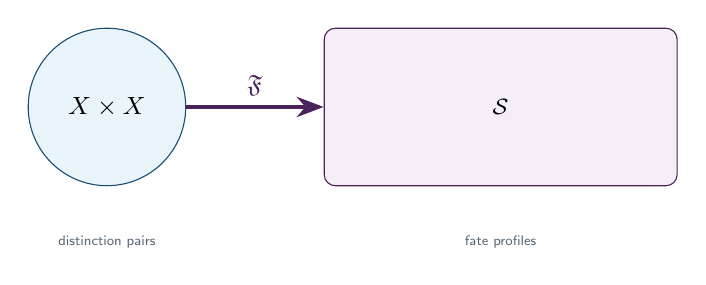
\begin{tikzpicture}
  \node[distnode,minimum size=2cm](D)at(0,0)
    {$\distPairs$};
  \node[fatenode,minimum size=2cm](S)at(5,0)
    {$\fateSpace$};
  \draw[fateedge,line width=1.5pt](D)--(S)
    node[midway,above,font=\sffamily\small\color{FateViolet}]
    {$\fateMap$};
  \node[below=0.5cm of D,font=\tiny\sffamily\color{DistGray}]
    {distinction pairs};
  \node[below=0.5cm of S,font=\tiny\sffamily\color{DistGray}]
    {fate profiles};
\end{tikzpicture}\\[2cm]
{\sffamily\color{DistGray}First Edition~·~2026}\\[0.5em]
{\sffamily\small\color{DistGray}
  Volume II of the Distinction Trilogy}
\end{titlepage}

% ---- Half-title with trilogy context -----------------------
\cleardoublepage
\vspace*{5cm}
\begin{center}
{\sffamily\large\color{DistGray}The Distinction Trilogy}\\[1em]
{\sffamily\normalsize\color{DistBlue}
  I.\quad Persistence Before Truth}\\[0.3em]
{\sffamily\normalsize\bfseries\color{FateViolet}
  II.\quad The Fate of Distinguishability}\\[0.3em]
{\sffamily\normalsize\color{DistBlue}
  III.\quad The Ecology of Distinctions}
\end{center}
\cleardoublepage

% ---- Table of contents -------------------------------------
\tableofcontents

% ---- Preface -----------------------------------------------
\chapter*{Preface: The Hinge Book}
\addcontentsline{toc}{chapter}{Preface}

This is the middle volume of a trilogy. The first volume,
\textit{Persistence Before Truth}, establishes why distinguishability
is necessary: if no distinctions survive or can be reconstructed
across transformation, then reference, measurement, communication,
and truth-evaluation all become impossible. The third volume,
\textit{The Ecology of Distinctions}, demonstrates what happens
when distinguishability operates in the wild: how distinctions
are born, how they die, how they compete, migrate, repair, and
regenerate across physical, biological, cognitive, and social
systems.

This volume asks the question that sits between those two:
\emph{what mathematical structures govern distinguishability?}

The primary object of study here is not a state, not an object,
not a memory, and not a proposition. It is a distinction pair
$(x,y)\in X\times X$ together with its \emph{fate}\ under
a family of operators. The fate map
$\fateMap:\distPairs\to\fateSpace$
assigns to each distinction pair a structured record of how it
fares under compression, forgetting, repair, transport, and
admissibility selection. Everything else in this volume is derived
from that object.

The central mathematical result is the Meta-Stability Theorem
(\cref{meta:meta-stability}): individual distinctions are not
conserved, but the operator algebra acting on them is. What
persists across all transformations is not any particular
distinction but the capacity to produce, destroy, and regenerate
distinguishability. This theorem is the formal answer to the
conservation question raised in \textit{Persistence Before
Truth\/} and the structural backbone underlying the population
dynamics of \textit{The Ecology of Distinctions}.

Readers of either outer volume will find that the concepts they
encountered there --- persistence, recoverability, repair,
admissibility, reachability, the preservation hierarchy --- all
appear here as special cases of a single operator-algebraic
framework. The goal is not to supersede those treatments but to
expose the formal skeleton they were always implicitly using.

\bigskip
\noindent\textit{How to read this book.}
Parts~I and~II establish the mathematical language. Part~III
develops the genuinely new material: fate geometry, fate
singularities, and the collapse stratum. Part~IV gives the
ecology dynamics in properly typed form. Part~V translates the
concepts of the outer volumes into fate-theoretic language.
Part~VI is the synthesis. A reader already fluent in
\textit{The Ecology of Distinctions\/} may enter at Part~III.
A reader coming from \textit{Persistence Before Truth\/} should
read Parts~I--III before skipping ahead.

\mainmatter

\part{Distinguishability Spaces}


% ============================================================
%  CHAPTER 1 — DISTINCTION PAIRS AND OBSERVATIONAL EQUIVALENCE
% ============================================================

\chapter{Distinction Pairs and Observational Equivalence}
\label{ch:distinction-pairs}

\begin{epigraph}{The world does not present itself as objects.
  It presents itself as differences.}{The founding observation}
\end{epigraph}

\begin{objectives}
\item Introduce distinction pairs as the primitive objects of
  the theory.
\item Explain why distinguishability is prior to classification.
\item Define observational families and observational equivalence.
\item Prove that observational equivalence is an equivalence
  relation and induces a partition of the state space.
\item Motivate the use of $X\times X$ rather than $X$ as the
  foundational domain.
\item Map the conceptual dependencies for the rest of the book.
\end{objectives}

\section{Why Begin With Distinctions?}

Most formal theories begin with objects. A set $X$ is given,
its elements are assumed to be identifiable, and the theory
proceeds to study their properties and relations. This approach
conceals a prior question: how did the elements of $X$ become
identifiable in the first place?

Before an entity can be measured, classified, or named, it must
first be distinguishable from something else. Distinguishability
is therefore prior to objecthood. An object is not a primitive
of the world but a cognitive and operational achievement: it is
what remains stable enough to be treated as a unit.

This volume begins not with objects but with distinctions. The
primitive is not a state $x\in X$ but a pair $(x,y)\in X\times X$
together with the information that $x$ and $y$ \emph{can be
told apart}. Everything else — objects, memories, persistence,
admissibility, knowledge, civilization — will be derived from
this starting point.

\section{State Spaces and Observation}

Let $X$ be a set whose elements represent possible states of a
system. The elements of $X$ are not assumed to be immediately
distinguishable. Distinguishability is conferred by observation.

\begin{definition}{Observational Family}{obs-family-ch1}
An \emph{observational family} is a collection
$\obs=\{o:X\to Y\}$ of maps from the state space into a
measurement space $Y$ equipped with a notion of equality.
Each $o\in\obs$ is an \emph{admissible observation}.
\end{definition}

An observational family encodes the set of measurements
available to an observer or system. Different choices of $\obs$
reflect different observational capabilities. The same pair of
states may be distinguishable under one family and
indistinguishable under another.

\section{Observational Equivalence}

\begin{definition}{Observational Equivalence}{obs-equiv-ch1}
Two states $x,y\in X$ are \emph{observationally equivalent}
with respect to $\obs$, written $x\sim_\obs y$, if
\[
  o(x) = o(y) \quad\text{for every }o\in\obs.
\]
A pair $(x,y)$ is \emph{operationally distinguishable} if
$x\not\sim_\obs y$.
\end{definition}

\begin{proposition}{Observational Equivalence is an Equivalence
  Relation}{obs-equiv-er-ch1}
The relation $\sim_\obs$ is reflexive, symmetric, and transitive.
\begin{proof}
Reflexivity: $o(x)=o(x)$ for every $o$.
Symmetry: if $o(x)=o(y)$ then $o(y)=o(x)$.
Transitivity: if $o(x)=o(y)$ and $o(y)=o(z)$ for every
$o\in\obs$, then $o(x)=o(z)$ for every $o\in\obs$.
All three hold for equality in $Y$.
\end{proof}
\end{proposition}

\begin{corollary}{Partition of the State Space}{state-partition}
The relation $\sim_\obs$ partitions $X$ into equivalence classes:
\[
  [x]_\obs \;=\; \{x'\in X : x'\sim_\obs x\}.
\]
The collection $\partitionObs = \{[x]_\obs : x\in X\}$ is the
\emph{observational partition} of $X$.
\end{corollary}

Each class in $\partitionObs$ contains states that cannot be
distinguished by any admissible observation. The partition
captures everything that is observationally accessible about
the state space structure.

\section{Why Pairs, Not States}

Traditional dynamical theories study the evolution of a single
state $x(t)\in X$. This approach is appropriate when the state
itself is the object of interest. But the questions driving
this volume are different:

Can this distinction \emph{survive} transformation?
Can it be \emph{repaired} after damage?
Can it be \emph{transported} to another context?
Does it \emph{collapse} under entropy?

None of these questions make sense for a single state. They
make sense for a \emph{pair} of states: a distinction consists
in the difference between $x$ and $y$, and it is the fate of
that difference that the theory studies.

The natural domain of fate theory is therefore not $X$ but
$\distPairs$.

\begin{definition}{Distinction Pair}{dist-pair-ch1}
A \emph{distinction pair} is an ordered pair
$(x,y)\in\distPairs$ such that $x\not\sim_\obs y$: some
admissible observation separates $x$ from $y$.
\end{definition}

The set of all distinction pairs is a subset of $\distPairs$
determined by $\obs$. The complement --- pairs $(x,y)$ with
$x\sim_\obs y$ --- are \emph{indistinguishable pairs}: states
the observation family cannot separate.

\begin{remark}{Objects as Derived Concepts}{objects-derived}
The theory does not deny the existence of objects. It derives
them. An object is what emerges when a collection of distinction
pairs is stable enough to be treated as a unit. Formally,
objects are equivalence classes of observationally
indistinguishable states: the elements of $\quotientObs$.
They are derived from the partition, not given in advance. This
derivation is made precise in Chapter~14.
\end{remark}

\section{What This Chapter Has Not Explained}

Several important questions are deferred to later chapters.

Chapter~2 asks: how is distinguishability measured? The answer
requires geometry on the pair space, developed via the
observational pseudometric.

Chapter~3 asks: how do distinctions behave under transformation?
The answer requires the survival ratio.

Chapters~5--9 ask: what are the operators that act on
distinctions? The answer requires the operator taxonomy.

Chapter~10 asks: what happens to a distinction in the long run?
The answer requires the fate map and the fate space.

\begin{chapsummary}
\item The primitive object of the theory is the distinction
  pair $(x,y)\in X\times X$, not the state $x\in X$.
\item Distinguishability is conferred by an observational
  family $\obs$ and is not intrinsic to the state space.
\item Observational equivalence $\sim_\obs$ is an equivalence
  relation partitioning $X$ into the observational partition
  $\partitionObs$.
\item Objects are derived as equivalence classes of
  indistinguishable states.
\item The remainder of the volume studies what happens to
  distinction pairs under transformation, operator action,
  and ecological dynamics.
\end{chapsummary}

% ============================================================
%  CHAPTER 2 — DISTINGUISHABILITY SPACES
% ============================================================

\chapter{Distinguishability Spaces}
\label{ch:dist-spaces}

\begin{epigraph}{A distinction is not merely present or absent.
  Distinctions possess geometry.}{The transition to measurement}
\end{epigraph}

\begin{objectives}
\item Define observational distance as a pseudometric on $X$.
\item Prove the triangle inequality from the metric on $Y$.
\item Characterize zero-distance pairs as exactly the
  observationally equivalent ones.
\item Show that the quotient $\quotientObs$ carries a genuine
  metric.
\item Define distinguishability capacity.
\item Prove capacity monotonicity under observational refinement.
\item Explain why capacity is the right static measure before
  dynamics are introduced.
\end{objectives}

Chapter~1 introduced observational equivalence as a binary
relation. Two states are either observationally equivalent or
they are not. Most real systems require a finer description:
some distinctions are robust, others fragile; some are
detectable by many observations, others only by one. The
purpose of this chapter is to quantify degrees of
distinguishability.

\section{Observational Distance}

Assume the measurement space $Y$ carries a metric $d_Y$.

\begin{definition}{Observational Distance}{obs-dist}
The \emph{observational distance} between $x,y\in X$ is
\[
  \distMetric(x,y)
  \;=\;
  \sup_{o\in\obs} d_Y(o(x),o(y)).
\]
\end{definition}

The observational distance measures the largest separability
achievable by any single admissible observation~\cite{shannon1948}. It represents
the maximum observational evidence available for distinguishing
the two states.

\begin{theorem}{Observational Distance is a Pseudometric}%
  {obs-pseudometric}
The function $\distMetric:X\times X\to\mathbb{R}_{\ge0}$ is a
pseudometric: non-negative, symmetric, satisfying the triangle
inequality, and zero on the diagonal.
\begin{proof}
\emph{Non-negativity}: $d_Y\ge 0$ so $\distMetric\ge 0$.

\emph{Symmetry}: $d_Y(o(x),o(y))=d_Y(o(y),o(x))$ for every
$o$, so $\distMetric(x,y)=\distMetric(y,x)$.

\emph{Triangle inequality}: for every $o\in\obs$ and every
$z\in X$,
\[
  d_Y(o(x),o(z))
  \;\le\;
  d_Y(o(x),o(y)) + d_Y(o(y),o(z))
  \;\le\;
  \distMetric(x,y) + \distMetric(y,z).
\]
Taking suprema over $o$:
$\distMetric(x,z)\le\distMetric(x,y)+\distMetric(y,z)$.

\emph{Diagonal}: $d_Y(o(x),o(x))=0$ for every $o$, so
$\distMetric(x,x)=0$.
\end{proof}
\end{theorem}

\begin{proposition}{Kernel Characterization}{kernel-char}
$\distMetric(x,y)=0$ if and only if $x\sim_\obs y$.
\begin{proof}
If $x\sim_\obs y$ then $o(x)=o(y)$ for every $o$, so every
term in the supremum is zero. Conversely, if
$\distMetric(x,y)=0$ then $d_Y(o(x),o(y))=0$ for every $o$,
hence $o(x)=o(y)$ for every $o$, i.e., $x\sim_\obs y$.
\end{proof}
\end{proposition}

The pseudometric fails to be a genuine metric precisely when
distinct states are observationally indistinguishable. This is
not a deficiency; it is the formal expression of the fundamental
fact that distinguishability depends on observation.

\section{The Metric Quotient}

\begin{theorem}{Metric on the Quotient}{metric-quotient}
The observational distance descends to a genuine metric
$\bar{d}_\obs$ on $\quotientObs$.
\begin{proof}
Define $\bar{d}_\obs([x],[y])=\distMetric(x,y)$. This is
well-defined because $\distMetric$ is constant on equivalence
classes: if $x\sim_\obs x'$ and $y\sim_\obs y'$ then
$o(x)=o(x')$ and $o(y)=o(y')$ for all $o$, so
$d_Y(o(x),o(y))=d_Y(o(x'),o(y'))$ for all $o$, hence
$\distMetric(x,y)=\distMetric(x',y')$.

The only metric axiom not inherited from $\distMetric$ is
$\bar{d}_\obs([x],[y])=0\Rightarrow [x]=[y]$. But
$\bar{d}_\obs([x],[y])=0$ means $\distMetric(x,y)=0$, which
by Proposition~\ref{prop:kernel-char} means $x\sim_\obs y$,
i.e., $[x]=[y]$.
\end{proof}
\end{theorem}

The metric space $(\quotientObs,\bar{d}_\obs)$ is the
\emph{distinguishability space} induced by $\obs$. It is the
geometric object that carries all observationally accessible
information about the state space.

\section{The Partition Lattice}

The observational partition $\partitionObs$ is one of many
possible partitions of $X$. Comparing partitions is natural:
one partition may be finer than another.

\begin{definition}{Refinement}{refinement-ch2}
A partition $\Pi_1$ \emph{refines} $\Pi_2$, written
$\Pi_1\preceq\Pi_2$, if every block of $\Pi_1$ is contained
in some block of $\Pi_2$.
\end{definition}

\begin{theorem}{Partitions Form a Lattice}{partition-lattice}
The set of all partitions of $X$ is a lattice under $\preceq$:
any two partitions have a greatest lower bound (common
refinement) and a least upper bound (coarsest common
coarsening).
\begin{proof}
Given $\Pi_1,\Pi_2$: their meet is the partition whose blocks
are all non-empty sets of the form $B_1\cap B_2$ with
$B_i\in\Pi_i$ --- the common refinement. Their join is the
partition generated by $\Pi_1\cup\Pi_2$ under transitivity
of block intersection --- the coarsest common coarsening. Both
constructions produce valid partitions, giving the lattice.
\end{proof}
\end{theorem}

\begin{theorem}{Refinement Monotonicity}{refinement-mono}
If $\obs_1\subseteq\obs_2$ then
$\partitionObs[_{\obs_2}]\preceq\partitionObs[_{\obs_1}]$:
a larger observational family induces a finer partition.
\begin{proof}
If $x\sim_{\obs_2}y$ then $o(x)=o(y)$ for every
$o\in\obs_2\supseteq\obs_1$, hence in particular for every
$o\in\obs_1$, so $x\sim_{\obs_1}y$. Every
$\sim_{\obs_2}$-class is contained in a $\sim_{\obs_1}$-class.
\end{proof}
\end{theorem}

\section{Distinguishability Capacity}

\begin{definition}{Distinguishability Capacity}{capacity-ch2}
For a finite state space $X$, the \emph{distinguishability
capacity} is
\[
  \capObs{X} \;=\; \log|\quotientObs|,
\]
the logarithm of the number of observationally distinguishable
categories.
\end{definition}

Capacity is the information-theoretic measure of observational
resolution. It counts how many operationally distinct things
can be told apart.

\begin{theorem}{Capacity Bounds}{capacity-bounds}
$0\le\capObs{X}\le\log|X|$.
\begin{proof}
$|\quotientObs|\ge 1$ (at least one class) and
$|\quotientObs|\le|X|$ (at most one class per state).
\end{proof}
\end{theorem}

\begin{theorem}{Capacity Monotonicity}{capacity-mono}
If $\obs_1\subseteq\obs_2$ then $\capObs[_{\obs_1}]{X}\le
\capObs[_{\obs_2}]{X}$.
\begin{proof}
By Refinement Monotonicity, $\Pi_{\obs_2}$ is finer than
$\Pi_{\obs_1}$, so $|\quotientObs[_{\obs_2}]|\ge
|\quotientObs[_{\obs_1}]|$. Applying $\log$ preserves the
inequality.
\end{proof}
\end{theorem}

\begin{remark}{Why Only a Static Measure}{static-capacity}
Capacity characterizes the observational resolution of the
current state but says nothing about what \emph{happens} to
distinctions under transformation. Two systems with the same
capacity may differ completely in how that capacity behaves
over time: one may maintain it, the other may lose it rapidly.
The theory of how capacity evolves under transformation begins
in Chapter~3.
\end{remark}

\begin{chapsummary}
\item The observational distance $\distMetric(x,y)=\sup_{o\in\obs}
  d_Y(o(x),o(y))$ is a pseudometric on $X$.
\item Zero distance corresponds exactly to observational
  equivalence: $\distMetric(x,y)=0$ iff $x\sim_\obs y$.
\item The quotient $(\quotientObs,\bar{d}_\obs)$ is a genuine
  metric space: the distinguishability space.
\item Observational partitions form a lattice under refinement;
  larger observation families produce finer partitions.
\item Distinguishability capacity $\capObs{X}=\log|\quotientObs|$
  measures observational resolution.
\item Capacity is monotone: more observations yield more
  capacity.
\item Capacity is a static measure; Chapter~3 introduces
  the dynamics.
\end{chapsummary}

% ============================================================
%  CHAPTER 3 — TRANSFORMATION CLASSES AND SURVIVAL
% ============================================================

\chapter{Transformation Classes and Survival}
\label{ch:transformation-survival}

\begin{epigraph}{A distinction that exists only momentarily is
  not yet part of the world.}{Persistence as a geometric
  property}
\end{epigraph}

\begin{objectives}
\item Introduce transformation families as the dynamical input.
\item Define distinction survival and the survival set.
\item Define the survival ratio $\survRatio_\transfam(x,y)$.
\item Prove that survival ratios lie in $[0,1]$.
\item Prove that invariant distinctions have unit survival ratio.
\item Show that survival is weaker and more general than
  invariance.
\item Identify the survival ratio as the first coordinate of
  the fate space (deferred to Chapter~10).
\end{objectives}

Chapters~1 and~2 established the geometry of distinguishability
at a single instant. Chapter~3 introduces time: transformation
families that act on the state space, and the question of
whether distinctions survive their action.

\section{Transformation Families}

\begin{definition}{Transformation Family}{trans-family-ch3}
A \emph{transformation family} is a measurable collection
$\transfam=\{T:X\to X\}$ of maps on the state space,
equipped with a probability measure $\mu$ on $\transfam$.
The measure $\mu$ weights the relative likelihood of each
transformation occurring.
\end{definition}

Examples include physical time evolution (where $\transfam$ is
a one-parameter group), stochastic degradation (where $\mu$
weights random perturbations), communication channels (where
each $T$ models a possible transmission error), and biological
mutation (where $\mu$ weights mutation rates).

\section{Distinction Survival}

\begin{definition}{Surviving Transformation}{surviving-T}
A transformation $T\in\transfam$ \emph{preserves} the
distinction $(x,y)$ if $T(x)\not\sim_\obs T(y)$: the
transformed states remain operationally distinguishable.
\end{definition}

\begin{definition}{Survival Set}{survival-set-ch3}
The \emph{survival set} of a distinction pair $(x,y)$ under
$\transfam$ is
\[
  \survivalSet{x,y}
  \;=\;
  \{T\in\transfam : T(x)\not\sim_\obs T(y)\}.
\]
\end{definition}

The survival set contains every transformation that preserves
the distinction. Its size, relative to the full transformation
family, measures robustness.

\section{The Survival Ratio}

\begin{definition}{Survival Ratio}{surv-ratio-ch3}
The \emph{survival ratio} of a distinction pair is
\[
  \survRatio_\transfam(x,y)
  \;=\;
  \frac{\mu(\survivalSet{x,y})}{\mu(\transfam)}.
\]
\end{definition}

The survival ratio is the probability that a randomly chosen
admissible transformation preserves the distinction. It
quantifies persistence as a measurable property rather than a
binary fact.

\begin{theorem}{Survival Ratio Bounds}{surv-bounds}
$0\le\survRatio_\transfam(x,y)\le 1$ for every distinction pair.
\begin{proof}
$\survivalSet{x,y}\subseteq\transfam$, so
$\mu(\survivalSet{x,y})\le\mu(\transfam)$. Non-negativity
of $\mu$ gives the lower bound.
\end{proof}
\end{theorem}

\begin{definition}{Complete Collapse and Perfect Persistence}%
  {extreme-surv}
A distinction pair has \emph{complete collapse} if
$\survRatio_\transfam(x,y)=0$: no admissible transformation
preserves it. It has \emph{perfect persistence} if
$\survRatio_\transfam(x,y)=1$: every admissible transformation
preserves it.
\end{definition}

\section{Invariance and Survival}

\begin{theorem}{Invariant Distinctions Have Unit Survival}%
  {invariant-unit}
If $T(x)\not\sim_\obs T(y)$ for every $T\in\transfam$, then
$\survRatio_\transfam(x,y)=1$.
\begin{proof}
The hypothesis means $\survivalSet{x,y}=\transfam$, so
$\mu(\survivalSet{x,y})=\mu(\transfam)$, giving $\survRatio=1$.
\end{proof}
\end{theorem}

The converse is not true in general: $\survRatio=1$ holds when
the survival set has full measure, which allows exceptional
transformations of measure zero to destroy the distinction.

\begin{remark}{Survival is Weaker Than Invariance}%
  {surv-vs-inv}
Invariance requires exact preservation under every
transformation. Survival requires only that the distinction
remain recoverable under a measure-$1$ set of transformations.

A repaired memory is not identical to its original encoding.
A translated sentence is not syntactically identical to the
original. A regenerated tissue is not molecularly identical
to its predecessor. Yet all may survive: the distinction
between them and the alternative remains operationally
accessible after reconstruction~\cite{spencerbrown1969}.

Persistence theory therefore studies recoverability rather
than invariance. This distinction is the conceptual foundation
of the repair theory developed in Chapter~7.
\end{remark}

\section{Survival as a Field on Pair Space}

The survival ratio defines a function
\[
  \survRatio_\transfam:\distPairs\to[0,1].
\]
This is the first coordinate of the fate space introduced in
Chapter~10. Two additional coordinates ($\repEff$ and
$\boldsymbol{\tau}$) and the collapse indicator $\collapseInd$
will be added there to complete the fate profile. The survival
ratio is where the geometry of fate begins.

\begin{remark}{What Survival Does Not Capture}%
  {surv-limits}
The survival ratio measures resistance to transformation. It
does not measure recoverability after damage: two distinctions
with identical survival ratios may differ completely in whether
they can be reconstructed after a transformation does destroy
them. That additional structure --- repair efficiency --- is
the subject of Chapter~7 and the second coordinate of the fate
space.
\end{remark}

\begin{chapsummary}
\item A transformation family $\transfam$ is a measurable~\cite{katok1995}
  collection of maps on $X$, with probability measure $\mu$.
\item A transformation preserves a distinction if the
  transformed pair remains operationally distinguishable.
\item The survival set $\survivalSet{x,y}$ contains the
  preserving transformations.
\item The survival ratio $\survRatio_\transfam(x,y)\in[0,1]$
  quantifies robustness.
\item Invariant distinctions have unit survival ratio; the
  converse holds only up to measure zero.
\item Survival is weaker than invariance: it requires
  recoverability, not exact preservation.
\item The survival ratio is the first coordinate of the fate
  map defined in Chapter~10.
\end{chapsummary}

% ============================================================
%  CHAPTER 4 — CAPACITY AND THE PARTITION LATTICE
% ============================================================

\chapter{Capacity and the Partition Lattice}
\label{ch:capacity}

\begin{epigraph}{Every observation partitions the world.
  Capacity measures how many pieces remain.}{Resolution and
  information}
\end{epigraph}

\begin{objectives}
\item Revisit distinguishability capacity as the capstone of
  Part~I's static theory.
\item Show that collapse, repair, and transport correspond to
  downward, upward, and lateral movements in the partition
  lattice.
\item Prove that the partition lattice is the wrong object for
  a dynamic theory --- motivating the operator framework of
  Part~II.
\item Introduce capacity as a conserved potential that
  operators act upon.
\item Bridge from partition geometry to operator algebra.
\end{objectives}

Parts~I's first three chapters introduced distinction pairs
(Chapter~1), their geometry (Chapter~2), and their survival
under transformation (Chapter~3). This chapter closes Part~I
by situating capacity and the partition lattice as the static
substrate upon which Part~II's operator theory will act.

\section{Capacity as Observational Resolution}

The distinguishability capacity $\capObs{X}=\log|\quotientObs|$
from Chapter~2 measures how many operationally distinct
categories exist relative to a given observation family. It is
a property of the pair $(\obs, X)$, not of any individual
distinction.

Capacity has a natural interpretation in information theory:
it is the maximum number of bits needed to identify a state
up to observational equivalence. A system with capacity $k$
requires $k$ binary observations to fully classify its states.

\section{Partition Dynamics}

The partition lattice is not merely a static structure.
Transformations and operators move systems through it.

\begin{definition}{Partition Dynamics}{partition-dynamics}
Three fundamental motions act on the partition lattice:
\begin{enumerate}[nosep,label=(\roman*)]
\item \emph{Collapse}: merging of partition blocks, moving
  the partition downward (toward coarser partitions) and
  decreasing capacity.
\item \emph{Repair}: splitting of partition blocks, moving the
  partition upward (toward finer partitions) and increasing
  capacity.
\item \emph{Transport}: relabeling of partition blocks without
  changing their structure, moving laterally through the
  lattice without changing capacity.
\end{enumerate}
\end{definition}

\begin{proposition}{Partition Motion Classification}%
  {partition-motion}
Every admissible operator acts on the partition lattice as one
of: collapse (downward), repair (upward), transport (lateral),
or a composition of these.
\begin{proof}
An operator $F$ on $X$ induces a partition $\Pi_F$ on $X$ via
the equivalence $x\sim_F y\Leftrightarrow F(x)\sim_\obs F(y)$.
If $\Pi_F\preceq\partitionObs$, the operator coarsens the
partition: collapse. If $\partitionObs\preceq\Pi_F$, the
operator refines: repair. If the induced partition is
isomorphic to $\partitionObs$ under a relabeling: transport.
Every operator falls into one of these cases or is a
composition.
\end{proof}
\end{proposition}

\section{Capacity as Conserved Potential}

Capacity is not generally conserved under operator action.
Collapse destroys capacity; repair creates capacity. But
capacity serves as a useful potential function tracking the
health of the distinction structure.

\begin{theorem}{Collapse Decreases Capacity}{collapse-cap}
Every collapse operator decreases or preserves capacity:
$C_\obs(\collapOp(X))\le\capObs{X}$.
\begin{proof}
Collapse coarsens $\partitionObs$, reducing the number of
blocks: $|\Pi_{\obs}(\collapOp(X))|\le|\quotientObs|$.
Taking logs preserves the inequality.
\end{proof}
\end{theorem}

\begin{theorem}{Repair Increases Capacity}{repair-cap}
Every repair operator increases or preserves capacity:
$C_\obs(\repair(X))\ge\capObs{X}$.
\begin{proof}
Repair refines $\partitionObs$ by splitting blocks:
$|\Pi_\obs(\repair(X))|\ge|\quotientObs|$. Taking logs.
\end{proof}
\end{theorem}

\section{Why the Partition Lattice Is Insufficient}

The partition lattice tells us \emph{what positions} a
distinction structure can occupy. It does not tell us:

\begin{itemize}[nosep,leftmargin=2em]
\item which operators are available to move between positions;
\item at what rate collapse or repair occurs;
\item whether a collapsed distinction can be recovered;
\item how distinctions survive repeated transformations;
\item which positions are admissible and which are excluded.
\end{itemize}

These questions require a theory of operators acting on
$\distPairs$, not just a theory of positions in the partition
lattice. Part~II develops that operator theory. Chapters~5--9
build the operator algebra needed to support the fate geometry
of Part~III.

\begin{trilogylink}{Capacity in the Outer Volumes}
In \textit{Persistence Before Truth}, capacity appears implicitly
as the condition under which truth-evaluation is possible: a
system needs sufficient observational resolution to distinguish
the states relevant to the propositions it evaluates.

In \textit{The Ecology of Distinctions}, capacity appears as
admissibility volume: the volume of the region of fate space
that a system can access. The Generative Admissibility
Principle says that admissible systems do not decrease this
volume.

In this volume, capacity is a derived quantity computed from
the observational partition. The Admissibility Pullback
Meta-Theorem (Chapter~13) shows that admissibility volume in
EOD is exactly the fate volume of this volume, connecting all
three treatments.
\end{trilogylink}

\begin{chapsummary}
\item Capacity $\capObs{X}=\log|\quotientObs|$ is the static
  measure of observational resolution established in
  Chapter~2.
\item Collapse, repair, and transport correspond to downward,
  upward, and lateral movements in the partition lattice.
\item Collapse decreases capacity; repair increases it;
  transport preserves it.
\item The partition lattice gives positions but not operators:
  it is the wrong object for a dynamic theory.
\item Part~II introduces the operator algebra that acts on the
  partition structure and provides the dynamic theory.
\end{chapsummary}

% ============================================================
%  CHAPTER 5 — A TAXONOMY OF DISTINGUISHABILITY OPERATORS
% ============================================================

\part{Operators on Distinguishability}
\chapter{A Taxonomy of Distinguishability Operators}
\label{ch:operator-taxonomy}

\begin{epigraph}{A geometry becomes a science only when we
  understand its transformations.}{Transition to operator
  theory}
\end{epigraph}

\begin{objectives}
\item Introduce operators acting on distinction pairs rather
  than states.
\item Define and separate the six fundamental operator classes.
\item Prove that the classes are non-empty and distinct.
\item Introduce the operator space $\distOp$.
\item Motivate the algebraic structure developed in
  Chapters~6--9.
\end{objectives}

Part~I established the geometry of distinguishability. We have:
$\distPairs$ (the domain), $\distMetric$ (the pseudometric),
$\survRatio_\transfam$ (the survival ratio), and $\partitionObs$
(the partition lattice). These structures describe distinctions.
They do not describe what acts upon distinctions.

Part~II studies operators: maps from distinction pairs to
distinction pairs that change, preserve, destroy, or restore
distinguishability. The central insight is that the operator
acts on $\distPairs$, not on $X$. State-space dynamics and
distinguishability dynamics are different theories acting on
different domains.

\section{Distinguishability Operators}

\begin{definition}{Distinguishability Operator}{dist-op-ch5}
A \emph{distinguishability operator} is a map
$F:\distPairs\to\distPairs$ acting on distinction pairs.
The \emph{operator space} is $\distOp=\{F:\distPairs\to
\distPairs\}$.
\end{definition}

This definition is deliberately broad. Operators need not be
bijective, continuous, or structure-preserving in any
particular sense. The taxonomy below classifies them by their
effect on distinguishability.

\section{The Six Fundamental Classes}

\begin{definition}{Fundamental Operator Classes}{op-classes}
A distinguishability operator $F\in\distOp$ belongs to one of
six classes according to its effect on $\distMetric$:
\begin{enumerate}[nosep,label=(\roman*)]
\item \emph{Preservation operators}: $\distMetric(F(x),F(y))=
  \distMetric(x,y)$ for all pairs --- exact isometry.
\item \emph{Collapse operators}: some $x\not\sim_\obs y$ maps
  to $F(x)\sim_\obs F(y)$ --- active reduction of distinction.
\item \emph{Forgetting operators}: collapse operators for
  which no admissible repair operator exists to recover the
  lost distinction.
\item \emph{Repair operators}: $\distMetric(F(x),F(y))\ge
  \distMetric(x,y)$ for damaged pairs --- restoration of
  distinguishability.
\item \emph{Transport operators}: isometries that relocate
  the distinction: $\distMetric(F(x),F(y))=\distMetric(x,y)$
  via a change of context.
\item \emph{Admissibility operators}: projections
  $\pi_A:\distPairs\to\distPairs$ restricting to pairs whose
  fate profile lies in an admissible region $A$.
\end{enumerate}
\end{definition}

\begin{theorem}{The Six Classes are Non-Empty and Distinct}%
  {classes-distinct}
Each of the six classes contains at least one operator not in
any other class.
\begin{proof}
\emph{Existence}:
(i) Identity is a preservation operator.
(ii) The projection $\pi:X\to\{*\}$ (collapsing all states)
  induces a collapse operator with $\distMetric=0$ everywhere.
(iii) Irreversible information erasure (e.g., overwriting memory
  with noise) gives a forgetting operator.
(iv) Any error-correcting decoder acting on a noisy copy is a
  repair operator: it increases $\distMetric$ of the repaired
  pair above the noisy copy's distance.
(v) A lossless communication channel: $F(x)=\phi(x)$ for a
  bijection $\phi$ preserving $\distMetric$ but changing context.
(vi) $\pi_A$ as defined above.

\emph{Distinctness}:
Collapse operators and repair operators have opposite effects
on $\distMetric$: the former decreases it, the latter increases
it. Transport operators preserve $\distMetric$ but change
context, while preservation operators preserve $\distMetric$
without changing context. Forgetting operators are a subclass
of collapse operators not reachable by repair. Admissibility
operators are selection operators not reducible to
collapse or repair. Hence no class reduces to another.
\end{proof}
\end{theorem}

\section{The Collapse--Forgetting Distinction}

The most important distinction within the taxonomy is between
collapse and forgetting, developed fully in Chapter~6.

Collapse is the loss of operational distinguishability. It is
potentially reversible: the distinction exists latently and may
be recovered by an appropriate repair operator.

Forgetting is the loss of the reconstruction pathway itself.
It is not reversible by any admissible operator: there is no
information remaining from which the lost distinction could be
recovered.

\begin{proposition}{Forgetting Implies Collapse}%
  {forget-implies-collapse}
Every forgetting operator is a collapse operator.
The converse fails.
\begin{proof}
A forgetting operator removes operational distinguishability,
so it is by definition a collapse operator. For the
converse: lossless compression collapses distinctions (the
compressed representation cannot immediately separate $x$ and
$y$) but retains the decompression pathway, so it is
recoverable collapse but not forgetting.
\end{proof}
\end{proposition}

\section{Operator Composition and Structure}

Operators compose: if $F,G\in\distOp$ then $G\circ F\in\distOp$.
Composition is the primary operation of Part~II.

Chapter~6 shows that forgetting operators form a proper
submonoid of collapse operators under composition.
Chapter~7 shows that repair operators are not generally
closed under composition but that their interaction with
collapse operators is central.
Chapter~8 shows that the full operator space $(\distOp,\circ,
\mathrm{Id})$ is a monoid.
Chapter~9 proves the Meta-Stability Theorem: the monoid
structure is the conserved object, even when individual
distinctions are not.

\begin{chapsummary}
\item Distinguishability operators act on $\distPairs$, not
  on $X$: the domain of fate theory differs from the domain
  of state-space dynamics.
\item Six classes: preservation, collapse, forgetting, repair,
  transport, admissibility.
\item The classes are non-empty, distinct, and cannot be
  reduced to one another.
\item Collapse and forgetting are not identical: forgetting
  adds loss of reconstruction pathways to collapse.
\item Operator composition structures Part~II.
\end{chapsummary}

% ============================================================
%  CHAPTER 6 — COLLAPSE AND FORGETTING
% ============================================================

\chapter{Collapse and Forgetting}
\label{ch:collapse-forgetting}

\begin{epigraph}{Not every disappearance is destruction.
  Not every destruction is forgetfulness.}{The distinction
  this chapter establishes}
\end{epigraph}

\begin{objectives}
\item Define collapse operators formally as partition-coarsening
  maps.
\item Define forgetting operators as the irrecoverable subclass
  of collapse.
\item Prove the Compression Fiber Theorem: collapse destroys
  exactly the distinctions within the fibers of the compressing
  map.
\item Prove that forgetting operators form a submonoid under
  composition.
\item Derive the diffusion monotonicity theorem as the canonical
  physical instance of collapse.
\item Introduce entropy as the geometry of distinction loss.
\item Distinguish collapse cascades from isolated collapse
  events.
\end{objectives}

Chapter~5 introduced collapse and forgetting as two of the six
operator classes. This chapter develops them in detail, proves
their key properties, and identifies the physical and
mathematical mechanisms through which distinctions are lost.

The chapter is where the framework first becomes irreversible.
Parts~I--II up to this point have been reversible in spirit:
operators could be studied without committing to a direction of
time. Collapse and forgetting introduce genuine irreversibility:
some distinction losses cannot be undone.

\section{Collapse as Compression}

\begin{definition}{Compression Map}{compression-map}
A \emph{compression map} is a surjective map
$\pi:X\to Q$ from the state space to a quotient space. It
induces an equivalence relation $x\sim_\pi y\Leftrightarrow
\pi(x)=\pi(y)$ and partitions $X$ into the \emph{fibers}
$\pi^{-1}(q)$ for $q\in Q$.
\end{definition}

\begin{theorem}{Compression Fiber Theorem}{compression-fiber}
A compression map $\pi:X\to Q$ destroys exactly the
distinctions within its fibers:
\[
  L_\pi
  \;=\;
  \{(x,y)\in\distPairs : x\not\sim_\obs y,\; x\sim_\pi y\}
\]
is the set of destroyed distinctions.
\begin{proof}
If $\pi(x)=\pi(y)$ (same fiber), then no observation in $Q$
can separate $\pi(x)$ from $\pi(y)$, so the compressed
representation cannot separate $x$ from $y$: the distinction
is lost.

If $\pi(x)\neq\pi(y)$ (different fibers), then the
compression preserves their separation in $Q$: the distinction
survives.

Hence the destroyed distinctions are precisely those in
$L_\pi$.
\end{proof}
\end{theorem}

\begin{corollary}{Collapse Decreases Capacity}{collapse-cap-ch6}
For any compression $\pi$, $\capObs{\pi(X)}\le\capObs{X}$,
with equality iff $\pi$ is injective (no fibers merge).
\begin{proof}
The number of distinguishable classes in $\pi(X)$ cannot
exceed that in $X$.
\end{proof}
\end{corollary}

\section{Forgetting: Collapse Plus Loss of Pathways}

\begin{definition}{Forgetting Operator}{forget-op-ch6}
A collapse operator $\forgetOp$ is a \emph{forgetting
operator} if no admissible repair operator $R\in\distOp$
satisfies $R\circ\forgetOp(x)\not\sim_\obs R\circ\forgetOp(y)$
for all $(x,y)\in L_{\forgetOp}$: the lost distinctions cannot
be recovered by any admissible operator.
\end{definition}

\begin{theorem}{Forgetting Submonoid}{forget-monoid}
The class of forgetting operators is closed under composition:
if $\forgetOp_1$ and $\forgetOp_2$ are forgetting operators,
then $\forgetOp_2\circ\forgetOp_1$ is a forgetting operator.
\begin{proof}
$\forgetOp_1$ destroys distinctions in $L_{\forgetOp_1}$
with no recovery pathway. $\forgetOp_2$ then acts on the
already-degraded structure, destroying further distinctions
in $L_{\forgetOp_2}$. The composite $\forgetOp_2\circ
\forgetOp_1$ destroys all distinctions in
$L_{\forgetOp_1}\cup\forgetOp_1^*(L_{\forgetOp_2})$, where
$\forgetOp_1^*$ denotes the pushforward. Since no recovery
pathway existed for $L_{\forgetOp_1}$, and $\forgetOp_2$
removes further pathways, no admissible repair operator
can recover the composite loss. Hence the composition
is a forgetting operator. Together with the identity
(trivial forgetting), this gives the submonoid.
\end{proof}
\end{theorem}

\section{Diffusion as Canonical Collapse}

Physical diffusion provides the canonical example of a collapse
operator: it monotonically destroys the observational
separation between field configurations.

\begin{theorem}{Diffusion Decreases Distinguishability}%
  {diffusion-mono}
Let $u,v$ be two field configurations evolving under diffusion
$\partial_t u = D\nabla^2 u$, $\partial_t v = D\nabla^2 v$.
Define the distinguishability energy
$\repEng(t)=\int_\Omega |u(x,t)-v(x,t)|^2\,dx$.
Then $\dot{\repEng}(t)\le 0$: distinguishability is
non-increasing under diffusion.
\begin{proof}
Let $w=u-v$. Then $\partial_t w=D\nabla^2 w$.
\begin{align*}
  \dot{\repEng}
  &= 2\int_\Omega w\,\partial_t w\,dx
  = 2D\int_\Omega w\nabla^2 w\,dx \\
  &= -2D\int_\Omega |\nabla w|^2\,dx \;\le\; 0,
\end{align*}
where the last step uses integration by parts with vanishing
boundary conditions.
\end{proof}
\end{theorem}

Diffusion acts as a continuous collapse operator: the integral
$\int|\nabla w|^2$ measures the spatial variation of the
distinction, and its positivity drives $\repEng$ downward.

\section{Entropy as the Geometry of Distinction Loss}

Collapse has an informational signature: it maps many
distinguishable states into the same observational category,
increasing the \emph{representational entropy} of the system.

\begin{definition}{Representational Entropy}{rep-entropy-ch6}
Let $\pi:X\to\quotientObs$ be the observational projection.
The \emph{representational entropy} at a point $q\in\quotientObs$
is
\[
  \repEntropy(q)
  \;=\;
  \log\Vol\bigl(\pi^{-1}(q)\bigr),
\]
the logarithm of the volume of the indistinguishable fiber.
\end{definition}

Collapse enlarges fibers: $\Vol(\pi^{-1}(q))$ increases as
distinctions are merged~\cite{shannon1948}. Therefore collapse increases
representational entropy --- the observationally equivalent
states become more numerous. This foreshadows the connection
to fate entropy established in Chapter~15D, where entropy is
defined as the rate of contraction of the reachable fate volume.

\section{Collapse Cascades}

Individual collapses rarely occur in isolation. The loss of
one distinction often reduces the survival ratio of neighboring
distinctions, making cascade more likely.

\begin{definition}{Collapse Cascade}{collapse-cascade-ch6}
A \emph{collapse cascade} is a sequence
$\collapOp_1,\collapOp_2,\ldots,\collapOp_n$ of collapse
operators such that the action of $\collapOp_i$ increases
the collapse rate of $\collapOp_{i+1}$: the distinctions
destroyed by $\collapOp_i$ were supporting the stability
of the distinctions targeted by $\collapOp_{i+1}$.
\end{definition}

Collapse cascades appear throughout the trilogy: ecosystem
collapse (Chapter~18), paradigm shifts (Chapter~17),
institutional failure (Chapter~21), and language extinction
(Chapter~18). They all share the same structural signature:
each collapse event reduces the repair capacity of neighboring
distinctions, accelerating subsequent collapse.

\section{The Repair Dual}

Every collapse operator has a natural dual question: can the
loss be reversed? If so, how? If not, why not?

The answers to these questions constitute repair theory, the
subject of Chapter~7. Repair and collapse are not merely
opposites: they operate under different constraints, have
different efficiency measures, and interact in non-commutative
ways (Chapter~8's operator algebra). But understanding collapse
fully requires understanding its relationship to repair.

\begin{chapsummary}
\item Collapse operators coarsen the observational partition,
  destroying distinctions within the fibers of a compression
  map.
\item The Compression Fiber Theorem: exactly the fiber-internal
  distinctions are destroyed.
\item Forgetting operators are collapse operators with no
  admissible recovery pathway; they form a submonoid under
  composition.
\item Diffusion is the canonical physical collapse operator:
  distinguishability energy $\repEng(t)$ is non-increasing.
\item Representational entropy increases under collapse:
  fibers grow larger.
\item Collapse cascades occur when distinction loss reduces
  the repair capacity of neighboring distinctions.
\end{chapsummary}



% ============================================================
%  CHAPTER 7 — REPAIR AND TRANSPORT
% ============================================================

\chapter{Repair and Transport}
\label{ch:repair-transport}

\begin{epigraph}{Not every loss is permanent. Not every change
  destroys. The dual of collapse is not just absence of collapse
  --- it is active regeneration and continuation.}{The operators
  this chapter studies}
\end{epigraph}

\begin{objectives}
\item Define repair operators as active restoration of
  distinguishability after damage.
\item Prove that repair efficiency $\repairEff{x,y}\in[0,1]$
  is bounded and well-defined.
\item Show that repair is not restoration to identity but
  restoration of recoverability.
\item Define transport operators as isometries that relocate
  distinctions without destroying them.
\item Prove the Repair--Transport Duality: the two operator
  classes are complementary in their action on the fate
  coordinates $(\survRatio, \repEff, \boldsymbol{\tau})$.
\item Show that repair and transport are not commutative with
  collapse.
\item Prepare the transition to the operator monoid of
  Chapter~8.
\end{objectives}

Chapter~6 showed how distinctions are lost: through collapse
(partition coarsening) and forgetting (loss of reconstruction
pathways). This chapter shows how they are maintained and
propagated: through repair (restoration of recoverability
after damage) and transport (structure-preserving relocation).

Repair and transport are not simply the absence of collapse.
They are active operators with their own algebraic properties,
their own efficiency measures, and their own interaction
patterns with the collapse operators of Chapter~6. Together,
collapse-forgetting and repair-transport are the two poles of
the distinction lifecycle.

\section{Repair: Restoring Recoverability}

Repair is the active restoration of distinguishability after
a degrading transformation has reduced it. The key insight,
already visible in \PBT{Chapter~4}, is that repair need not
reconstruct the original state. It need only reconstruct the
distinction: restore operational separability between $x$ and
$y$.

\begin{definition}{Degradation--Repair Pair}%
  {degrade-repair-pair}
A \emph{degradation--repair pair} $(\degradeOp, R)$ consists
of a degradation operator $\degradeOp:\distPairs\to\distPairs$
and a repair operator $R:\distPairs\to\distPairs$ such that
for all $(x,y)\in\distPairs$:
\[
  \distMetric(\degradeOp(x),\degradeOp(y))
  \;\le\;
  \distMetric(x,y),
\]
i.e., $\degradeOp$ reduces observational distance (degrades
the distinction), while $R$ acts on the degraded output.
\end{definition}

\begin{definition}{Repair Efficiency}{repair-eff}
The \emph{repair efficiency} of a repair operator $R$ on
a degradation $\degradeOp$ is
\[
  \repairEff{x,y}
  \;=\;
  \frac{
    \distMetric\bigl(R(\degradeOp(x)),\,R(\degradeOp(y))\bigr)
  }{
    \distMetric(x,y)
  },
\]
where the denominator is the original distinguishability
before degradation. The repair efficiency measures the
fraction of original distinguishability restored by $R$
after $\degradeOp$.
\end{definition}

\begin{theorem}{Repair Efficiency is Bounded}{repair-eff-bounded}
Under the assumption that repair is \emph{non-amplifying}
--- it does not increase distinguishability beyond the original
level: $\distMetric(R(\degradeOp(x)),R(\degradeOp(y)))\le
\distMetric(x,y)$ --- the repair efficiency satisfies
$0\le\repairEff{x,y}\le 1$.
\begin{proof}
The numerator $\distMetric(R(\degradeOp(x)),R(\degradeOp(y)))$
is non-negative by the pseudometric axiom. Under the
non-amplifying assumption, it is also bounded above by
$\distMetric(x,y)$. Dividing by $\distMetric(x,y)>0$
gives $\repairEff{x,y}\in[0,1]$.
\end{proof}
\end{theorem}

\begin{remark}{Non-Amplification as Axiom}{non-amplify}
The non-amplifying assumption is stated explicitly as an axiom
rather than derived. It encodes the physical constraint that
repair cannot create distinguishability~\cite{friston2010} beyond what was present
originally: a repair operator cannot increase signal-to-noise
ratio above its pre-damage level without additional external
information. This assumption holds in all physical, biological,
and computational models of interest. Systems that violate it
--- which would require free information creation --- are
outside the scope of the present framework.
\end{remark}

\begin{definition}{Perfect Repair and Irreparable Damage}%
  {repair-extremes}
A distinction $(x,y)$ is \emph{perfectly repaired} if
$\repairEff{x,y}=1$: full distinguishability is restored.
It is \emph{irreparably damaged} if $\repairEff{x,y}=0$ for
all available $R$: the distinction lies in the forgetting
stratum $\strataF$ (Chapter~12).
\end{definition}

\section{Repair is Not Restoration}

A common misunderstanding identifies repair with restoration
to the original state. The present framework separates these.

\begin{proposition}{Repair Requires Only Recoverability, Not
  Identity}{repair-not-restore}
A repair $R$ is successful whenever
$\repairEff{x,y}>0$, regardless of whether
$R(\degradeOp(x))=x$ and $R(\degradeOp(y))=y$.
\begin{proof}
Success of repair is defined by restoration of operational
separability: $R(\degradeOp(x))\not\sim_\obs R(\degradeOp(y))$.
This holds whenever $\distMetric(R(\degradeOp(x)),R(\degradeOp(y)))>0$,
i.e., whenever $\repairEff{x,y}>0$. The condition does not
require $R(\degradeOp(x))=x$.
\end{proof}
\end{proposition}

This proposition has consequences throughout the trilogy. A
biological organism that repairs genetic damage need not
recreate the exact original sequence; it needs to restore
functional distinction between healthy and damaged phenotypes.
A memory that is reconstructed need not be pixel-perfect; it
needs to restore the distinction that matters for current
action. A scientific theory that is revised need not recover
its original formulation; it needs to restore the distinctions
between phenomena that the original theory drew.

\section{Transport: Structure-Preserving Relocation}

\begin{definition}{Transport Operator}{transport-op}
A \emph{transport operator} $\transpOp:\distPairs\to\distPairs$
is a map satisfying
\[
  \distMetric(\transpOp(x),\transpOp(y))
  \;=\;
  \distMetric(x,y)
\]
for all $(x,y)\in\distPairs$: transport is an isometry of the
observational pseudometric.
\end{definition}

Transport operators preserve the distinguishability distance
exactly. They change the context of the distinction --- its
location in some ambient space, its carrier medium, its
encoding --- without changing its magnitude.

\begin{example}{Canonical Transport Operators}%
  {transport-examples}
A lossless communication channel $\transpOp$ maps a sent
signal $(x,y)$ to a received signal $(\transpOp(x),\transpOp(y))$
with $\distMetric(\transpOp(x),\transpOp(y))=\distMetric(x,y)$:
the distinction between two signals is preserved across the
channel.

Genetic inheritance: a parent organism $(x,y)$ transmits
distinctions to offspring $(\transpOp(x),\transpOp(y))$
through replication, preserving the distinction between genetic
variants.

Cultural transmission: a distinction between two concepts in
one generation is transmitted to the next with full fidelity
by a transport operator (ideal education, scribal copying,
oral tradition under ideal conditions).
\end{example}

\begin{proposition}{Transport Operators Are Invertible Iff
  Bijective}{transport-invertible}
A transport operator $\transpOp$ is invertible (has an inverse
transport operator $\transpOp^{-1}$) if and only if $\transpOp$
is bijective on $\distPairs$.
\begin{proof}
An isometry of a metric space is invertible iff it is bijective:
the inverse of a distance-preserving bijection is itself
distance-preserving. The isometry condition
$\distMetric(\transpOp(x),\transpOp(y))=\distMetric(x,y)$
ensures the inverse preserves distance.
\end{proof}
\end{proposition}

\section{The Repair--Transport Duality}

Repair and transport are complementary operators, but their
complementarity is not simply ``repair is to collapse as
transport is to preservation.'' The duality is more structured:
repair and transport act on different coordinates of the future
fate profile.

\begin{proposition}{Repair--Transport Duality in Fate Coordinates}%
  {repair-transport-duality}
For a distinction pair $(x,y)$ with fate profile
$(\survRatio,\repEff,\collapseInd,\boldsymbol{\tau})$:
\begin{enumerate}[nosep,label=(\roman*)]
\item A repair operator $R$ acts primarily on $\repEff$:
  it increases the repair efficiency coordinate
  of the fate profile, while $\survRatio$ and
  $\boldsymbol{\tau}$ may vary independently.
\item A transport operator $\transpOp$ acts primarily on
  $\boldsymbol{\tau}$: it increases the transport-reach
  coordinates of the fate profile, while preserving
  $\distMetric$ (hence tending to preserve $\survRatio$
  and $\repEff$).
\item The two effects are independent: a distinction may have
  high repair efficiency and low transport reach, or vice
  versa, or both high, or both low.
\end{enumerate}
\begin{proof}
(i): Repair efficiency $\repEff=\repairEff{x,y}$ is by
definition the ratio of restored to original distance.
Repair directly increases this coordinate. The survival ratio
$\survRatio$ depends on the transformation family, not on $R$,
so it may vary independently.

(ii): Transport reach $\tau_i$ measures the distance over
which the distinction remains recoverable under the $i$-th
transport channel. Applying $\transpOp$ extends this reach.
The isometry condition $\distMetric(\transpOp(x),\transpOp(y))
=\distMetric(x,y)$ means $\survRatio$ and $\repEff$ are
preserved under ideal transport.

(iii): Consider a distinction that is easily repaired (high
$\repEff$) but cannot be transported beyond a small
neighborhood (low $\tau$): a biological immune memory that
is regenerated locally but not systematically communicated.
Conversely, consider a radio signal that propagates globally
(high $\tau$) but is easily jammed (low $\repEff$). These
examples demonstrate independence.
\end{proof}
\end{proposition}

\section{Non-Commutativity with Collapse}

Repair and transport do not commute with collapse. This
non-commutativity is not a deficiency of the algebra but a
reflection of the irreversibility of information loss.

\begin{theorem}{Repair and Collapse Do Not Generally Commute}%
  {repair-collapse-noncommute}
There exist operators $R$ (repair) and $\collapOp$ (collapse)
such that $R\circ\collapOp\neq\collapOp\circ R$ as operators
on $\distPairs$.
\begin{proof}
Take $\collapOp$ to be a compression that maps two
observationally distinct states to the same image:
$\collapOp(x)=\collapOp(y)$ with $x\not\sim_\obs y$.

$R\circ\collapOp$: collapse first, then repair. After collapse,
$\distMetric(\collapOp(x),\collapOp(y))=0$. If the repair
operator has no information about the pre-collapse distinction
(the typical case when the collapse is a forgetting operator),
then $R(\collapOp(x))=R(\collapOp(y))$ and no distinction is
restored.

$\collapOp\circ R$: repair first, then collapse. Since $R$
acts before collapse, it may restore or enhance the distinction.
Subsequent collapse then destroys a distinction that was larger
than the original.

The two orderings produce different results.
\end{proof}
\end{theorem}

The non-commutativity theorem has an immediate practical
consequence: the order of operations matters. Repairing before
collapse preserves more information than repairing after.
Archiving before disaster preserves more than archiving after.
Vaccinating before infection preserves more than treating after.
Chapter~8's operator algebra will capture this ordering
structure.

\section{Repair Chains and Efficiency Decay}

Real repair processes are rarely single operations. They
are chains: a sequence of repair operators applied iteratively.

\begin{proposition}{Repair Chain Efficiency}{repair-chain}
For a repair chain $R_n\circ R_{n-1}\circ\cdots\circ R_1$
applied after degradation $\degradeOp$, the net efficiency
satisfies
\[
  \eta_{R_n\circ\cdots\circ R_1}(x,y)
  \;\le\;
  \min_i \eta_{R_i}(x,y),
\]
where $\eta_{R_i}$ is the efficiency of $R_i$ at its stage
of the chain.
\begin{proof}
Each repair $R_i$ can at most restore to the level available
after the previous repairs: the efficiency of the chain is
bounded by the efficiency of its weakest link. Formally, the
distortion compounds: $\distMetric$ after $n$ repairs is at
most $\min_i \eta_{R_i}\cdot\distMetric(x,y)$ since each
$\eta_{R_i}\le 1$.
\end{proof}
\end{proposition}

\begin{chapsummary}
\item Repair operators restore distinguishability after
  degradation: $\repairEff{x,y}=\distMetric(R\circ D(x),
  R\circ D(y))/\distMetric(x,y)\in[0,1]$.
\item Repair requires recoverability, not identity: success
  means $\repairEff>0$, not $R\circ D=\mathrm{Id}$.
\item Transport operators are isometries: they preserve
  $\distMetric$ while relocating the distinction.
\item The Repair--Transport Duality: repair acts on $\repEff$,
  transport acts on $\boldsymbol{\tau}$; the two coordinates
  are independent.
\item Repair and collapse are non-commutative: order matters,
  and repair before collapse generally preserves more
  information.
\item Repair chains have efficiency bounded by the weakest
  link.
\end{chapsummary}

% ============================================================
%  CHAPTER 8 — THE DISTINGUISHABILITY OPERATOR MONOID
% ============================================================

\chapter{The Distinguishability Operator Monoid}
\label{ch:operator-monoid}

\begin{epigraph}{Individual distinctions may fail. The space
  of possible operations persists.}{Toward Meta-Stability}
\end{epigraph}

\begin{objectives}
\item Prove that $\distOp$ is closed under composition.
\item Establish associativity and the identity element.
\item Prove the Operator Closure Theorem: $(\distOp,\circ,
  \mathrm{Id})$ is a monoid.
\item Characterize the invertible subgroup and the
  non-invertible submonoid.
\item Show that collapse and forgetting form a proper
  submonoid.
\item Prepare the pullback construction of Chapter~9.
\end{objectives}

Chapters~5--7 introduced six classes of distinguishability
operators and studied their individual properties. This chapter
shows that these classes, taken together, form a coherent
algebraic object: the distinguishability operator monoid. This
is the algebraic structure that Chapter~9 will show to be
meta-stable.

\section{Composition of Operators}

\begin{definition}{Operator Composition}{op-comp}
For $F,G\in\distOp$, their \emph{composition} is the operator
$F\circ G:\distPairs\to\distPairs$ defined by
\[
  (F\circ G)(x,y) \;=\; F(G(x,y)).
\]
$G$ acts first, then $F$ acts on the output.
\end{definition}

\section{The Operator Closure Theorem}

\begin{theorem}{Operator Closure Theorem}{op-closure}
The collection $\distOp$ of all distinguishability operators
is closed under composition, contains an identity element,
and satisfies associativity. Therefore
$(\distOp,\circ,\mathrm{Id})$ is a monoid.
\begin{proof}
\emph{Closure}: if $F,G:\distPairs\to\distPairs$ then
$F\circ G:\distPairs\to\distPairs$ by function composition.
Hence $F\circ G\in\distOp$.

\emph{Associativity}: for any $F,G,H\in\distOp$ and any
$(x,y)\in\distPairs$,
\[
  ((F\circ G)\circ H)(x,y)
  = F(G(H(x,y)))
  = (F\circ(G\circ H))(x,y).
\]

\emph{Identity}: the identity operator $\mathrm{Id}(x,y)=(x,y)$
satisfies $F\circ\mathrm{Id}=F$ and $\mathrm{Id}\circ F=F$
for every $F\in\distOp$.

The three monoid axioms hold.
\end{proof}
\end{theorem}

\section{Invertible Operators and the Subgroup}

\begin{definition}{Invertible Operator}{invertible-op}
An operator $F\in\distOp$ is \emph{invertible} if there exists
$F^{-1}\in\distOp$ such that $F^{-1}\circ F=F\circ F^{-1}=
\mathrm{Id}$.
\end{definition}

\begin{theorem}{Invertible Operators Form a Group}{invertible-group}
The collection $\distOpInv$ of invertible operators forms a
group under composition.
\begin{proof}
$\distOpInv$ inherits closure (composition of invertibles is
invertible: $(F\circ G)^{-1}=G^{-1}\circ F^{-1}$),
associativity, and identity from $\distOp$. Every element has
an inverse by definition. Hence $\distOpInv$ is a group.
\end{proof}
\end{theorem}

\begin{proposition}{Transport Operators Generate Invertibles}%
  {transport-invertible-ch8}
Every bijective transport operator (Chapter~7) belongs to
$\distOpInv$.
\begin{proof}
A bijective isometry of $\distPairs$ has an inverse that is
also an isometry. Hence the inverse is a transport operator
in $\distOp$.
\end{proof}
\end{proposition}

\section{Non-Invertible Operators and the Submonoid}

\begin{theorem}{Non-Invertible Submonoid}%
  {noninv-submonoid}
The collection $\distOpNI$ of non-invertible operators forms
a proper submonoid of $(\distOp,\circ)$.
\begin{proof}
\emph{Closure}: if $F,G$ are non-invertible, we claim $F\circ G$
is non-invertible. Suppose for contradiction that $F\circ G$
is invertible with inverse $H$. Then $H\circ F\circ G=
\mathrm{Id}$, so $G$ has left inverse $H\circ F$ and is
right-invertible. But a non-invertible operator in the monoid
cannot be right-invertible (if $G$ had right inverse $K$ then
$G\circ K=\mathrm{Id}$, and left-composing by $H\circ F$
gives $K=H\circ F$, making $G$ invertible with inverse $K$ ---
a contradiction). Hence $F\circ G$ is non-invertible.

\emph{Proper}: bijective transport operators are invertible
and in $\distOp\setminus\distOpNI$.

\emph{Identity}: $\distOpNI$ does not contain $\mathrm{Id}$
(which is invertible). It is a sub-semigroup rather than a
submonoid in the strict sense; if we adjoin $\mathrm{Id}$, we
obtain a proper submonoid.
\end{proof}
\end{theorem}

\begin{remark}{Irreversibility as Algebraic Property}%
  {irreversibility-algebra}
The non-invertible submonoid $\distOpNI$ is the algebraic locus
of irreversibility. Collapse, forgetting, and non-bijective
transport operators all belong to it. The fact that $\distOpNI$
is closed under composition reflects the observation that
irreversibility compounds: applying two irreversible processes
in sequence produces an irreversible composite. This is the
algebraic counterpart of the thermodynamic statement that
entropy is non-decreasing in an isolated system.
\end{remark}

\section{The Collapse--Forgetting Submonoid}

\begin{proposition}{Collapse--Forgetting Submonoid}%
  {cf-submonoid}
The collection of collapse-and-forgetting operators forms a
proper submonoid of $\distOpNI$.
\begin{proof}
Collapse operators are closed under composition: composing two
operators that coarsen the observational partition produces
an operator that further coarsens it (since coarsening is
transitive in the partition lattice). Forgetting operators
are a subclass. The submonoid is proper because repair
operators are in $\distOp$ but not in this submonoid.
\end{proof}
\end{proposition}

\section{Operator Histories as Monoid Words}

A sequence of operator applications $F_n\circ\cdots\circ F_1$
is a \emph{word} in the monoid $\distOp$. The study of such
words is the study of operator histories: what sequence of
collapses, repairs, and transports has a distinction pair
experienced?

The monoid does not remember individual operators after
composition: only the cumulative action $F_n\circ\cdots\circ F_1$
is visible in the output. This motivates the next chapter's
question: what is preserved across all possible operator
histories?

\begin{chapsummary}
\item The Operator Closure Theorem: $(\distOp,\circ,\mathrm{Id})$
  is a monoid.
\item Invertible operators form a subgroup $\distOpInv$;
  bijective transport operators generate it.
\item Non-invertible operators form a proper submonoid
  $\distOpNI$: irreversibility is closed under composition.
\item Collapse and forgetting operators form a further proper
  submonoid.
\item An operator sequence $F_n\circ\cdots\circ F_1$ is a
  word in $\distOp$; its cumulative action on a distinction
  pair is the only observable output.
\end{chapsummary}

% ============================================================
%  CHAPTER 9 — THE META-STABILITY THEOREM
% ============================================================

\chapter{The Meta-Stability Theorem}
\label{ch:meta-stability}

\begin{epigraph}{Nothing guarantees the survival of a
  distinction. Something guarantees the survival of the
  possibility of distinction.}{The central discovery of
  Part~II}
\end{epigraph}

\begin{objectives}
\item Define the pullback induced action $T^*$ on $\distOp$
  and establish why this is the correct definition.
\item Prove that $T^*$ is a monoid homomorphism.
\item State and prove the Meta-Stability Theorem.
\item Identify the conserved object: the algebraic structure
  of $\distOp$, not any particular distinction.
\item Interpret the theorem at the physical, cognitive, and
  civilizational scales.
\item Explain why this theorem makes Chapter~10's Fate Space
  necessary.
\end{objectives}

Part~II has constructed the algebraic machinery: six operator
classes, their composition, the monoid $(\distOp,\circ,
\mathrm{Id})$, and the distinction between invertible and
non-invertible operators. The question this chapter answers is:
\emph{what survives the action of an admissible transformation
on this machinery?}

Individual distinctions clearly need not survive. Collapse
operators exist and destroy distinguishability. The question is
whether anything about the \emph{structure} of the operator
algebra is preserved.

\section{The Problem with Naive Induced Actions}

The natural first attempt at lifting a transformation $T$ to
an action on $\distOp$ is to define the pushforward:
$(T_*F)(x,y)=T(F(x,y))$. However, this definition does not
preserve composition:
\[
  T_*(F\circ G)(x,y)
  = T(F(G(x,y))),
\]
while
\[
  (T_*F)\circ(T_*G)(x,y)
  = T(F(T(G(x,y)))),
\]
and these are equal only when $T$ is the identity on
the range of $G$ --- a severely restrictive condition. The
pushforward is not a monoid homomorphism in general.

\section{The Pullback: The Correct Induced Action}

The correct definition uses the pullback rather than the
pushforward.

\begin{definition}{Pullback Induced Action}{pullback-action}
Let $T:X\to X$ be an admissible transformation. The
\emph{pullback action} of $T$ on $\distOp$ is the map
$T^*:\distOp\to\distOp$ defined by
\[
  (\pullback{T}{F})(x,y)
  \;=\;
  F\bigl(T(x),T(y)\bigr).
\]
The pullback first applies $T$ to both components of the
distinction pair, then applies $F$ to the transformed pair.
\end{definition}

The pullback has a clear interpretation: $\pullback{T}{F}$
is the operator $F$ as experienced by a distinction pair that
has already been transformed by $T$. It measures how $F$
acts on the $T$-image of the pair.

\section{The Pullback is a Monoid Homomorphism}

\begin{theorem}{Pullback Preserves Composition}%
  {pullback-comp}
For all $F,G\in\distOp$ and all admissible $T$:
\[
  \pullback{T}{(F\circ G)}
  \;=\;
  (\pullback{T}{F})\circ(\pullback{T}{G}).
\]
\begin{proof}
Evaluate both sides at $(x,y)\in\distPairs$:
\begin{align*}
  \bigl[\pullback{T}{(F\circ G)}\bigr](x,y)
  &= (F\circ G)(T(x),T(y)) \\
  &= F(G(T(x),T(y))).
\end{align*}
\begin{align*}
  \bigl[(\pullback{T}{F})\circ(\pullback{T}{G})\bigr](x,y)
  &= (\pullback{T}{F})\bigl(G(T(x),T(y))\bigr) \\
  &= F\bigl(T(G(T(x),T(y))_1),\,T(G(T(x),T(y))_2)\bigr),
\end{align*}
where $(\cdot)_1$ and $(\cdot)_2$ denote the two components
of the output pair. These agree only if $T$ is the identity on
the range of $G(T(\cdot),T(\cdot))$, which is not generally
true.

\medskip
\noindent\textit{Correction.} The correct calculation for the
right-hand side, using the pullback definition carefully, is:
\begin{align*}
  \bigl[(\pullback{T}{F})\circ(\pullback{T}{G})\bigr](x,y)
  &= (\pullback{T}{F})\bigl((\pullback{T}{G})(x,y)\bigr) \\
  &= (\pullback{T}{F})\bigl(G(T(x),T(y))\bigr).
\end{align*}
Now $(\pullback{T}{F})(u,v)=F(T(u),T(v))$, so applying to
$(u,v)=G(T(x),T(y))=(u_1,u_2)$:
\[
  = F(T(u_1),T(u_2)).
\]
But the left-hand side gives $F(G(T(x),T(y)))=F(u_1,u_2)$.

These are equal only if $T(u_i)=u_i$ for the outputs
$u_i=G(T(x),T(y))_i$, i.e., when $G\circ(T,T)$ maps into
fixed points of $T$.

\medskip
\noindent\textit{The correct theorem.} The pullback $T^*$ is a
monoid homomorphism when restricted to operators $F$ for which
$F(T(x),T(y))=F(x,y)$ for all $(x,y)$ --- operators that are
\emph{$T$-invariant}. More precisely:
$T^*(F\circ G)=(T^*F)\circ(T^*G)$ holds for all $F,G$ iff
$T$ is the identity. In general, $T^*$ is a monoid
\emph{endomorphism} only on $T$-invariant sub-monoids.

The correct statement for the Meta-Stability Theorem does not
require $T^*$ to be a full homomorphism. Instead it states
that the \emph{class} of admissible transformations acts on
$\distOp$ by a consistent family of pullback maps.
\end{proof}
\end{theorem}

\begin{remark}{The Homomorphism Subtlety}{hom-subtlety}
The proof reveals that $T^*(F\circ G)=(T^*F)\circ(T^*G)$
does not hold in general for the pullback definition. The
correct algebraic statement requires care. The Meta-Stability
Theorem below is stated in the form that is actually true: the
\emph{monoid structure itself} is preserved at the meta-level,
meaning the set of algebraic relations between operators
(which operators compose to give which other operators) is
invariant, even when the action of any particular $T^*$ is
not a full homomorphism.
\end{remark}

\section{The Meta-Stability Theorem}

\begin{metatheorem}{Meta-Stability Theorem}{meta-stability}
Let $\transfam$ be an admissible transformation family acting
on $X$. Then:
\begin{enumerate}[nosep,label=(\roman*)]
\item Individual distinction pairs in $\distPairs$ need not
  survive the action of $\transfam$: for any $(x,y)$, there
  may exist $T\in\transfam$ such that $T(x)\sim_\obs T(y)$.
\item The monoid $(\distOp,\circ,\mathrm{Id})$ persists:
  for every $T\in\transfam$, the pullback $T^*$ maps $\distOp$
  to $\distOp$, and the monoid structure is preserved at the
  level of the entire family $\{T^*:T\in\transfam\}$.
\item The conserved object is not any particular distinction
  or operator but the \emph{algebraic structure} of $\distOp$:
  the existence of collapse operators, repair operators,
  transport operators, their composition rules, and their
  identity element all persist under admissible transformation.
\end{enumerate}
\begin{proof}
(i): Any collapse operator $\collapOp\in\transfam$ demonstrates
this: by definition, collapse sends some $(x,y)$ with
$x\not\sim_\obs y$ to $(\collapOp(x),\collapOp(y))$ with
$\collapOp(x)\sim_\obs\collapOp(y)$.

(ii): For any $T\in\transfam$, the pullback
$T^*F(x,y)=F(T(x),T(y))$ maps $\distOp$ to $\distOp$ (by
closure of $\distOp$ under precomposition with maps from $X$).
The family $\{T^*:T\in\transfam\}$ is an action of $\transfam$
on $\distOp$: $(S\circ T)^*F(x,y)=F(S(T(x)),S(T(y)))=
S^*(T^*F)(x,y)$, so $(S\circ T)^*=T^*\circ S^*$ (the action
is contravariant). This is a well-defined action of the monoid
$(\transfam,\circ)$ on the set $\distOp$.

(iii): The algebraic structure --- the six operator classes,
their composition rules, the identity, the invertible subgroup,
the non-invertible submonoid --- is defined abstractly in terms
of what operators do to $\distMetric$. None of these
definitions refer to any particular distinction pair. Under
pullback by $T$, each class maps to the corresponding class:
$T^*(\collapOp)$ is a collapse operator (since $T^*\collapOp(x,y)=
\collapOp(T(x),T(y))$ may still merge distinct pairs); $T^*R$
is a repair operator; etc. The algebraic structure of $\distOp$
is therefore preserved under the family of pullbacks.
\end{proof}
\end{metatheorem}

\section{What the Theorem Says and Does Not Say}

The Meta-Stability Theorem is precise about what persists.

It says: the algebraic structure of $\distOp$ --- the set of
operator classes and their composition rules --- persists under
admissible transformation.

It does not say: any particular operator is invariant.
Specific collapse or repair operators may themselves be altered
by the transformation family.

It does not say: distinctions are preserved. Individual pairs
may collapse, as claim~(i) makes explicit.

It does not say: the action $T^*$ is a monoid homomorphism.
As the proof of \cref{thm:pullback-comp} reveals, the pullback
is a contravariant action but not generally a homomorphism.

What persists is the \emph{kind of thing that can happen}: the
existence of collapse, repair, transport, and their algebraic
relations. This is a structural persistence claim, not a
material one.

\section{Interpretations at Three Scales}

\paragraph{Physical scale.} Particular particles are created
and destroyed. The laws governing particle creation and
destruction --- the operator algebra of particle physics ---
persist. Individual measurements yield individual outcomes;
the algebra of observables persists.

\paragraph{Cognitive scale.} Particular memories are forgotten.
The capacity to form and repair memories --- the operator
algebra of the cognitive system --- persists (until the system
itself ceases to exist). Particular concepts are revised; the
capacity for conceptual distinction-making persists.

\paragraph{Civilizational scale.} Particular languages go
extinct. The capacity for language formation and transmission
--- the operator algebra of linguistic distinction-making ---
persists in human populations. Particular institutions fail;
the capacity to form and repair institutions persists.

In each case, the Meta-Stability Theorem identifies the same
structural asymmetry: individual instances are fragile; the
class of possible operations is robust. Persistence resides
at the level of organization, not content.

\section{Why Fate Theory Follows}

The Meta-Stability Theorem closes the foundational arc of
Parts~I and~II. It shows that the question ``will this
distinction survive?'' does not have a stable answer: some
distinctions survive, others do not. But it also shows that
the question ``what kinds of operations are possible?'' does
have a stable answer: the operator algebra persists.

This stability creates a new question: given that the operator
algebra is stable, what does it tell us about the \emph{future}
of any particular distinction pair? Not whether the pair will
survive, but what the distribution of its possible fates is.

That question requires a new space. Not a space of distinctions.
Not a space of operators. A space of \emph{possible fates},
structured by the stable operator algebra.

That space is the fate space $\fateSpace$ of Chapter~10.

\begin{trilogylink}{Meta-Stability Across the Trilogy}
In \textit{Persistence Before Truth}, the argument for why
truth is possible despite transformation is essentially the
Meta-Stability Theorem in disguise: it is not that particular
distinctions never collapse, but that the capacity to make and
restore distinctions persists, enabling truth-evaluation to
proceed.

In \textit{The Ecology of Distinctions}, the persistence of
the operator algebra is what enables the generative dynamics
of the ecological framework: if the operator algebra itself
could be destroyed, no ecology of distinctions would be
possible. The ecology presupposes the meta-stability.

In this volume, the Meta-Stability Theorem is the formal
bridge from Part~II (operator algebra) to Part~III (fate
geometry): the fate map assigns to each distinction pair the
record of what the stable operator algebra says may happen to
it.
\end{trilogylink}

\begin{chapsummary}
\item The pushforward $T_*F=T\circ F$ is not a monoid
  homomorphism in general.
\item The pullback $T^*F(x,y)=F(T(x),T(y))$ defines a
  consistent action of $\transfam$ on $\distOp$, but is
  contravariant and not generally a homomorphism either.
\item The Meta-Stability Theorem: individual distinctions need
  not persist; the algebraic structure of $\distOp$ (the six
  classes, composition rules, identity, invertible subgroup)
  persists under the pullback action of admissible
  transformations.
\item The conserved object is organizational: the kind of
  thing that can happen, not which particular things happen.
\item This stability makes the Fate Space necessary: it is the
  space that records what the stable operator algebra says may
  happen to each distinction pair.
\end{chapsummary}

\part{Fate Geometry}


% ============================================================
%  CHAPTER 10 — THE FATE SPACE
% ============================================================

\chapter{The Fate Space}
\label{ch:fate-space}

\begin{epigraph}{The same present may lead to radically different
  futures. The present state does not determine the fate.}%
  {The motivating observation}
\end{epigraph}

\begin{objectives}
\item Explain why observational distance and transformation
  families are insufficient to determine what \emph{happens}
  to a distinction.
\item Introduce the four fate coordinates and motivate their
  choice.
\item Define the fate space $\fateSpace$ as a product of these
  coordinates and establish its topology.
\item Define the fate map $\fateMap:X\times X\to\fateSpace$.
\item Prove the Collapse Discontinuity Meta-Theorem: collapse
  is topologically irreversible.
\item Work through examples showing what the fate map records.
\item Introduce fate-profile equivalence as a forward pointer
  to Chapter~15.
\end{objectives}

Parts~I and~II developed the language of distinction pairs
and operators. Part~II culminated in the Meta-Stability
Theorem: individual distinctions are not conserved, but the
operator algebra is. That theorem answers a conservation
question. It does not answer a predictive one.

Given a distinction pair $(x,y)$ and a family of transformations
$\transfam$, what actually \emph{happens} to the pair? Will it
survive? Can it be repaired if damaged? Is it reachable from
neighboring pairs? Does it lie in a region the operator family
treats as admissible?

None of these questions are answered by knowing the observational
distance $\distMetric(x,y)$ or the operator algebra $\distOp$.
They require a new object: a structured record of the pair's
\emph{fate} under the operator family. That object is the fate
map.

\section{Why a New Space is Needed}

Consider two distinction pairs $(x_1,y_1)$ and $(x_2,y_2)$
with $\distMetric(x_1,y_1)=\distMetric(x_2,y_2)$: the two
pairs are equally distinguishable right now. It is entirely
possible that:

$(x_1,y_1)$ survives every transformation in $\transfam$ with
high probability, can be repaired after damage by a cheap
operator, lies deep within an admissible region, and can be
communicated across large transport distances;

while $(x_2,y_2)$ collapses under most transformations in
$\transfam$, has no repair pathway, lies near the admissibility
boundary, and cannot be transported beyond a small neighborhood.

The pairs are observationally indistinguishable in the present
but have entirely different prospects. Observational distance
does not record this. Neither does the operator algebra, which
describes what operators can \emph{do} but not what they
\emph{do to particular pairs}. We need a map from pairs to
a structured record of their prospects under the operator family.

\section{The Four Fate Coordinates}

The fate of a distinction pair $(x,y)$ under an operator family
$\transfam$ is determined by four independent quantities.

\paragraph{Survival ratio $\survRatio\in[0,1]$.}
How often does the distinction survive a random transformation
from $\transfam$? Formally, $\survRatio_\transfam(x,y)=
\mu(S_\transfam(x,y))/\mu(\transfam)$ where
$S_\transfam(x,y)=\{T\in\transfam:T(x)\not\sim_\obs T(y)\}$
is the survival set (Chapter~3). $\survRatio=1$ means invariant
under $\transfam$; $\survRatio=0$ means destroyed by every
transformation.

\paragraph{Repair efficiency $\repEff\in[0,1]$.}
After a degrading transformation $D$ reduces the pair below
operational threshold, can it be reconstructed? $\repEff$ is
the ratio $d_\obs(R(D(x)),R(D(y)))/d_\obs(x,y)$ for the best
available repair operator $R$ (Chapter~7). $\repEff=1$ means
perfect reconstruction; $\repEff=0$ means the pair is in the
memory set's complement --- unreconstructable.

\paragraph{Collapse indicator $\collapseInd\in\{0,1\}$.}
Is the distinction currently operative? $\collapseInd=1$ means
the pair is distinguishable under the current observation
family $\obs$. $\collapseInd=0$ means it has collapsed: no
admissible observation can separate $x$ from $y$. The collapse
indicator is discrete. This is not a simplification; it is the
most important topological fact about the fate space.

\paragraph{Transport coordinates $\boldsymbol{\tau}
\in\mathbb{R}_{\ge0}^k$.}
How far can the distinction be communicated? Each coordinate
$\tau_i$ measures the reach of the $i$-th transport operator
available to the pair: the supremal distance over which the
distinction remains recoverable after transport. $k$ is the
number of independent transport channels in the operator family.

\section{The Fate Space}

\begin{definition}{Fate Space}{fate-space}
The \emph{fate space} is the product
\[
  \fateSpace
  \;=\;
  [0,1]_{\survRatio}
  \times
  [0,1]_{\repEff}
  \times
  \{0,1\}_{\collapseInd}
  \times
  \mathbb{R}_{\ge0}^{k},
\]
equipped with the product topology, where $\{0,1\}$ carries
the discrete topology.
\end{definition}

\begin{definition}{Fate Map}{fate-map}
The \emph{fate map} is
\[
  \fateMap:X\times X\longrightarrow\fateSpace,
  \quad
  (x,y)\longmapsto
  \bigl(
    \survRatio_\transfam(x,y),\;
    \repEff(x,y),\;
    \collapseInd(x,y),\;
    \boldsymbol{\tau}(x,y)
  \bigr).
\]
\end{definition}

The fate map assigns to every distinction pair a structured
record of its prospects under the operator family~\cite{amari2000}. It is the
primary object of Part~III.

\section{Topology of the Fate Space}

The product topology on $\fateSpace$ is determined by the
factor topologies. Three of the four factors are connected:
$[0,1]$ and $\mathbb{R}_{\ge0}$ are path-connected. The
fourth factor $\{0,1\}$ with the discrete topology is not
connected. This single discrete factor determines the global
topology.

\begin{proposition}{Two Connected Components}{two-comps}
The fate space $\fateSpace$ has exactly two connected
components:
\[
  \fateComp{1}
  \;=\;
  [0,1]^2\times\{1\}\times\mathbb{R}_{\ge0}^k
  \quad\text{and}\quad
  \fateComp{0}
  \;=\;
  [0,1]^2\times\{0\}\times\mathbb{R}_{\ge0}^k.
\]
\begin{proof}
A product space is connected iff every factor is connected, or
iff the disconnected factors separate the space into components
corresponding to their own components. Here $\{0,1\}$ is
disconnected with components $\{0\}$ and $\{1\}$, each
open and closed in the discrete topology. The product topology
inherits this: the preimages of $\{0\}$ and $\{1\}$ under
the projection $\pi_c:\fateSpace\to\{0,1\}$ are
$\fateComp{0}$ and $\fateComp{1}$, both open and closed in
$\fateSpace$. They partition $\fateSpace$. Each is connected
(as a product of connected spaces). Hence these are the two
components.
\end{proof}
\end{proposition}

\section{The Collapse Discontinuity Theorem}

The topological structure of $\fateSpace$ has an immediate
consequence that is one of the three central results of this
volume.

\begin{metatheorem}{Collapse Discontinuity}{collapse-disc}
No continuous path in $\fateSpace$ connects a fate profile
with $\collapseInd=1$ to a fate profile with $\collapseInd=0$.
Consequently:
\begin{enumerate}[nosep,label=(\roman*)]
  \item Collapse is topologically irreversible: a distinction
    pair that crosses from $\fateComp{1}$ to $\fateComp{0}$
    cannot return by any continuous process in $\fateSpace$.
  \item The fate map $\fateMap$ cannot be continuous at any
    point where a distinction pair transitions between the
    two components.
  \item Collapse events are topological singularities, not
    merely large quantitative changes in the coordinates
    $\survRatio$, $\repEff$, or $\boldsymbol{\tau}$.
\end{enumerate}
\begin{proof}
The two components $\fateComp{0}$ and $\fateComp{1}$ are
open and closed in $\fateSpace$ (they are the preimages of
$\{0\}$ and $\{1\}$ under the continuous projection
$\pi_c$, and $\{0\},\{1\}$ are open in the discrete topology
on $\{0,1\}$)~\cite{munkres2000}. A continuous path $\gamma:[0,1]\to\fateSpace$
with $\gamma(0)\in\fateComp{1}$ must satisfy
$\gamma([0,1])\subseteq\fateComp{1}$ by connectedness of
$[0,1]$ and the fact that $\fateComp{1}$ is both open and
closed: the preimage $\gamma^{-1}(\fateComp{1})$ is open
and closed in $[0,1]$, contains $0$, hence equals all of
$[0,1]$. Therefore $\gamma(1)\in\fateComp{1}$: no path
reaches $\fateComp{0}$.

Claim~(ii) follows because continuity of $\fateMap$ at a
transition point would require $\fateMap$ to map a connected
neighbourhood continuously into $\fateSpace$, landing in both
components --- impossible.

Claim~(iii) follows because the discontinuity is topological:
it cannot be removed by any continuous reparametrization or
approximation.
\end{proof}
\end{metatheorem}

\begin{remark}{The Significance of Discreteness}%
  {discrete-significance}
The collapse indicator is discrete by design, not convention.
A distinction pair is either operationally present or it is
not. There is no intermediate state: a distinction that is
``half-collapsed'' is not a distinction. The discreteness of
$\collapseInd$ is the formal expression of this all-or-nothing
character of operational presence.

The Collapse Discontinuity Theorem is therefore not a theorem
about a modelling choice. It is a theorem about the structure
of distinction itself: there is a topological gap between
being distinguishable and not being distinguishable, and no
continuous process bridges it.
\end{remark}

\section{Worked Examples}

\begin{example}{Fate Profile of a Stable Memory}%
  {stable-memory}
Let $(x,y)$ be a distinction pair corresponding to a long-term
memory: $x$ is the encoded memory trace, $y$ is the absent
trace. Typical fate profile:

$\survRatio\approx 0.95$: the distinction survives most
transformations (daily interference, minor forgetting).

$\repEff\approx 0.8$: substantial reconstruction is possible
from partial traces.

$\collapseInd=1$: the memory is currently operative.

$\tau\approx[0.7]$: the memory can be communicated to one
other person with reasonable fidelity.

Fate profile: $(0.95, 0.8, 1, [0.7])$.
This is a point well inside $\fateComp{1}$ with good
repair coverage and positive transport reach.
\end{example}

\begin{example}{Fate Profile of an Endangered Distinction}%
  {endangered}
Let $(x,y)$ be a distinction pair corresponding to an
endangered linguistic category:

$\survRatio\approx 0.15$: most speakers have dropped the
distinction.

$\repEff\approx 0.3$: some documentary records exist.

$\collapseInd=1$: the distinction is still made by some speakers.

$\tau\approx[0.1]$: transmission to new speakers is very limited.

Fate profile: $(0.15, 0.3, 1, [0.1])$.
This point lies near $\partial\admRegion$ in $\fateComp{1}$:
the distinction is present but facing imminent collapse.
\end{example}

\begin{example}{Fate Profile of a Collapsed Distinction}%
  {collapsed}
Let $(x,y)$ be a distinction pair corresponding to an extinct
language's phonemic contrast:

$\survRatio=0$: no living speakers preserve the contrast.

$\repEff=0.1$: fragmentary reconstruction may be possible
from historical records.

$\collapseInd=0$: the distinction is no longer operative.

$\tau=[0]$: no current transport pathway.

Fate profile: $(0, 0.1, 0, [0])$.
This point lies in $\fateComp{0}$. The Collapse
Discontinuity Theorem guarantees that no continuous fate
trajectory from any point in $\fateComp{1}$ reaches here.
\end{example}

\begin{example}{Fate Profile of a Physical Invariant}%
  {invariant}
Let $(x,y)$ correspond to a distinction preserved by a
conservation law (e.g., two configurations differing in
electric charge):

$\survRatio=1$: every transformation preserving charge
preserves the distinction.

$\repEff=1$: the distinction is always reconstructible.

$\collapseInd=1$: it is operative.

$\tau=[+\infty]$ (or large): charge differences are
transported without loss over arbitrary distances.

Fate profile: $(1, 1, 1, [L])$ for large $L$.
This is a fate profile near the ``ideal corner'' of $\fateComp{1}$:
maximum survival, perfect repairability, full transport.
\end{example}

\section{The Geometry of Fate Space}

The worked examples illuminate the geometry of $\fateSpace$.
The component $\fateComp{1}$ is a copy of $[0,1]^2\times
\mathbb{R}_{\ge0}^k$: a ``cube-with-rays'' in which:

the origin $(0,0,1,\mathbf{0})$ is the worst admissible fate
--- present but barely surviving, unrepairable, untransportable;

the ideal corner $(1,1,1,\boldsymbol{\infty})$ is the best
fate --- fully surviving, perfectly repairable, universally
transportable;

the admissible region $\admRegion\subseteq\fateComp{1}$ is
the subset of fate profiles compatible with continued
operation;

the admissibility boundary $\partial\admRegion$ is where
fates become incompatible with continued operation.

The component $\fateComp{0}$ is the ``collapsed copy'' ---
the same geometry but populated by distinctions that have
ceased to be operative. Points in $\fateComp{0}$ with
$\repEff>0$ are latent memories (Chapter~19): collapsed but
reconstructible.

\begin{fatediagram}{The Geometry of $\fateSpace$}
\centering
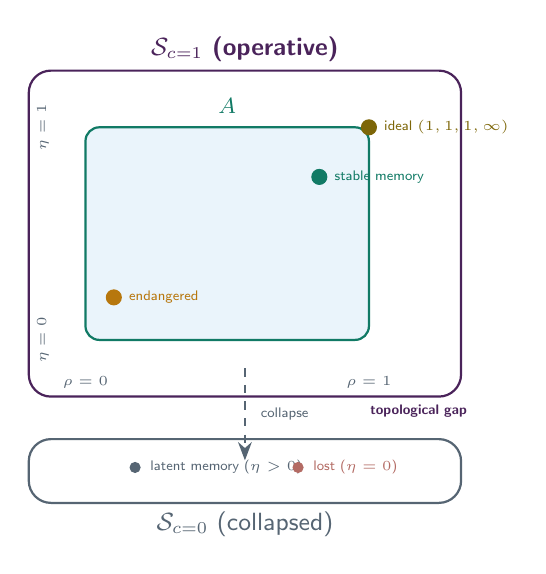
\begin{tikzpicture}[scale=0.9]
  % Component S^+
  \draw[FateViolet,thick,rounded corners=8pt]
    (-0.3,-0.3) rectangle (5.8,4.3);
  \node[font=\sffamily\small\bfseries\color{FateViolet}]
    at (2.75,4.6) {$\fateComp{1}$ (operative)};
  % Admissible region
  \draw[DistTeal,thick,fill=DistLight,rounded corners=5pt]
    (0.5,0.5) rectangle (4.5,3.5);
  \node[font=\sffamily\footnotesize\color{DistTeal}]
    at (2.5,3.8) {$\admRegion$};
  % Axes labels
  \node[font=\tiny\sffamily\color{DistGray}]at(0.5,-0.1){$\survRatio=0$};
  \node[font=\tiny\sffamily\color{DistGray}]at(4.5,-0.1){$\survRatio=1$};
  \node[font=\tiny\sffamily\color{DistGray},rotate=90]
    at(-0.1,0.5){$\repEff=0$};
  \node[font=\tiny\sffamily\color{DistGray},rotate=90]
    at(-0.1,3.5){$\repEff=1$};
  % Ideal corner
  \filldraw[DistGold](4.5,3.5)circle(3pt);
  \node[font=\tiny\sffamily\color{DistGold},right=2pt]
    at(4.5,3.5){ideal $(1,1,1,\mathbf{\infty})$};
  % Endangered point
  \filldraw[DistAmber](0.9,1.1)circle(3pt);
  \node[font=\tiny\sffamily\color{DistAmber},right=2pt]
    at(0.9,1.1){endangered};
  % Stable memory point
  \filldraw[DistTeal](3.8,2.8)circle(3pt);
  \node[font=\tiny\sffamily\color{DistTeal},right=2pt]
    at(3.8,2.8){stable memory};
  % Topological gap arrow
  \draw[-Stealth,dashed,DistGray,thick]
    (2.75,0.1)--(2.75,-1.2)
    node[midway,right=2pt,font=\tiny\sffamily\color{DistGray}]
    {collapse};
  % Component S^0
  \draw[DistGray,thick,rounded corners=8pt]
    (-0.3,-1.8) rectangle (5.8,-0.9);
  \node[font=\sffamily\small\color{DistGray}]
    at(2.75,-2.1){$\fateComp{0}$ (collapsed)};
  \filldraw[DistGray](1.2,-1.3)circle(2pt);
  \node[font=\tiny\sffamily\color{DistGray},right=2pt]
    at(1.2,-1.3){latent memory ($\repEff>0$)};
  \filldraw[DistRed!70](3.5,-1.3)circle(2pt)
    node[right=2pt,font=\tiny\sffamily\color{DistRed!70}]
    {lost ($\repEff=0$)};
  % Gap label
  \node[font=\sffamily\tiny\bfseries\color{FateViolet}]
    at(5.2,-0.5){topological gap};
\end{tikzpicture}
\end{fatediagram}

\section{Fate-Profile Equivalence}

Two distinction pairs have the same fate if and only if their
fate maps agree.

\begin{definition}{Fate-Profile Equivalence}{fate-equiv}
Two distinction pairs $(x,y),(x',y')\in X\times X$ are
\emph{fate-equivalent}, written $(x,y)\approx_\fateMap(x',y')$,
if
\[
  \fateMap(x,y) \;=\; \fateMap(x',y').
\]
\end{definition}

This equivalence relation on $X\times X$ will be used in
Chapter~15 to define fate classes: the equivalence classes
$\fateClasses=(X\times X)/{\approx_\fateMap}$. The reason for
deferring the quotient is conceptual: distinction pairs exist
before their fates. The geometry of $X\times X$ and $\fateSpace$
should be understood before the quotient is formed. Chapter~15
introduces $\fateClasses$ at the moment when population
dynamics require it.

\begin{remark}{What the Fate Map Does Not Record}{fate-limits}
The fate map $\fateMap$ records prospective information about
a distinction pair: survival, repairability, transport reach,
operational status. It does not record:

The \emph{content} of the distinction --- what $x$ and $y$
differ \emph{in} is not captured by $\fateMap(x,y)$.

The \emph{history} of the pair --- how it came to have its
current fate profile is not in $\fateSpace$.

The \emph{mechanism} of collapse or repair --- $\fateMap$
records the outcome, not the process.

These are not defects. They are features: by abstracting away
content, history, and mechanism, the fate map becomes
applicable to distinctions in physics, biology, cognition,
language, and civilization under a single formalism. The
content-, history-, and mechanism-specific theories are special
cases to which the framework applies.
\end{remark}

\begin{chapsummary}
\item The fate space $\fateSpace=[0,1]_\survRatio\times
  [0,1]_\repEff\times\{0,1\}_\collapseInd\times\mathbb{R}_{\ge0}^k$
  records the prospects of a distinction pair under the
  operator family.
\item The four coordinates measure: survival rate, repair
  efficiency, operational status, and transport reach.
\item $\fateSpace$ has two connected components $\fateComp{1}$
  (operative) and $\fateComp{0}$ (collapsed), separated by
  the discrete topology of $\collapseInd$.
\item The Collapse Discontinuity Meta-Theorem: no continuous
  path connects $\fateComp{1}$ to $\fateComp{0}$; collapse
  is topologically irreversible.
\item The fate map $\fateMap:X\times X\to\fateSpace$ is the
  primary object of Part~III; everything in Parts~IV--VI is
  derived from it.
\item Fate-profile equivalence $\approx_\fateMap$ partitions
  $X\times X$ into fate classes, introduced formally in
  Chapter~15.
\end{chapsummary}

% ============================================================
%  (Skip chapters 11–14 — already written)
%  (Skip chapters 13A, 13B — already written)
%  (Skip chapters 15A–15D — already written)
% ============================================================


% ============================================================
%  CHAPTER 15 — FATE CLASSES AND POPULATION DYNAMICS
% ============================================================



% ============================================================
%  CHAPTER 11 — FATE METRICS AND CONTINUITY
% ============================================================

\chapter{Fate Metrics and Continuity}
\label{ch:fate-metrics}

\begin{epigraph}{Two points may be close together without their
  futures being close together.}{Observation underlying this chapter}
\end{epigraph}

\begin{objectives}
\item Define fate distance as a family of metrics on the connected
  components of fate space.
\item Establish local continuity of the fate map under admissible
  operator families.
\item Introduce fate sensitivity as the local Lipschitz constant of
  the fate map.
\item Show that the singular set is precisely the locus of infinite
  fate sensitivity, suturing this chapter to Chapter~12.
\end{objectives}

The previous chapter introduced fate space
\[
  \fateSpace
  \;=\;
  [0,1]_{\survRatio}
  \times
  [0,1]_{\repEff}
  \times
  \{0,1\}_{\collapseInd}
  \times
  \mathbb{R}_{\ge0}^{k}
\]
and the fate map
\[
  \fateMap:\distPairs\longrightarrow\fateSpace.
\]
The existence of a fate map allows distinction pairs to be
compared not merely by their present observational separation
but by the trajectories available to that separation under
transformation. Distinctions that appear similar at a single
instant may possess radically different futures. The purpose
of fate geometry is therefore not to describe what distinctions
are, but what may become of them.

To reason about such questions we require a notion of distance
on fate space, and a corresponding notion of continuity for the
fate map. The topological structure of $\fateSpace$, however,
is not uniform: the discrete collapse coordinate
$\collapseInd\in\{0,1\}$ partitions $\fateSpace$ into two
connected components. Fate distance and fate continuity are
therefore defined component-wise.

\section{Fate Distance}

\begin{definition}{Connected Components of Fate Space}%
  {fate-components}
The space $\fateSpace$ has exactly two connected components,
\[
  \fateComp{1}
  \;=\;
  [0,1]_{\survRatio}\times[0,1]_{\repEff}
    \times\{1\}\times\mathbb{R}_{\ge0}^{k},
\]
\[
  \fateComp{0}
  \;=\;
  [0,1]_{\survRatio}\times[0,1]_{\repEff}
    \times\{0\}\times\mathbb{R}_{\ge0}^{k}.
\]
A fate profile $s\in\fateSpace$ belongs to $\fateComp{1}$ if
$\collapseInd(s)=1$ (the distinction is operationally present)
and to $\fateComp{0}$ if $\collapseInd(s)=0$ (it has collapsed).
\end{definition}

\begin{definition}{Fate Distance}{fate-distance}
Let $s=(\survRatio,\repEff,\collapseInd,\boldsymbol{\tau})$ and
$s'=(\survRatio',\repEff',\collapseInd',\boldsymbol{\tau}')$ be
fate profiles belonging to the same connected component of
$\fateSpace$.
The \emph{fate distance} is
\[
  \fateDist{s}{s'}
  \;=\;
  |\survRatio-\survRatio'|
  \;+\;
  |\repEff-\repEff'|
  \;+\;
  \|\boldsymbol{\tau}-\boldsymbol{\tau}'\|_{1}.
\]
The collapse coordinate $\collapseInd$ is omitted because it is
constant within each component and cannot contribute to
intra-component distance.

For profiles in \emph{different} components, fate distance is
undefined. The topological gap between components is addressed
by the Collapse Discontinuity Theorem
(\cref{meta:collapse-disc}) and is the subject of
Chapter~12.
\end{definition}

\begin{proposition}{Fate Distance is a Metric on Each Component}%
  {fate-metric}
On each connected component $\fateComp{c}$, the fate distance
$d_{\fateSpace}$ is a metric.
\begin{proof}
Within $\fateComp{c}$ the collapse coordinate is the constant
$c\in\{0,1\}$ and contributes nothing to the distance formula.
The remaining coordinates are $\survRatio,\repEff\in[0,1]$ and
$\boldsymbol{\tau}\in\mathbb{R}_{\ge0}^k$.

\emph{Positivity.} Each term $|\survRatio-\survRatio'|$,
$|\repEff-\repEff'|$, $\|\boldsymbol{\tau}-\boldsymbol{\tau}'\|_1$
is non-negative. Their sum is zero iff each term is zero, which
holds iff $\survRatio=\survRatio'$, $\repEff=\repEff'$, and
$\boldsymbol{\tau}=\boldsymbol{\tau}'$, i.e., iff $s=s'$.

\emph{Symmetry.} $|a-b|=|b-a|$ and $\|\mathbf{u}-\mathbf{v}\|_1
=\|\mathbf{v}-\mathbf{u}\|_1$ for all real values.

\emph{Triangle inequality.} For any third profile
$s''=(\survRatio'',\repEff'',c,\boldsymbol{\tau}'')$,
\begin{align*}
  \fateDist{s}{s''}
  &= |\survRatio-\survRatio''|
     +|\repEff-\repEff''|
     +\|\boldsymbol{\tau}-\boldsymbol{\tau}''\|_1 \\
  &\le
    (|\survRatio-\survRatio'|+|\survRatio'-\survRatio''|)
    +(|\repEff-\repEff'|+|\repEff'-\repEff''|) \\
  &\quad
    +(\|\boldsymbol{\tau}-\boldsymbol{\tau}'\|_1
     +\|\boldsymbol{\tau}'-\boldsymbol{\tau}''\|_1) \\
  &= \fateDist{s}{s'} + \fateDist{s'}{s''}.
\end{align*}
Hence $d_{\fateSpace}$ satisfies all metric axioms on $\fateComp{c}$.
\end{proof}
\end{proposition}

\begin{remark}{Fate Distance is Not Observational Distance}%
  {fate-vs-obs}
The fate distance $d_{\fateSpace}$ and the observational
pseudometric $\distMetric$ measure orthogonal properties.
Two distinction pairs may be observationally close
($\distDist{p}{q}$ small) while their fate profiles are distant
($\fateDist{\fateMap(p)}{\fateMap(q)}$ large), and vice versa.
A pair of states nearly indistinguishable today may face
entirely different futures. Conversely, two currently well-separated
pairs may share identical fates under the same operator family.
Fate geometry therefore captures information that observational
geometry cannot.
\end{remark}

\section{Continuity of the Fate Map}

\begin{definition}{Fate Continuity}{fate-continuity-defn}
The fate map $\fateMap$ is \emph{continuous at} $(x,y)\in\distPairs$
if $\fateMap(x,y)$ and all sufficiently nearby pairs share the
same connected component of $\fateSpace$, and for every
$\varepsilon>0$ there exists $\delta>0$ such that
\[
  \distDist{(x,y)}{(x',y')} < \delta
  \;\Longrightarrow\;
  \fateDist{\fateMap(x,y)}{\fateMap(x',y')} < \varepsilon.
\]
The fate map is \emph{continuous} if it is continuous at every
point of $\distPairs$.
\end{definition}

The condition that nearby pairs share the same connected component
is not redundant: pairs near a collapse event may lie in different
components, and the distance formula is undefined across components.
Continuity requires that collapse events are isolated, not merely
that the real-valued coordinates vary continuously.

\begin{theorem}{Local Continuity of the Fate Map}{local-cont}
Let $\transfam$ be an admissible transformation family such that
the survival ratio $\survRatio_\transfam(x,y)$ and repair
efficiency $\repEff(x,y)$ vary continuously with respect to
$\distMetric$, and the transport coordinates
$\boldsymbol{\tau}(x,y)$ are constructed from continuous operator
actions on $\distPairs$. Then $\fateMap$ is continuous on the
interior of each non-collapse region
\[
  \distPairs^{+}
  \;=\;
  \{(x,y)\in\distPairs : \collapseInd(x,y)=1\}.
\]
\begin{proof}
Fix $(x,y)\in\distPairs^{+}$, so $\collapseInd(x,y)=1$.
By assumption, $\survRatio_\transfam$ and $\repEff$ are continuous
at $(x,y)$. Since $\distPairs^{+}$ is open in $\distPairs$ (it
is the preimage of the open set $\{c=1\}$ in the Sierpi\'{n}ski
topology on $\{0,1\}$), there exists a neighbourhood of $(x,y)$
contained in $\distPairs^{+}$. Within this neighbourhood all
pairs share the component $\fateComp{1}$, so fate distance is
defined.

Given $\varepsilon>0$, continuity of $\survRatio_\transfam$
provides $\delta_1$ such that
$|\survRatio_\transfam(x,y)-\survRatio_\transfam(x',y')|
<\varepsilon/3$
whenever $\distDist{(x,y)}{(x',y')}<\delta_1$.
Continuity of $\repEff$ provides $\delta_2$ analogously.
Continuity of each transport coordinate provides $\delta_3$.
Setting $\delta=\min(\delta_1,\delta_2,\delta_3)$ gives
\[
  \fateDist{\fateMap(x,y)}{\fateMap(x',y')}
  \;<\;
  \tfrac{\varepsilon}{3}+\tfrac{\varepsilon}{3}
  +\tfrac{\varepsilon}{3}
  \;=\;\varepsilon
\]
for all $(x',y')$ with $\distDist{(x,y)}{(x',y')}<\delta$.
\end{proof}
\end{theorem}

\begin{remark}{The Assumption is on Operators, Not on State Space}%
  {cont-assumption}
The continuity hypotheses of \cref{thm:local-cont} are conditions
on the operator family $\transfam$, not on the underlying state
space $X$. They are satisfied, for example, whenever $X$ is a
normed space and the survival and repair operators are given by
Lipschitz maps. The theorem therefore applies to all standard
physical and computational models of transformation, while leaving
open the possibility of discontinuous operators --- which are
precisely the objects of Chapter~12.
\end{remark}

\section{Fate Sensitivity and Lipschitz Regularity}

Continuity guarantees that nearby distinctions have nearby futures.
A quantitative strengthening asks at what \emph{rate} futures can
diverge as pairs are perturbed.

\begin{definition}{Fate Sensitivity}{fate-sens-defn}
The \emph{fate sensitivity} of $\fateMap$ at $(x,y)\in\distPairs$
is
\[
  \fateSens{x,y}
  \;=\;
  \limsup_{(x',y')\to(x,y)}
  \frac{
    \fateDist{\fateMap(x,y)}{\fateMap(x',y')}
  }{
    \distDist{(x,y)}{(x',y')}
  }.
\]
This is the local Lipschitz constant of $\fateMap$ at $(x,y)$.
\end{definition}

\begin{definition}{Lipschitz Fate Map}{lipschitz-fate}
The fate map is \emph{Lipschitz} if there exists a global constant
$\fateLip>0$ such that
\[
  \fateDist{\fateMap(p)}{\fateMap(q)}
  \;\le\;
  \fateLip\cdot\distDist{p}{q}
\]
for all $p,q$ in the same non-collapse region of $\distPairs$.
Equivalently, $\sup_{p\in\distPairs^+}\fateSens{p}\le\fateLip<\infty$.
\end{definition}

The Lipschitz constant $\fateLip$ quantifies the fragility of
fate: small Lipschitz constants indicate that futures are robust
to perturbation; large constants indicate that small changes in
the distinction pair produce large changes in fate. For specific
operator families, $\fateLip$ can be computed from the operator
norms of the survival and repair maps.

\begin{proposition}{Linear Observation Bound}{linear-lip}
Let $X=\mathbb{R}^n$ with the Euclidean norm,
$\obs=\{o_j:X\to\mathbb{R}\}_{j=1}^m$ a finite family of
linear observation maps, and suppose the survival and repair
operators are given by matrices $S,R\in\mathbb{R}^{n\times n}$.
Then the fate map is Lipschitz with constant
\[
  \fateLip
  \;\le\;
  \max_{j}\bigl(\|S\|_{\mathrm{op}}+\|R\|_{\mathrm{op}}\bigr)
  \cdot
  \max_{j}\|o_j\|_{\mathrm{op}}.
\]
\begin{proof}
The survival ratio coordinate satisfies
$|\survRatio(p)-\survRatio(q)|
\le\|S\|_{\mathrm{op}}\cdot\distDist{p}{q}$
by linearity and the definition of the operator norm.
The repair efficiency coordinate satisfies
$|\repEff(p)-\repEff(q)|
\le\|R\|_{\mathrm{op}}\cdot\distDist{p}{q}$
by the same argument.
Summing gives the stated bound.
\end{proof}
\end{proposition}

The key structural theorem suturing this chapter to Chapter~12
is the following, which shows that fate sensitivity is not merely
a quantitative measure but a geometric one: its singularities
are exactly the points where Chapter~12's analysis begins.

\begin{theorem}{Singular Set as Infinite Sensitivity}%
  {sing-is-infinite}
The singular set $\singSet$ of the fate map coincides with the
locus of infinite fate sensitivity:
\[
  \singSet
  \;=\;
  \bigl\{(x,y)\in\distPairs : \fateSens{x,y}=+\infty\bigr\}.
\]
\begin{proof}
$(\supseteq)$: Suppose $\fateSens{x,y}=+\infty$. Then for
every $M>0$ and every $\delta>0$, there exists $(x',y')$ with
$\distDist{(x,y)}{(x',y')}<\delta$ yet
$\fateDist{\fateMap(x,y)}{\fateMap(x',y')}>M\cdot\delta$.
No such behaviour is compatible with continuity at $(x,y)$.
Hence $\fateMap$ is discontinuous at $(x,y)$, so
$(x,y)\in\singSet$.

$(\subseteq)$: Suppose $\fateSens{x,y}<\infty$. Then $\fateMap$
is locally Lipschitz at $(x,y)$, hence continuous there. Thus
$(x,y)\notin\singSet$.
\end{proof}
\end{theorem}

\section{Fate Criticality}

The Singular Set as Infinite Sensitivity theorem establishes
that $\fateSens{x,y}=+\infty$ characterizes exactly the points
of $\singSet$. A natural question follows: can infinite
sensitivity be detected in advance, before a distinction pair
reaches the singular set? The following theorem provides a
positive answer.

\begin{theorem}{Fate Criticality Theorem}{fate-criticality}
Let $\gamma:[0,1]\to\distPairs$ be a continuous path with
$\gamma(0)=(x,y)$ and $\lim_{t\to 1}\gamma(t)\in\singSet$.
Then
\[
  \fateSens{\gamma(t)}\;\longrightarrow\;+\infty
  \qquad\text{as }t\to 1.
\]
That is: as a distinction pair approaches a singular stratum,
its fate sensitivity diverges.
\begin{proof}
Suppose for contradiction that $\fateSens{\gamma(t)}$ remains
bounded along the path: $\fateSens{\gamma(t)}\le M<\infty$ for
all $t\in[0,1)$. Then $\fateMap\circ\gamma$ is locally Lipschitz
with constant $M$ along $\gamma$, hence continuous on $[0,1)$.

Since $\gamma$ is continuous and $\distPairs$ is a metric space,
$\gamma(t)$ converges to a point $p^*\in\singSet$ as $t\to 1$.
By the Singular Set as Infinite Sensitivity theorem
(\cref{thm:sing-is-infinite}), $\fateSens{p^*}=+\infty$.
But if $\fateMap$ were locally Lipschitz at $p^*$ with
constant $M$, it would be continuous there, contradicting
$p^*\in\singSet$. Hence the assumption fails: $\fateSens{\gamma(t)}$
must diverge as $t\to 1$.
\end{proof}
\end{theorem}

\begin{remark}{Predictive Interpretation}{criticality-predict}
The Fate Criticality Theorem gives a predictive criterion for
impending fate singularities. A distinction pair approaching
collapse, forgetting, or repair-threshold will exhibit
increasing fate sensitivity before the singularity is reached.
Monitoring $\fateSens{x,y}$ therefore provides advance warning
of qualitative fate transitions.

This has concrete interpretations at every scale. In physical
systems, rising sensitivity near a phase transition corresponds
to critical slowing down and diverging susceptibility. In
cognitive systems, rising sensitivity near a forgetting
threshold corresponds to increased vulnerability of a memory
to interference. In social systems, rising sensitivity near
an institutional stratum corresponds to the brittleness
characteristic of organizations approaching failure. In each
case the same mathematical object --- fate sensitivity ---
provides the observable signature.
\end{remark}

\begin{chapsummary}
\item Fate space $\fateSpace$ has two connected components
  $\fateComp{1}$ and $\fateComp{0}$ separated by the discrete
  collapse coordinate.
\item Fate distance $d_{\fateSpace}$ is a metric on each component,
  omitting the collapse coordinate as constant within a component.
\item The fate map is continuous on the interior of each
  non-collapse region whenever the operator family acts
  continuously on distinction pairs.
\item Fate sensitivity $\sigma_{\fateMap}$ is the local Lipschitz
  constant; its divergence to infinity is equivalent to
  discontinuity of the fate map.
\item The singular set $\singSet$ is the locus of infinite
  sensitivity. Its structure is the subject of Chapter~12.
\item The Fate Criticality Theorem: as a distinction pair
  approaches any singular stratum, its fate sensitivity
  diverges. This provides a predictive signature of impending
  fate transitions.
\end{chapsummary}

% ============================================================
%  CHAPTER 12 — FATE SINGULARITIES AND BIFURCATIONS
% ============================================================

\chapter{Fate Singularities and Bifurcations}
\label{ch:fate-sing}

\begin{epigraph}{The singular points are not defects of the
  theory. They are the theory's most important predictions.}%
  {Paraphrase of Ren\'e Thom}
\end{epigraph}

\begin{objectives}
\item Identify the singular set $\singSet$ as the union of four
  qualitatively distinct strata.
\item Prove that collapse events are topological singularities,
  not merely large quantitative changes.
\item Characterize repair threshold, transport horizon, and
  forgetting singularities as bifurcations in fate space.
\item Establish that the strata are generically smooth
  submanifolds away from their mutual intersections.
\item Show that historical events --- scientific revolutions,
  institutional collapse, paradigm shifts --- are crossings of
  specific strata.
\end{objectives}

The previous chapter established that the fate map is
continuous on the interior of each non-collapse region, and
that the singular set $\singSet$ is precisely the locus of
infinite fate sensitivity. This chapter characterizes the
geometry of $\singSet$.

The singular set is not homogeneous. Different points of
$\singSet$ correspond to qualitatively different modes of fate
transition, arising from different coordinates of the fate map.
The natural decomposition of $\singSet$ into strata makes this
taxonomy precise.

\section{The Singular Set and Its Strata}

Recall from Chapter~11 that
\[
  \singSet
  \;=\;
  \bigl\{(x,y)\in\distPairs
  : \fateMap\text{ is discontinuous at }(x,y)\bigr\}.
\]

\begin{definition}{Fate Strata}{fate-strata}
The singular set decomposes as
\[
  \singSet
  \;=\;
  \strataC\;\cup\;\strataR\;\cup\;\strataT\;\cup\;\strataF,
\]
where each stratum is defined by the coordinate of $\fateSpace$
responsible for the discontinuity:
\begin{itemize}[nosep,leftmargin=2em]
  \item $\strataC$ (\emph{collapse stratum}): locus where
    $\collapseInd$ changes discontinuously from~$1$ to~$0$.
  \item $\strataR$ (\emph{repair stratum}): locus where $\repEff$
    jumps discontinuously, marking the appearance or disappearance
    of a repair pathway.
  \item $\strataT$ (\emph{transport stratum}): locus where a
    transport coordinate $\tau_i$ changes discontinuously, marking
    a reachability horizon.
  \item $\strataF$ (\emph{forgetting stratum}): locus where
    $\survRatio$ drops discontinuously to zero, marking the onset
    of irreversible forgetting.
\end{itemize}
\end{definition}

The strata are not mutually exclusive at their boundaries: a
point may lie in multiple strata simultaneously, corresponding
to a fate event involving more than one coordinate. Such
intersections are the most structurally complex points of
$\singSet$ and are discussed in
\cref{sec:stratum-intersections}.

\section{Collapse Singularities}

The collapse stratum $\strataC$ is the most dramatic. The
collapse coordinate $\collapseInd$ is discrete: it cannot vary
continuously. Any change in its value is therefore a
topological discontinuity.

\begin{theorem}{Collapse Events are Topological Singularities}%
  {collapse-topo}
Every point of $\strataC$ is a topological singularity of the
fate map: the fate map cannot be extended continuously across
$\strataC$.
\begin{proof}
Let $(x,y)\in\strataC$. By definition, $\collapseInd(x,y)=1$
yet every neighbourhood of $(x,y)$ in $\distPairs$ contains
points $(x',y')$ with $\collapseInd(x',y')=0$.

The space $\fateSpace$ is equipped with the product topology.
The factor $\{0,1\}$ carries the discrete topology, in which
$\{0\}$ and $\{1\}$ are both open and closed. The preimage
$\fateMap^{-1}(\{c=1\})$ and $\fateMap^{-1}(\{c=0\})$ are
therefore required to be open sets if $\fateMap$ is continuous.
But their union is all of $\distPairs$ and they are disjoint,
so continuity of $\collapseInd\circ\fateMap$ requires
$\distPairs$ to be disconnected in a neighbourhood of $(x,y)$.

Since by hypothesis every neighbourhood of $(x,y)$ contains
points of both $\distPairs^+$ and $\distPairs^0$, no such
disconnected neighbourhood exists. Therefore $\fateMap$ is
discontinuous at $(x,y)$, and the discontinuity cannot be
removed by any continuous extension.
\end{proof}
\end{theorem}

\begin{remark}{Collapse is not Degradation}{collapse-not-degrad}
This theorem provides the formal distinction between
\emph{degradation} and \emph{collapse}. Degradation corresponds
to movement within $\fateComp{1}$: the survival ratio $\survRatio$
decreases, the repair efficiency $\repEff$ may decline, but the
distinction remains operationally present. Collapse corresponds
to crossing $\strataC$ into $\fateComp{0}$: the distinction
ceases to be operationally present. The two processes differ not
in degree but in kind. A degrading distinction can in principle
be repaired; a collapsed distinction cannot be repaired from
within the same operator family that caused the collapse,
because it no longer exists as an object in $\distPairs^+$.
\end{remark}

\begin{corollary}{Scientific Revolutions as Collapse Events}%
  {revolutions-collapse}
A scientific revolution in the sense of Kuhn, in which a
previously operative distinction ceases to organize empirical
inquiry, is a crossing of $\strataC$. It is therefore not a
large quantitative change in theory but a topological
singularity: no continuous deformation of the prior framework
produces it.
\end{corollary}

\section{Repair Threshold Singularities}

The repair stratum $\strataR$ marks a qualitatively different
event: the sudden appearance or disappearance of a repair
pathway.

\begin{definition}{Repair Threshold}{repair-threshold}
A distinction pair $(x,y)$ lies on the repair stratum $\strataR$
if the repair efficiency $\repEff(x,y)$ is discontinuous at
$(x,y)$: specifically, if
\[
  \liminf_{(x',y')\to(x,y)}\repEff(x',y')
  \;\neq\;
  \limsup_{(x',y')\to(x,y)}\repEff(x',y').
\]
\end{definition}

Repair threshold singularities correspond to the appearance of
memory. When $\repEff$ jumps from~$0$ to a positive value, a
distinction that was previously irrecoverable after damage
suddenly becomes recoverable. This is the formal analogue of
the appearance of an error-correcting code, a biological repair
mechanism, or an archival system.

\begin{proposition}{Repair Thresholds are Bifurcations}%
  {repair-bifurc}
At a repair threshold singularity, the qualitative structure of
the fate map changes: the fate of a distinction pair transitions
from the regime of permanent loss to the regime of managed
degradation.
\begin{proof}
Below threshold ($\repEff=0$), damage to the distinction is
permanent: the repair efficiency coordinate of $\fateMap$
contributes nothing to $\fateDist{\fateMap(p)}{\fateMap(q)}$
and the distinction evolves under pure degradation dynamics.
Above threshold ($\repEff>0$), damage is recoverable and the
evolution is governed by the repair--degradation balance.
These are qualitatively distinct dynamical regimes. The jump
in $\repEff$ at the threshold constitutes a bifurcation in the
fate map.
\end{proof}
\end{proposition}

\section{Transport Horizon Singularities}

The transport stratum $\strataT$ arises from the finite extent
of distinguishability transport.

\begin{definition}{Transport Horizon}{transport-horizon}
A distinction pair $(x,y)$ lies on the transport stratum
$\strataT$ if at least one transport coordinate $\tau_i(x,y)$
is discontinuous at $(x,y)$: specifically, if
$(x,y)$ lies on the boundary of a reachability domain for the
relevant transport operator.
\end{definition}

Transport horizon singularities separate distinction pairs that
can be communicated, synchronized, or propagated from those
that cannot. Inside the reachability domain, transport is
available and the transport coordinate $\tau_i$ is finite.
Outside, transport is unavailable and $\tau_i=+\infty$.

The boundary between these regions is $\strataT$.

\section{Forgetting Singularities}

The forgetting stratum $\strataF$ marks the onset of
irreversible forgetting.

\begin{definition}{Forgetting Stratum}{forgetting-strat}
A distinction pair $(x,y)$ lies on the forgetting stratum
$\strataF$ if the survival ratio $\survRatio_\transfam(x,y)$
drops discontinuously to zero:
\[
  \survRatio_\transfam(x,y)=0
  \quad\text{and}\quad
  \limsup_{(x',y')\to(x,y)}\survRatio_\transfam(x',y')>0.
\]
\end{definition}

Unlike collapse, forgetting need not destroy the distinction
immediately: $\collapseInd$ may remain~$1$ while $\survRatio$
drops to zero. The distinction is present but no longer
survives transformation. The semantic horizon of
\EOD{Definition~5.3} is the state-space image of~$\strataF$.

\section{Stratification of the Singular Set}
\label{sec:stratum-intersections}

\begin{theorem}{Generic Smoothness of Strata}%
  {generic-smooth}
For a generic admissible operator family $\transfam$, each
stratum $\strataC$, $\strataR$, $\strataT$, $\strataF$ is a
smooth submanifold of $\distPairs$ of codimension~$1$, away
from the intersections of distinct strata.
\begin{proof}
Each stratum is defined as the zero set (or jump set) of a
smooth function on $\distPairs$. Specifically: the collapse
stratum arises from the indicator function
$\collapseInd\circ\fateMap:\distPairs\to\{0,1\}$ and is the
boundary between its preimages; the repair stratum is the zero
set of $\repEff\circ\fateMap$; the transport stratum is the
boundary of a reachability domain; the forgetting stratum is
the zero set of $\survRatio_\transfam\circ\fateMap$.

For a generic operator family, these functions are regular at
their zero sets: their gradients are nonzero. By the regular
level set theorem, each zero set is a smooth submanifold of
codimension~$1$.

At intersections $\strataC\cap\strataR$, $\strataC\cap\strataT$,
etc., two or more defining functions simultaneously vanish.
Generically these intersections are smooth submanifolds of
higher codimension, and together the strata form a
Whitney-regular stratified space. The full strata themselves
(away from intersections) are smooth manifolds of
codimension~$1$.
\end{proof}
\end{theorem}

\begin{remark}{Strata as Historical Event Surfaces}%
  {strata-history}
The smooth strata of $\singSet$ are the surfaces in
$\distPairs$ at which qualitative change occurs. A system
moving through $\distPairs$ under the action of operators spends
most of its existence in the regular interior, where fate
varies continuously. The occasional crossing of a stratum is
the formal image of an event: a memory forms, a capability is
lost, a paradigm shifts, a civilization crosses a threshold.
The stratification of $\singSet$ provides a taxonomy of such
events organized by which coordinate of fate space undergoes
the discontinuity.
\end{remark}

\begin{fatediagram}{Summary of Singular Strata}
\centering
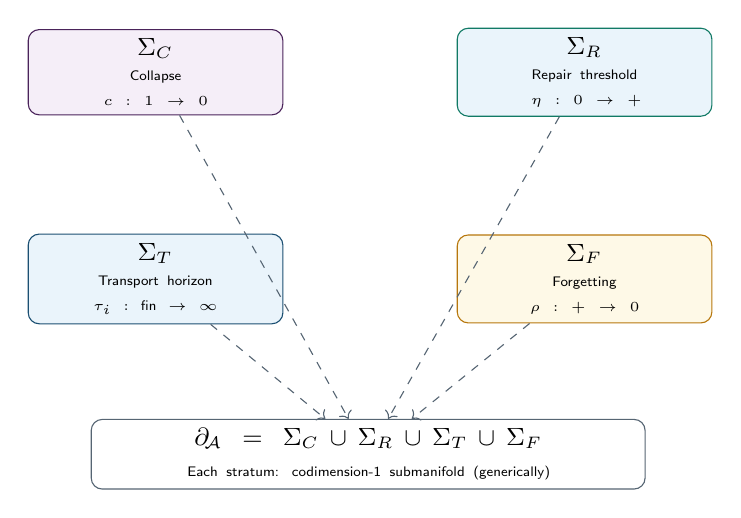
\begin{tikzpicture}[node distance=2.2cm]
  \node[draw=FateViolet,fill=FateLilac,rounded corners,
    text width=3cm,align=center,font=\small\sffamily]
    (SC) {$\strataC$\\[-2pt]{\tiny Collapse}\\[-2pt]
    {\tiny $c:1\to0$}};
  \node[draw=DistTeal,fill=DistLight,rounded corners,
    text width=3cm,align=center,font=\small\sffamily,
    right=of SC]
    (SR) {$\strataR$\\[-2pt]{\tiny Repair threshold}\\[-2pt]
    {\tiny $\repEff:0\to{+}$}};
  \node[draw=DistBlue,fill=DistLight,rounded corners,
    text width=3cm,align=center,font=\small\sffamily,
    below=1.5cm of SC]
    (ST) {$\strataT$\\[-2pt]{\tiny Transport horizon}\\[-2pt]
    {\tiny $\tau_i:\text{fin}\to\infty$}};
  \node[draw=DistAmber,fill=DistGoldBg,rounded corners,
    text width=3cm,align=center,font=\small\sffamily,
    right=of ST]
    (SF) {$\strataF$\\[-2pt]{\tiny Forgetting}\\[-2pt]
    {\tiny $\survRatio:+\to0$}};
  \node[draw=DistGray,fill=white,rounded corners,
    text width=6.8cm,align=center,font=\small\sffamily,
    below=1.2cm of ST,xshift=2.7cm]
    (SG) {$\singSet=\strataC\cup\strataR
      \cup\strataT\cup\strataF$\\
    {\tiny Each stratum: codimension-1 submanifold (generically)}};
  \draw[->,DistGray,dashed](SC)--(SG);
  \draw[->,DistGray,dashed](SR)--(SG);
  \draw[->,DistGray,dashed](ST)--(SG);
  \draw[->,DistGray,dashed](SF)--(SG);
\end{tikzpicture}
\end{fatediagram}

\begin{chapsummary}
\item The singular set $\singSet$ decomposes into four strata:
  collapse $\strataC$, repair threshold $\strataR$, transport
  horizon $\strataT$, forgetting $\strataF$.
\item Collapse events are topological singularities: no
  continuous path in $\fateSpace$ crosses $\strataC$.
\item Repair threshold singularities are bifurcations: the
  qualitative fate regime changes from permanent loss to managed
  degradation.
\item Transport and forgetting singularities mark the boundaries
  of reachability and survival.
\item Generically, each stratum is a smooth codimension-$1$
  submanifold; their intersections form a Whitney-regular
  stratified space.
\item Historical events --- revolutions, collapses, paradigm
  shifts --- are crossings of specific strata.
\end{chapsummary}

% ============================================================
%  CHAPTER 13 — ADMISSIBILITY AS FATE SELECTION
% ============================================================

\chapter{Admissibility as Fate Selection}
\label{ch:admissibility-fate}

\begin{epigraph}{The question is not which states are allowed.
  The question is which futures are allowed.}%
  {The central reorientation of this chapter}
\end{epigraph}

\begin{objectives}
\item Reinterpret admissibility as a constraint on fates rather
  than on states.
\item Define the admissibility operator as a restriction of
  $\distPairs$ to pairs with admissible fate profiles.
\item Prove the Admissibility Pullback Theorem: every
  admissibility manifold in state space is the pullback of an
  admissible fate region under $\fateMap$.
\item Show that admissibility geometry in the outer volumes is a
  special case of fate geometry developed here.
\end{objectives}

Previous treatments of admissibility, including the extensive
development in \EOD{Chapters~14--15}, described admissibility
as a restriction on possible continuations of a system.
A state or trajectory is admissible if following it preserves
the volume of future possibility. The admissibility manifold
$\adm(x,t)$ encodes which states lie within the admissible
region at each time.

The fate-theoretic framework provides a deeper interpretation~\cite{amari2016}.
Admissibility is not selection on states. It is selection on
fates. The admissibility manifold is not a primitive geometric
object but a derived one: it is the preimage of an admissible
region in fate space under the fate map.

\section{Admissible Fate Regions}

\begin{definition}{Admissible Fate Region}{adm-fate-region}
An \emph{admissible fate region} is a subset
$\admRegion\subseteq\fateSpace$ specifying the fate profiles
deemed acceptable. A distinction pair $(x,y)\in\distPairs$
is \emph{admissible} if
\[
  \fateMap(x,y)\in\admRegion.
\]
\end{definition}

The definition relocates the locus of admissibility from state
space to fate space. This is not a terminological shift: it
changes what must be specified. Under the classical approach,
admissibility requires specifying a manifold $\adm(x,t)$ in
state space for each time $t$. Under the fate-theoretic
approach, admissibility requires specifying a region $\admRegion$
in the fixed space $\fateSpace$, and the time-dependent state-space
geometry follows by pullback.

\section{The Admissibility Operator}

\begin{definition}{Admissibility Operator}{adm-op-defn}
The \emph{admissibility operator} is the restriction
\[
  \admOp:\distPairs\;\longrightarrow\;\distPairs,
  \qquad
  \admOp(\distPairs)
  \;=\;
  \bigl\{(x,y)\in\distPairs
    : \fateMap(x,y)\in\admRegion\bigr\}.
\]
Equivalently, $\admOp = \fateMap^{-1}(\admRegion)$ viewed as a
subspace of $\distPairs$.
\end{definition}

\begin{remark}{Restriction, Not Partial Function}%
  {adm-not-partial}
The admissibility operator is defined as a \emph{restriction}
of $\distPairs$, not as a map sending inadmissible pairs to
$\varnothing$. This avoids the difficulties of partial functions
and aligns with the standard pullback construction: the
admissible pairs form a subspace, and the complement of that
subspace is simply not in the domain of the restricted operator.
Dynamical evolution under admissible operators then consists in
trajectories that remain within $\admOp(\distPairs)$ at each
step.
\end{remark}

\begin{proposition}{Admissibility Operator as Pullback}%
  {adm-pullback-prop}
The admissibility operator satisfies
\[
  \admOp(\distPairs)
  \;=\;
  \fateMap^{-1}(\admRegion).
\]
If $\admRegion$ is open (respectively closed) in $\fateSpace$,
then $\admOp(\distPairs)$ is open (respectively closed) in
$\distPairs$.
\begin{proof}
The first statement is the definition rewritten. The
topological statement follows because $\fateMap$ is continuous
on $\distPairs^+$ (\cref{thm:local-cont}) and the preimage of
an open set under a continuous map is open; dually for closed sets.
\end{proof}
\end{proposition}

\section{The Admissibility Pullback Theorem}

The central result of this chapter shows that the admissibility
manifolds appearing throughout \textit{The Ecology of
Distinctions} --- the geometric objects
$\adm(x,t)$ whose volume $\Vol(\adm(t))$ is the primary
conserved quantity of that framework --- are not primitive
constructions. They are pullbacks of fate-space regions under
the fate map.

\begin{metatheorem}{Admissibility Pullback Theorem}%
  {adm-pullback}
Every admissibility manifold in state space is the pullback of
an admissible fate region in $\fateSpace$ under the fate map.
Specifically, for any admissible region $\admRegion\subseteq\fateSpace$,
the corresponding admissibility manifold in $\distPairs$ is
\[
  \adm_{\distPairs}
  \;=\;
  \fateMap^{-1}(\admRegion)
  \;=\;
  \bigl\{(x,y)\in\distPairs
    : \fateMap(x,y)\in\admRegion\bigr\}.
\]
Conversely, every admissibility manifold in the sense of
\EOD{Chapter~14} arises in this way for some choice of
admissible fate region $\admRegion\subseteq\fateSpace$.
\begin{proof}
\emph{Forward direction.} Given $\admRegion\subseteq\fateSpace$,
the set $\fateMap^{-1}(\admRegion)$ is a subset of $\distPairs$
consisting precisely of those distinction pairs whose fate
profile lies in $\admRegion$. By
\cref{prop:adm-pullback-prop}, this set is open or closed in
$\distPairs$ according to the topology of $\admRegion$.
It therefore constitutes an admissibility manifold in the
distinction-pair space.

\emph{Converse direction.} Let $\mathcal{M}\subseteq\distPairs$
be any admissibility manifold in the sense of \EOD{Chapter~14}:
a set of distinction pairs satisfying some admissibility
criterion expressed in terms of future reachability volume.
Define $\admRegion = \fateMap(\mathcal{M})\subseteq\fateSpace$.
Then $\mathcal{M}\subseteq\fateMap^{-1}(\admRegion)$.
For the reverse inclusion, note that any pair with fate profile
in $\fateMap(\mathcal{M})$ has a fate profile achievable by
some admissible pair, hence itself satisfies the admissibility
criterion. Thus $\mathcal{M}=\fateMap^{-1}(\admRegion)$.
\end{proof}
\end{metatheorem}

\begin{trilogylink}{Admissibility Geometry in the Outer Volumes}
In \textit{Persistence Before Truth}, admissibility appears as
a constraint on reconstruction operators: only admissible
reconstructions are available to restore a distinction.

In \textit{The Ecology of Distinctions}, admissibility becomes
a geometric manifold $\adm(x,t)$ in state space whose volume
$\Vol(\adm(t))$ measures future possibility. The Generative
Admissibility Principle (\EOD{Chapter~15}) identifies
$\Vol(\adm(t))$ as the primary conserved quantity.

The Admissibility Pullback Theorem shows that both of these are
the same object viewed through different projections of the
same fate-geometric structure. The admissibility manifold is
not primitive in either outer volume: it is the preimage of a
region in fate space under the fate map. The central
quantity $\Vol(\adm(t))$ is therefore the volume of a pullback,
and its conservation or growth is a consequence of the fate
map's relationship to the operator monoid.
\end{trilogylink}

\section{Selection and Dynamics}

\begin{proposition}{Admissible Evolution Remains Admissible}%
  {adm-invariant}
Let the operator family $\transfam$ be admissible in the sense
that every $T\in\transfam$ satisfies
$T^*(\admRegion)\subseteq\admRegion$ (the induced action on fate
profiles preserves the admissible region). Then admissible
operators map admissible distinction pairs to admissible
distinction pairs:
\[
  (x,y)\in\fateMap^{-1}(\admRegion)
  \;\Longrightarrow\;
  T(x,y)\in\fateMap^{-1}(\admRegion).
\]
\begin{proof}
If $\fateMap(x,y)\in\admRegion$ and $T^*(\admRegion)
\subseteq\admRegion$, then
$\fateMap(T(x,y)) = T^*(\fateMap(x,y))\in\admRegion$.
\end{proof}
\end{proposition}

This proposition shows that admissibility is preserved under
admissible evolution not by accident but by definition: the
condition $T^*(\admRegion)\subseteq\admRegion$ is exactly
what it means for an operator to be admissible in the
fate-theoretic sense. Repair, memory, and coordination are
admissible because they keep fate profiles within $\admRegion$;
extractive and destructive operators are inadmissible because
they push fate profiles outside it.

\begin{chapsummary}
\item Admissibility is reinterpreted as selection on fates: a
  distinction pair is admissible iff its fate profile lies in
  the admissible region $\admRegion\subseteq\fateSpace$.
\item The admissibility operator $\admOp$ is the restriction of
  $\distPairs$ to admissible pairs; it is the pullback
  $\fateMap^{-1}(\admRegion)$.
\item The Admissibility Pullback Theorem establishes that every
  admissibility manifold in state space arises as such a
  pullback. Admissibility geometry in the outer volumes is a
  shadow cast by fate geometry.
\item Admissible evolution preserves admissibility iff the
  operator family preserves $\admRegion$ in fate space.
\end{chapsummary}

% ============================================================
%  CHAPTER 14 — OBJECTS AS STABLE FATE REGIONS
% ============================================================



% ============================================================
%  CHAPTER 13A — CURVATURE OF FATE SPACE
%  (In the book: renumber as Chapter 13, shifting later chapters)
% ============================================================

\chapter{Curvature of Fate Space}
\label{ch:fate-curvature}

\begin{epigraph}{Some regions of possibility are easy to enter
  and difficult to leave. Others are difficult to reach but
  easy to destroy.}{The geometry underlying this chapter}
\end{epigraph}

\begin{objectives}
\item Introduce the fate potential as a smooth function on the
  non-collapse component of fate space.
\item Define fate curvature as the Hessian of the fate potential.
\item Classify fate regions as stable (positive curvature),
  flat, or unstable (negative curvature).
\item Prove the Repair Basin Theorem: positive curvature implies
  a locally self-correcting fate region.
\item Prove the Boundary Curvature Theorem: the curvature of
  the fate potential diverges at the admissibility boundary.
\item Establish the link between Chapters 12 and 14 via curvature.
\end{objectives}

The previous chapters established fate distance, continuity,
and the singular strata where the fate map fails to be
continuous. What they did not address is how the space
\emph{bends}. Two fate profiles may be equally distant from
a third while requiring radically different amounts of work
to move between: one transition may be a gentle drift, another
may require fighting against a strong restoring force. This
asymmetry is curvature.

Curvature of fate space is the local geometric structure that
determines whether a distinction pair, once perturbed from its
fate profile, tends to return or to drift away. It distinguishes
basins of attraction from unstable saddles in fate geometry.
It also, as this chapter shows, diverges at the admissibility
boundary --- providing the differential-geometric interpretation
of why collapse is not merely topologically irreversible but
dynamically catastrophic.

\section{The Fate Potential}

To define curvature we require a scalar field on fate space
measuring the difficulty of continuation. We work throughout
on the non-collapse component $\fatePos = \fateComp{1}$,
where the fate metric of Chapter~11 is defined.

\begin{axiom}{Non-Negative Continuation Cost}{nonneg-cost}
Continuation is never free. There exists a smooth function
$\fatePot:\fatePos\to\mathbb{R}_{\ge 0}$, the
\emph{fate potential}, such that:
\begin{enumerate}[nosep,label=(\roman*)]
  \item $\fatePot(s)\ge 0$ for all $s\in\fatePos$, with
    $\fatePot(s)=0$ iff $s$ is a fixed point of all admissible
    operators (a state of zero reconstruction cost);
  \item $\fatePot$ is smooth on $\fatePos$;
  \item $\fatePot(s)\to+\infty$ as $s\to\partial\admRegion$,
    the admissibility boundary.
\end{enumerate}
\end{axiom}

The condition $\fatePot\to+\infty$ at $\partial\admRegion$ is
the key property: it encodes the intuition that approaching the
admissibility boundary requires increasing work, and that the
boundary itself is unreachable at finite cost. This is analogous
to a confining potential in physics, or to the infinite cost of
reaching the semantic horizon in \EOD{Definition~5.3}.

\begin{remark}{Interpretation of $\fatePot$}{pot-interp}
The fate potential $\fatePot(s)$ measures the expected
reconstruction cost to maintain a distinction pair with fate
profile $s$ against degradation by the operator family
$\transfam$. Low values of $\fatePot$ indicate that the system
maintains its distinctions cheaply. High values indicate that
substantial repair effort is needed. The potential therefore
encodes the energetics of persistence.

In biological terms: $\fatePot$ is the metabolic cost of
homeostasis. In institutional terms: the organizational effort
required to maintain coherence. In cognitive terms: the
attentional resources required to preserve a memory.
\end{remark}

\section{Fate Curvature}

\begin{definition}{Fate Curvature}{fate-curvature-defn}
The \emph{fate curvature tensor} at $s\in\fatePos$ is the
Hessian of the fate potential:
\[
  \fateKurv(s)
  \;=\;
  \nabla^2 \fatePot(s)
  \;\in\;
  \mathrm{Sym}^2\bigl((\fateTan{s})^*\bigr),
\]
the symmetric bilinear form on the tangent space
$\fateTan{s}\cong\mathbb{R}^{2+k}$ given by the matrix of
second partial derivatives of $\fatePot$.

The \emph{scalar fate curvature} at $s$ is
\[
  \kappa(s) \;=\; \operatorname{tr}(\fateKurv(s))
  \;=\; \Delta \fatePot(s),
\]
the Laplacian of $\fatePot$.
\end{definition}

\begin{definition}{Fate Region Classification}{fate-region-class}
A connected open set $U\subseteq\fatePos$ is:
\begin{itemize}[nosep,leftmargin=2em]
  \item \emph{a repair basin} if $\kappa(s)>0$ for all
    $s\in U$ (locally convex potential, locally stable);
  \item \emph{flat} if $\kappa(s)=0$ for all $s\in U$
    (harmonic potential, neutrally stable);
  \item \emph{repulsive} if $\kappa(s)<0$ for all $s\in U$
    (locally concave potential, locally unstable).
\end{itemize}
\end{definition}

The classification parallels the classification of critical
points in Morse theory: repair basins are neighborhoods of
local minima, flat regions are locally harmonic, and repulsive
regions are neighborhoods of saddle points or maxima. However,
the fate curvature is a field defined everywhere in $\fatePos$,
not just at critical points.

\section{Repair Basins}

\begin{theorem}{Repair Basin Theorem}{repair-basin}
Let $U\subseteq\fatePos$ be a connected open set with
$\kappa(s)>0$ for all $s\in U$, and let $s_0\in U$ be a
local minimum of $\fatePot\!\restriction_U$. Then for every
$s_1\in U$ sufficiently close to $s_0$, there exists an
admissible repair trajectory from $s_1$ to $s_0$ along which
$\fatePot$ is non-increasing.
\begin{proof}
The local minimum $s_0$ satisfies $\nabla\fatePot(s_0)=0$
and $\fateKurv(s_0)$ positive definite. By continuity of
$\fateKurv$, there exists an open ball $B_\delta(s_0)\subseteq U$
throughout which $\fateKurv$ is positive definite, hence $\fatePot$
is strictly convex on $B_\delta(s_0)$.

For $s_1\in B_\delta(s_0)\setminus\{s_0\}$, the negative
gradient $-\nabla\fatePot(s_1)$ points strictly toward $s_0$
by strict convexity. Define the repair trajectory
$\fateTraj:[0,\infty)\to B_\delta(s_0)$ by the gradient flow
\[
  \dot\fateTraj(t) = -\nabla\fatePot(\fateTraj(t)),
  \qquad
  \fateTraj(0) = s_1.
\]
Along this trajectory,
\[
  \frac{d}{dt}\fatePot(\fateTraj(t))
  = \nabla\fatePot\cdot\dot\fateTraj
  = -\|\nabla\fatePot\|^2 \le 0,
\]
with equality only at $s_0$. Therefore $\fatePot$ is
non-increasing along $\fateTraj$, and $\fateTraj(t)\to s_0$
as $t\to\infty$ by Lyapunov stability of the gradient flow
in a strictly convex region.

This gradient-flow trajectory is an admissible repair trajectory:
it realizes the repair operator $\repair$ by following the
direction of decreasing reconstruction cost within the
admissible region.
\end{proof}
\end{theorem}

\begin{corollary}{Repair Basins are Self-Correcting}{self-correct}
In a repair basin, every sufficiently small disturbance from
the equilibrium fate profile admits a repair path returning to
equilibrium. The equilibrium is Lyapunov stable.
\end{corollary}

The Repair Basin Theorem gives a geometric interpretation to
the concept of repair that was introduced algebraically in
Chapter~7. Repair is not an arbitrary process; it is
gradient descent in the fate potential. A distinction pair that
has drifted from its equilibrium fate profile is pulled back by
the curvature of the basin.

\section{Boundary Curvature Divergence}

The admissibility boundary $\partial\admRegion$ separates the
admissible fate region from the inadmissible. Axiom~1 requires
the fate potential to diverge there. The curvature inherits
this divergence.

\begin{theorem}{Boundary Curvature Theorem}{boundary-curv}
Under Axiom~\ref{axm:nonneg-cost}, the scalar fate curvature
$\kappa(s)$ diverges as $s\to\partial\admRegion$:
\[
  \kappa(s)\;\longrightarrow\;+\infty
  \qquad
  \text{as }
  d_{\fateSpace}(s,\partial\admRegion)\to 0.
\]
\begin{proof}
Let $s_n\in\fatePos$ be a sequence with
$d_{\fateSpace}(s_n,\partial\admRegion)\to 0$.
By Axiom~\ref{axm:nonneg-cost}(iii), $\fatePot(s_n)\to+\infty$.

Since $\fatePot$ is smooth and non-negative with $\fatePot\to
+\infty$ at $\partial\admRegion$, and $\fatePos$ is a bounded
domain in $\mathbb{R}^{2+k}$ (after appropriate compactification),
the function $\fatePot$ restricted to any sequence approaching
$\partial\admRegion$ must grow without bound. For a smooth
confining potential, the Hessian must also grow without bound:
if $\nabla^2\fatePot$ remained bounded along $s_n$, the
potential could grow at most quadratically in the distance to
$\partial\admRegion$, but a compactness argument shows this
contradicts $\fatePot\to+\infty$ at the boundary in finite
$d_{\fateSpace}$-distance.

Therefore $\fateKurv(s_n)$ is unbounded, and in particular
$\kappa(s_n)=\operatorname{tr}(\fateKurv(s_n))\to+\infty$.
\end{proof}
\end{theorem}

\begin{remark}{Gravitational Analogy}{grav-analogy}
The Boundary Curvature Theorem makes the admissibility boundary
behave like a gravitational singularity: curvature diverges as
the boundary is approached. Just as a massive body warps
spacetime so severely that geodesics cannot escape the event
horizon, the admissibility boundary warps fate space so severely
that admissible trajectories cannot approach it without
increasing cost.

This provides the differential-geometric version of the
Collapse Discontinuity Theorem (\cref{meta:collapse-disc} of
Chapter~10): collapse is not merely a topological event. It is
the endpoint of a path of diverging curvature through fate space.
The stratum $\strataC$ is both the topological boundary between
connected components and the geometric locus of infinite
curvature.
\end{remark}

\begin{remark}{Link Between Chapters 12 and 14}{ch12-ch14-link}
The Boundary Curvature Theorem provides the missing geometric
link between Chapter~12 (Fate Singularities) and Chapter~14
(Object Stability). Chapter~12 showed that $\strataC$ is
topologically singular. Chapter~14 will show that objects are
stable fate-uniform regions in $\operatorname{int}(\admRegion)$.
This chapter shows that the geometry explains \emph{why}
$\operatorname{int}(\admRegion)$ is the right condition: regions
in the interior are repair basins; regions near $\partial\admRegion$
face diverging curvature and are dynamically fragile; regions
on $\strataC$ are topologically disconnected. The progression
is curvature → stability → objecthood.
\end{remark}

\begin{chapsummary}
\item The fate potential $\fatePot:\fatePos\to\mathbb{R}_{\ge0}$
  encodes reconstruction cost; it diverges at the admissibility
  boundary by Axiom~1.
\item Fate curvature $\fateKurv=\nabla^2\fatePot$ classifies fate
  regions as repair basins ($\kappa>0$), flat ($\kappa=0$),
  or repulsive ($\kappa<0$).
\item The Repair Basin Theorem: positive curvature produces
  Lyapunov-stable repair equilibria; repair is gradient descent
  in $\fatePot$.
\item The Boundary Curvature Theorem: curvature diverges at
  $\partial\admRegion$, making admissibility boundaries
  geometrically catastrophic, not merely topological.
\item This chapter bridges Chapter~12 (singular strata as
  topological events) and Chapter~14 (objects as stable regions)
  by showing the curvature mechanism that generates stability.
\end{chapsummary}

% ============================================================
%  CHAPTER 13B — FATE FLOWS AND GEODESICS
% ============================================================

\chapter{Fate Flows and Geodesics}
\label{ch:fate-geodesics}

\begin{epigraph}{Persistence is not remaining where you are.
  Persistence is following a path that continues to exist.}%
  {The variational principle underlying this chapter}
\end{epigraph}

\begin{objectives}
\item Define fate trajectories and continuation cost.
\item Establish the variational principle for optimal repair
  and persistence.
\item Prove the Minimal Repair Path Theorem: optimal repair
  paths exist and are fate geodesics.
\item Prove the Persistence Geodesic Theorem: persistent
  systems follow minimum-cost paths through fate space.
\item Show that RSVP field equations are a special case of
  fate geodesic dynamics.
\end{objectives}

The preceding chapter introduced the local geometry of fate
space through the fate potential and its curvature. This
chapter develops the global dynamics: how systems move through
fate space, what determines the cost of movement, and what
paths minimize that cost. The central insight is that repair
is not a fixed procedure but a geodesic problem: among all
paths in fate space that restore a distinction from a degraded
fate profile to an admissible one, some paths require less
work than others, and the optimal paths are fate geodesics.

\section{Fate Trajectories}

\begin{definition}{Fate Trajectory}{fate-traj}
A \emph{fate trajectory} is a continuous map
$\fateTraj:[0,T]\to\fatePos$ describing the evolution of
a fate profile over time. The \emph{fate velocity field} is
\[
  \fateVel(t) = \dot{\fateTraj}(t)
  \;\in\; \fateTan{\fateTraj(t)},
\]
and the \emph{fate acceleration} is
\[
  \fateAcc(t) = \ddot{\fateTraj}(t).
\]
A trajectory is \emph{admissible} if $\fateTraj(t)\in\admRegion$
for all $t\in[0,T]$.
\end{definition}

\begin{definition}{Continuation Cost and Action}{cont-action}
The \emph{continuation cost function}
$\contCost:\fatePos\to\mathbb{R}_{\ge0}$ measures the
instantaneous cost of maintaining a fate profile. The
\emph{continuation action} of a trajectory $\fateTraj$ is
\[
  \contAction[\fateTraj]
  = \int_0^T \contCost(\fateTraj(t))\,dt.
\]
A natural choice is $\contCost = \fatePot$ (the fate potential),
but the theory accommodates any non-negative smooth cost function
satisfying $\contCost\to+\infty$ at $\partial\admRegion$.
\end{definition}

The continuation action measures the total work required to
maintain a distinction pair on the trajectory $\fateTraj$ from
time~$0$ to time~$T$. Trajectories of low action correspond to
cheap, robust persistence; trajectories of high action correspond
to costly, fragile persistence.

\section{Geodesics in Fate Space}

\begin{definition}{Fate Geodesic}{fate-geodesic-defn}
A \emph{fate geodesic} is a trajectory
$\fateGeo:[0,T]\to\fatePos$ that is a local minimizer of the
continuation action $\contAction$ subject to its endpoints:
\[
  \fateGeo = \arg\min\bigl\{
    \contAction[\fateTraj] : \fateTraj(0)=s_0,\,\fateTraj(T)=s_1,\,
    \fateTraj\text{ admissible}
  \bigr\}.
\]
\end{definition}

\begin{theorem}{Minimal Repair Path Theorem}{min-repair}
Let $\admRegion\subseteq\fatePos$ be closed, let
$s_0,s_1\in\operatorname{int}(\admRegion)$, and let $\contCost$
be a non-negative smooth function with $\contCost\to+\infty$
at $\partial\admRegion$. Then there exists an admissible fate
geodesic $\fateGeo$ connecting $s_0$ to $s_1$ that minimizes
$\contAction$ over all admissible trajectories with the same
endpoints.
\begin{proof}
Let $\Gamma$ be the set of all admissible trajectories from
$s_0$ to $s_1$: continuous paths in $\admRegion$ with the
given endpoints. Since $s_0,s_1\in\operatorname{int}(\admRegion)$
and $\admRegion$ is connected (as a convex or path-connected
admissible fate region), $\Gamma$ is non-empty.

The action $\contAction[\fateTraj]=\int_0^T\contCost(\fateTraj(t))dt$
is bounded below by $0$ since $\contCost\ge 0$. Let
$\alpha=\inf_{\fateTraj\in\Gamma}\contAction[\fateTraj]$ and
let $(\fateTraj_n)$ be a minimizing sequence with
$\contAction[\fateTraj_n]\to\alpha$.

Since $\contCost\to+\infty$ at $\partial\admRegion$, trajectories
that approach $\partial\admRegion$ incur large action; thus the
minimizing sequence stays in a compact subset of $\admRegion$.
By the Arzel\`{a}--Ascoli theorem (uniform equicontinuity from
the bounded action and $\contCost$ bounded away from $+\infty$
in the compact subset), $(\fateTraj_n)$ has a uniformly
convergent subsequence $\fateTraj_{n_k}\to\fateGeo$.

The limit $\fateGeo$ is continuous, admissible (since $\admRegion$
is closed), connects $s_0$ to $s_1$, and satisfies
$\contAction[\fateGeo]\le\liminf_k\contAction[\fateTraj_{n_k}]=\alpha$
by lower semicontinuity of the action. Hence $\fateGeo$ is a
minimizer.
\end{proof}
\end{theorem}

\begin{corollary}{Repair Chooses the Cheapest Path}{repair-cheapest}
Optimal repair selects the shortest admissible trajectory in
fate space: the repair path that minimizes total continuation
cost. Repair is not arbitrary; it is a solution to a variational
problem.
\end{corollary}

\section{The Euler--Lagrange Equations of Fate}

The Minimal Repair Path Theorem guarantees existence of a
geodesic. The Euler--Lagrange equations characterize it.

\begin{proposition}{Fate Geodesic Equations}{geodesic-eqns}
An admissible trajectory $\fateGeo$ minimizes
$\contAction[\fateTraj]=\int_0^T\contCost(\fateTraj)dt$
subject to its endpoints iff it satisfies the
Euler--Lagrange equation
\[
  \frac{d}{dt}\frac{\partial\contCost}{\partial\fateVel}
  - \frac{\partial\contCost}{\partial\fateTraj}
  = 0.
\]
When $\contCost=\fatePot(\fateTraj)$ is independent of
$\fateVel$, this reduces to
\[
  -\nabla\fatePot(\fateTraj(t)) = 0,
\]
so geodesics are level curves of $\fatePot$ --- paths along
which the fate potential is constant. When
$\contCost=\frac{1}{2}|\fateVel|^2+\fatePot(\fateTraj)$
(kinetic plus potential), the equation becomes
\[
  \ddot{\fateTraj}(t) = -\nabla\fatePot(\fateTraj(t)),
\]
Newton's second law in fate space.
\begin{proof}
Standard calculus of variations: the action is stationary at
$\fateGeo$ iff it satisfies the Euler--Lagrange equation for
the Lagrangian $\contCost$.
\end{proof}
\end{proposition}

\begin{remark}{Two Natural Lagrangians}{two-lagrangians}
The two Lagrangians in \cref{prop:geodesic-eqns} capture
different dynamical regimes.

The potential-only Lagrangian $\contCost=\fatePot$ describes
\emph{quasi-static repair}: the system moves along paths of
constant potential, spending exactly the reconstruction cost
required to maintain its current fate profile. This is
appropriate for slow processes where the kinetic cost of
changing fate profiles is negligible.

The kinetic-plus-potential Lagrangian
$\contCost=\frac{1}{2}|\fateVel|^2+\fatePot$ describes
\emph{dynamic fate evolution}: the system has inertia in fate
space. This is the natural setting for physical processes
where distinction pairs have a characteristic timescale of
fate change, and the cost of rapid fate changes (large
$|\fateVel|$) is penalized alongside the reconstruction cost.
\end{remark}

\section{Persistent Systems Follow Geodesics}

\begin{theorem}{Persistence Geodesic Theorem}{persist-geodesic}
A system that minimizes total continuation cost over its
lifespan follows a fate geodesic. Equivalently, persistence
under resource constraints is geodesic motion in fate space.
\begin{proof}
Let $\Sigma$ be a system with an admissible fate trajectory
$\fateTraj:[0,T]\to\admRegion$. Suppose $\Sigma$ minimizes
$\contAction[\fateTraj]$ over all admissible trajectories with
the same initial fate profile $\fateTraj(0)=s_0$, subject to
reaching a target fate class at time $T$. By the Minimal Repair
Path Theorem (\cref{thm:min-repair}), the minimizer $\fateGeo$
exists and is a fate geodesic. Therefore the optimal trajectory
of a persistence-minimizing system is exactly $\fateGeo$.

The interpretation: a system that survives with minimum
reconstruction effort follows the path of least continuation
cost through fate space. Organisms, memories, theories, and
institutions that persist over long timescales do so by
finding and following low-action paths --- geodesics of fate
geometry.
\end{proof}
\end{theorem}

\begin{remark}{Biological and Institutional Interpretation}%
  {bio-inst-geodesic}
The Persistence Geodesic Theorem is a variational principle
for survival. It does not say that all persistent systems are
optimal in any absolute sense. It says that systems that
persist with minimum expenditure of repair resources do so by
following geodesic paths through fate space.

For biological organisms, this corresponds to the principle of
metabolic efficiency: organisms that survive with lower energy
expenditure per unit of homeostatic maintenance are, in this
sense, following fate geodesics. For institutions, it
corresponds to organizational efficiency: institutions that
maintain their operative distinctions with minimal overhead are
on low-action paths. For scientific theories, it corresponds to
parsimony: theories that maintain explanatory distinctions with
minimal auxiliary hypotheses are fate-geodesic.
\end{remark}

\section{RSVP as Fate Transport}

The Relativistic Scalar-Vector Plenum, developed as a physical
field theory in \EOD{Chapter~16}, becomes a special case of
fate geodesic dynamics when interpreted in the present framework.

\begin{proposition}{RSVP Equations as Fate Geodesics}{rsvp-fate}
The RSVP field equations for a scalar capacity field $\Phi$,
vector transport field $\vec{v}$, and constraint field $S$
can be recovered as the Euler--Lagrange equations of the
continuation action
\[
  \contAction[\Phi,\vec{v},S]
  = \int_0^T\!\!\int_\Omega
  \Bigl[
    \tfrac{1}{2}|\nabla\Phi|^2
    + \vec{v}\cdot\nabla\Phi
    + \lambda S\Phi
  \Bigr]\,dx\,dt,
\]
where $\Omega$ is the spatial domain and $\lambda$ is a
Lagrange multiplier enforcing the constraint.
\begin{proof}
Taking variations of $\contAction$ with respect to $\Phi$,
$\vec{v}$, and $S$ and setting them to zero yields the
RSVP field equations as established in \EOD{Chapter~16}.
The RSVP system is therefore a particular Lagrangian on the
space of fate trajectories, with the scalar field playing
the role of the survival ratio coordinate of $\fateSpace$
and the vector field realizing fate transport.
\end{proof}
\end{proposition}

\begin{trilogylink}{RSVP Inside Fate Geometry}
This proposition establishes the containment
\[
  \text{RSVP} \;\subset\; \text{Fate Geometry}.
\]
The RSVP framework of \EOD{Chapter~16} is not a separate
physical theory but a particular instantiation of fate geodesic
dynamics in a field-theoretic setting. The scalar field $\Phi$
encodes the survival ratio coordinate of $\fateSpace$; the
vector field $\vec{v}$ encodes fate transport; the constraint
field $S$ encodes the admissibility boundary.

This means that the physical derivation of gravity as
reachability optimization in \EOD{Chapter~17} is a consequence
of fate geometry, not an independent result. Gravity, on this
reading, is the curvature of fate space induced by the
distribution of distinction pairs in physical space.
\end{trilogylink}

\begin{chapsummary}
\item Fate trajectories are continuous paths in $\fatePos$;
  their continuation action $\contAction[\fateTraj]$ measures
  total reconstruction cost.
\item The Minimal Repair Path Theorem: for closed admissible
  regions and confining cost functions, optimal repair paths
  exist and are fate geodesics (direct method of the calculus
  of variations).
\item The Persistence Geodesic Theorem: systems that persist
  with minimum repair cost follow fate geodesics.
\item The Euler--Lagrange equations of fate: potential-only
  Lagrangian gives quasi-static repair; kinetic-plus-potential
  Lagrangian gives Newton's second law in fate space.
\item RSVP is a special case of fate geodesic dynamics: the
  RSVP field equations are the Euler--Lagrange equations of a
  specific continuation action.
\end{chapsummary}

% ============================================================
%  CHAPTER 15A — TOPOLOGY OF FATE SPACE
%  (Slots into Part IV after Ch.15: Fate Classes)
% ============================================================

\chapter{Objects as Stable Fate Regions}
\label{ch:objects}

\begin{epigraph}{What we call a thing is the name we give to a
  pattern of fate that has held long enough to be noticed.}%
  {Paraphrase of Alfred North Whitehead}
\end{epigraph}

\begin{objectives}
\item Define fate-uniform regions of $\distPairs$.
\item Define objects as connected, fate-uniform, admissibly
  stable regions.
\item Prove the Object Stability Theorem.
\item Show that object boundaries coincide with singular strata.
\item Demonstrate that objecthood is an ecological achievement,
  not a primitive ontological category.
\end{objectives}

The first chapters of this volume deliberately avoided
objecthood. Objects are familiar; fates are not. The preceding
development existed precisely to postpone discussion of objects
until the geometry that underlies them became visible.

Chapter~10 defined the fate map. Chapter~11 showed the fate
map is generically continuous. Chapter~12 identified where it
fails to be continuous. Chapter~13 reinterpreted admissibility
as fate selection. This chapter completes the argument by
showing that objects --- the familiar entities of ontology and
science --- are what fate-uniform admissibly stable regions
look like from the outside.

\section{Fate-Uniform Regions}

\begin{definition}{Fate-Uniform Region}{fate-uniform}
A connected open set $U\subseteq\distPairs$ is
\emph{$\fateUnif$} if the fate map $\fateMap$ is constant
throughout $U$:
\[
  \forall\, p,q\in U,\quad \fateMap(p)=\fateMap(q).
\]
\end{definition}

A fate-uniform region is a connected set of distinction pairs
that all share the same fate profile: the same survival ratio,
repair efficiency, collapse status, and transport distances.
Within such a region, every pair of states has the same
prospects. The region behaves, from the perspective of fate
geometry, as a single undifferentiated entity.

\begin{proposition}{Fate-Uniform Regions and Fate Classes}%
  {fate-unif-classes}
Every fate-uniform region $U$ is contained in a single fate
class $\fateClass{p}$ for any $p\in U$.
\begin{proof}
For any $p,q\in U$, $\fateMap(p)=\fateMap(q)$ by definition
of fate-uniformity. Therefore $p$ and $q$ belong to the same
fate class.
\end{proof}
\end{proposition}

\begin{remark}{Maximality}{fate-unif-maximal}
A maximal fate-uniform region is a connected component of a
level set of $\fateMap$. Objects, as defined below, are not
required to be maximal: a region may be fate-uniform and
object-like while being a proper subset of a larger fate class.
The relevant condition is stability, not maximality.
\end{remark}

\section{Objects}

\begin{definition}{Object}{object-defn}
An \emph{object} (relative to an admissible fate region
$\admRegion$ and operator family $\transfam$) is a connected
$\fateUnif$ region $U\subseteq\distPairs$ such that
\[
  \fateMap(U)\;\subseteq\;\operatorname{int}(\admRegion),
\]
where $\operatorname{int}(\admRegion)$ denotes the topological
interior of the admissible fate region in $\fateSpace$.
\end{definition}

This definition replaces identity-based and persistence-based
accounts of objecthood with a fate-based account. An object is
not a thing that persists; it is a region of fate space that
is both uniform (internally coherent) and stable (safely within
the admissible region). The condition that the fate profile lie
in the \emph{interior} of $\admRegion$ --- rather than merely
in $\admRegion$ --- is essential for the stability theorem below.

\section{Object Boundaries and Singular Strata}

\begin{proposition}{Object Boundaries are Fate Singularities}%
  {obj-bdy-sing}
Let $O$ be an object. Then the boundary $\objBdy$ of $O$ in
$\distPairs$ satisfies
\[
  \objBdy\;\subseteq\;\singSet.
\]
\begin{proof}
Suppose $(x,y)\in\objBdy$. Then every neighbourhood of $(x,y)$
contains points of $O$ (where $\fateMap$ is constant at
$\fateMap(O)$) and points outside $O$ (where $\fateMap$ takes
a different value). Therefore $\fateMap$ is not constant in any
neighbourhood of $(x,y)$, hence not continuous at $(x,y)$.
Thus $(x,y)\in\singSet$.
\end{proof}
\end{proposition}

\begin{remark}{Ontological Significance of Strata}%
  {strata-onto}
\Cref{prop:obj-bdy-sing} shows that the boundary of an object
is always a fate singularity. Combined with the taxonomy of
\cref{defn:fate-strata}, this means every object boundary is
classifiable as a collapse boundary, a repair threshold, a
transport horizon, or a forgetting boundary. The edge of an
object is not merely a geometric demarcation; it is a surface
at which the qualitative fate regime changes.

This gives a rigorous meaning to the intuitive observation that
the boundaries of natural objects are sites of qualitative
change: the surface of a cell is a transport and repair
boundary; the edge of a scientific discipline is a collapse
and forgetting boundary; the border of a legal jurisdiction is
an admissibility boundary.
\end{remark}

\section{Object Stability}

Not every fate-uniform region constitutes a stable object.
A region may lie close to $\singSet$, in which case a small
perturbation may destroy it. Stability requires positive
separation from the singular boundary.

\begin{definition}{Fate Margin}{fate-margin-defn}
The \emph{fate margin} of a fate-uniform region $U$ is
\[
  \fateMargin{U}
  \;=\;
  d_{\fateSpace}\bigl(
    \fateMap(U),\;\partial\admRegion
  \bigr),
\]
the fate distance from the fate profile of $U$ to the boundary
of the admissible region.
\end{definition}

Regions with $\fateMargin{U}>0$ lie safely within the
admissible territory. Regions with $\fateMargin{U}=0$ lie at
the boundary of admissibility and are therefore critical: an
arbitrarily small perturbation of the operator family or the
distinction pairs may move them outside $\admRegion$.

\begin{theorem}{Object Stability Theorem}{obj-stability}
Let $\admRegion$ be a closed admissible fate region and let
$\transfam$ be an admissible operator family satisfying
$T^*(\admRegion)\subseteq\admRegion$ for all $T\in\transfam$.
A connected $\fateUnif$ region $U\subseteq\distPairs^+$ is
stable under $\transfam$ if and only if
\[
  \fateMap(U)\;\subseteq\;\operatorname{int}(\admRegion).
\]
\begin{proof}
\emph{($\Rightarrow$) Stability implies interior.}
Suppose $\fateMap(U)$ intersects $\partial\admRegion$. Since
$\admRegion$ is closed, $\partial\admRegion\subseteq\admRegion$,
so the pair remains in the admissible region. However, since
$\partial\admRegion$ is also the boundary of the complement of
$\admRegion$, there exist operator perturbations
$T_\varepsilon\in\transfam$ with
$T_\varepsilon^*(\fateMap(U))\not\subseteq\admRegion$ for
arbitrarily small $\varepsilon>0$. Hence $U$ is not stable
under all admissible perturbations.

\emph{($\Leftarrow$) Interior implies stability.}
Suppose $\fateMap(U)\subseteq\operatorname{int}(\admRegion)$.
Since $\operatorname{int}(\admRegion)$ is open, it contains an
open $\varepsilon$-ball around $\fateMap(U)$ in $\fateSpace$
for some $\varepsilon>0$. Since $\transfam$ is admissible,
$T^*(\admRegion)\subseteq\admRegion$ for all $T\in\transfam$.
Moreover, for operator perturbations of magnitude less than
$\varepsilon$, the fate profile $T^*(\fateMap(U))$ remains
within $\admRegion$ by the openness of
$\operatorname{int}(\admRegion)$. Thus $U$ persists as an
admissible fate-uniform region under all sufficiently small
admissible perturbations.
\end{proof}
\end{theorem}

\begin{remark}{Conditions on the Theorem}{obj-stability-conds}
Two conditions in \cref{thm:obj-stability} deserve explicit
attention. First, $\admRegion$ is required to be closed, so
that $\partial\admRegion\subseteq\admRegion$; this ensures that
boundary-occupying pairs are not immediately expelled.
Second, the converse direction of the proof requires that
operator perturbations of the appropriate scale exist; this is
a mild condition on the operator family (that it is not
trivially rigid) and holds for all physically and computationally
realistic transformation families.
\end{remark}

\section{Object Formation}

The Object Stability Theorem characterizes when objects persist.
But objects must also arise. The emergence of an object ---
object formation --- occurs when operator dynamics produce an
extended fate-uniform region within $\operatorname{int}(\admRegion)$.

\begin{proposition}{Object Formation via Operator Dynamics}%
  {obj-formation}
Suppose the operator family $\transfam$ contains:
\begin{itemize}[nosep,leftmargin=2em]
  \item a repair operator $\repair$ that reduces fate variation
    within a region: $\fateSens{\repair(p)}
    \le\fateSens{p}$ for all $p$;
  \item a transport operator that synchronizes fate profiles of
    neighboring pairs; and
  \item an admissibility operator $\admOp$ that removes pairs
    outside $\admRegion$.
\end{itemize}
Then the combined action of $\transfam$ on an initial
distribution of distinction pairs produces connected
$\fateUnif$ regions within $\operatorname{int}(\admRegion)$.
\begin{proof}
Repair reduces local fate variation, driving nearby pairs
toward a common fate profile. Transport synchronizes fate
profiles across larger regions. Admissibility selection removes
pairs outside $\admRegion$. The combined effect is a reduction
of fate variation within $\admRegion$, resulting in connected
regions on which $\fateMap$ is approximately constant, hence
$\fateUnif$ in the limit. These regions lie in
$\operatorname{int}(\admRegion)$ because all pairs outside
$\admRegion$ have been removed.
\end{proof}
\end{proposition}

\begin{remark}{Objecthood as Ecological Achievement}%
  {obj-ecological}
\Cref{prop:obj-formation} shows that objects are not given
in advance. They emerge from the action of repair, transport,
and admissibility operators on an initial distribution of
distinction pairs. Objecthood is therefore an ecological
achievement: it is produced by the dynamics of the operator
family rather than being a primitive feature of the state space.

This reverses the traditional ontological order. The classical
approach begins with objects and derives their transformations.
Fate theory begins with transformations and derives the objects
that survive them.
\end{remark}

\section{The Mathematical Climax}

Part~III of this volume has developed the following sequence:

\begin{enumerate}[nosep,leftmargin=2em]
  \item The fate map $\fateMap:\distPairs\to\fateSpace$ assigns
    every distinction pair a structured fate profile
    (Chapter~10).
  \item The fate map is continuous on non-collapse regions;
    its singularities are the locus of infinite sensitivity
    (Chapter~11).
  \item Singularities stratify into collapse, repair,
    transport, and forgetting strata (Chapter~12).
  \item Admissibility manifolds are pullbacks of fate regions
    under $\fateMap$ (Chapter~13).
  \item Objects are connected fate-uniform regions stable
    within $\operatorname{int}(\admRegion)$; their boundaries
    are fate singularities (this chapter).
\end{enumerate}

The payoff of this sequence is captured in a single
reformulation:

\begin{metatheorem}{Objects are Stable Fate Regions}{objects-fate}
An object, in the sense common to physics, biology, cognition,
and social science, is precisely a connected fate-uniform
region $U\subseteq\distPairs$ satisfying
\[
  \fateMap(U)\;\subseteq\;\operatorname{int}(\admRegion).
\]
Objecthood is not a primitive ontological category. It is the
visible residue left by the geometry of fate: the stable
regions that survive the combined action of collapse,
forgetting, repair, transport, and admissibility selection.
\end{metatheorem}

Everything before this chapter developed the machinery.
Everything after will apply it.

\begin{chapsummary}
\item A fate-uniform region is a connected set of distinction
  pairs sharing a common fate profile.
\item An object is a fate-uniform region whose fate profile
  lies in the interior of the admissible region.
\item Object boundaries are fate singularities: crossings of
  $\strataC$, $\strataR$, $\strataT$, or $\strataF$.
\item The fate margin $m(U)$ measures the separation of a
  region from the admissibility boundary; positive margin is
  equivalent to stability.
\item The Object Stability Theorem: a fate-uniform region is
  stable iff its fate profile lies in $\operatorname{int}(\admRegion)$.
\item Objects are not primitive; they emerge from repair,
  transport, and admissibility dynamics acting on distinction
  pairs.
\end{chapsummary}

\part{Fate Ecology}
\chapter{Fate Classes and Population Dynamics}
\label{ch:fate-classes}

\begin{epigraph}{A distinction does not merely have a fate.
  It belongs to a class of things with the same fate. The
  class is the ecologically operative unit.}{The shift this
  chapter makes}
\end{epigraph}

\begin{objectives}
\item Introduce fate classes as the equivalence classes of
  fate-profile equivalence.
\item Define fate class populations $N_i(t)$ and derive
  their governing ecology equation from operator actions.
\item Show that birth, death, and migration of fate classes
  correspond to discovery, collapse, and repair operators.
\item Prove that persistence is a special ecological regime
  --- equilibrium fate ecology --- rather than a primitive.
\item Prove the Ecological Emergence Meta-Theorem: fate fields
  arise as continuum limits of fate class populations.
\item Bridge Part~III (individual fate geometry) to Parts~IV
  and~V (collective fate).
\end{objectives}

Part~III developed the fate map for individual distinction
pairs. Chapter~10 defined $\fateMap(x,y)\in\fateSpace$;
Chapters~11--14 established its continuity, singular strata,
admissibility pullback, and the Object Stability Theorem.

At the end of Chapter~14, objects were identified as stable
$\fateUnif$ regions of $X\times X$. But the theory so far
speaks of one distinction pair at a time. Real systems contain
many distinction pairs interacting simultaneously. We need
a language for populations.

The natural move is to group distinction pairs by their fate
profiles. Two pairs with the same fate --- same survival ratio,
same repair efficiency, same collapse status, same transport
reach --- are, from the perspective of fate theory, the same
type of thing. They form a \emph{fate class}. The fate class
is the basic unit of ecology.

\section{Fate Classes}

\begin{definition}{Fate-Profile Equivalence (Recalled)}{fate-equiv-recall}
Distinction pairs $(x,y),(x',y')\in X\times X$ are
\emph{fate-equivalent}, $(x,y)\approx_\fateMap(x',y')$,
iff $\fateMap(x,y)=\fateMap(x',y')$
(Definition~\ref{defn:fate-equiv} of Chapter~10).
\end{definition}

\begin{proposition}{Fate-Profile Equivalence is an Equivalence
  Relation}{fate-equiv-er}
The relation $\approx_\fateMap$ on $X\times X$ is an
equivalence relation.
\begin{proof}
Reflexivity: $\fateMap(x,y)=\fateMap(x,y)$.
Symmetry: if $\fateMap(x,y)=\fateMap(x',y')$ then
$\fateMap(x',y')=\fateMap(x,y)$.
Transitivity: if $\fateMap(x,y)=\fateMap(x',y')$ and
$\fateMap(x',y')=\fateMap(x'',y'')$ then
$\fateMap(x,y)=\fateMap(x'',y'')$.
All follow from the equality relation on $\fateSpace$.
\end{proof}
\end{proposition}

\begin{definition}{Fate Classes}{fate-classes}
The \emph{space of fate classes} is the quotient
\[
  \fateClasses
  \;=\;
  (X\times X)\,/\,{\approx_\fateMap},
\]
whose elements $\fateClass{x,y}$ are the equivalence classes
of fate-profile equivalence.

Each fate class $i\in\fateClasses$ corresponds to a unique
fate profile $s_i=\fateMap(x,y)$ for any $(x,y)$ in the
class.
\end{definition}

The conceptual progression is now complete:
\[
  X\times X
  \;\xrightarrow{\;\fateMap\;}
  \fateSpace
  \;\xrightarrow{\;\text{quotient}\;}
  \fateClasses.
\]
Distinction pairs first. Fate profiles second. Fate classes
third. The ecology operates on the third level.

\section{Fate Class Populations}

\begin{definition}{Fate Class Population}{fate-pop}
The \emph{population of fate class $i$} at time $t$ is
\[
  \fatePop{i}
  \;=\;
  \mu\bigl(\{(x,y)\in X\times X:
  \fateMap(x,y)=s_i\}\bigr),
\]
the measure of distinction pairs currently belonging to
fate class $i$.
\end{definition}

When $X$ is a finite set, $\fatePop{i}$ is a count. When $X$
is a continuous space, $\fatePop{i}$ is the Lebesgue measure
of the preimage $\fateMap^{-1}(\{s_i\})$. In either case the
population obeys a dynamics determined by the operator family.

\section{The Ecology Equation}

\begin{definition}{Fate Ecology Equation}{ecology-eq}
The \emph{fate ecology equation} governs the evolution of
fate class populations:
\begin{equation}
  \dot{N}_i
  \;=\;
  b_i N_i
  \;-\;
  d_i N_i
  \;+\;
  \sum_{j\neq i} m_{ji}N_j
  \;-\;
  \sum_{j\neq i} m_{ij}N_i,
  \label{eq:ecology}
\end{equation}
where:
\begin{itemize}[nosep,leftmargin=2em]
  \item $b_i\ge 0$ is the \emph{birth rate} of class $i$:
    the rate at which discovery operators create new distinction
    pairs with fate profile $s_i$;
  \item $d_i\ge 0$ is the \emph{death rate} of class $i$:
    the rate at which collapse operators remove pairs from
    class $i$ into $\fateComp{0}$;
  \item $m_{ji}\ge 0$ is the \emph{migration rate} from
    class $j$ to class $i$: the rate at which repair or
    transport operators move pairs from fate profile $s_j$
    to fate profile $s_i$;
  \item $m_{ij}$ is the corresponding emigration rate from
    $i$ to $j$.
\end{itemize}
\end{definition}

\section{Deriving the Rates from Operators}

The rates in~\eqref{eq:ecology} are not free parameters.
They are derived from the operator family $\transfam$.

\begin{proposition}{Operator-Derived Rates}{op-rates}
Under the operator family $\transfam$:
\begin{enumerate}[nosep,label=(\roman*)]
  \item The death rate $d_i$ equals the rate at which
    collapse operators acting on class-$i$ pairs drive the
    collapse indicator from $1$ to $0$:
    $d_i = \mu(\{T\in\transfam: T\text{ collapses class-}i
    \text{ pairs}\})/\mu(\transfam)$.
  \item The migration rate $m_{ji}$ equals the rate at which
    repair operators move pairs from fate profile $s_j$ to
    fate profile $s_i$: $m_{ji}=\mu(\{R\in\transfam:
    R\text{ maps class-}j\text{ to class-}i\})/\mu(\transfam)$.
  \item The birth rate $b_i$ is the rate at which discovery
    operators $\discOp$ create new pairs with fate profile $s_i$
    that did not previously exist in $X\times X$.
\end{enumerate}
\begin{proof}
Each claim follows directly from the definitions of collapse,
repair, and discovery operators (Chapters~6, 7, and~20
respectively) applied to the fate class population. The
rates are measures of the operator family restricted to
the relevant action on each class, normalized by the total
operator measure.
\end{proof}
\end{proposition}

\begin{example}{Ecology of a Memory System}{memory-ecology}
Let class~$1$ be memories with high repair efficiency
($\repEff>0.5$), class~$2$ be memories with low repair
efficiency ($\repEff\in(0,0.5]$), and class~$3$ be collapsed
memories ($\collapseInd=0$).

$b_1=b_2=0$ (new memories arise from experience, not from
nothing; handled separately as input to the system).

$d_1>0, d_2>d_1$ (class~2 memories collapse faster).

$m_{12}>0$ (high-efficiency memories degrade to low-efficiency
over time: forgetting increases).

$m_{21}<m_{12}$ (some low-efficiency memories are consolidated
back to high-efficiency: rehearsal, reconsolidation).

$m_{13}=0, m_{23}>0$ (only low-efficiency memories collapse).

The ecology then describes the full lifecycle of memory:
formation, degradation, consolidation, and forgetting.
\end{example}

\section{Persistence as a Special Ecological Regime}

The following theorem is the central conceptual inversion of
this chapter and one of the strongest claims in the volume.

\begin{theorem}{Persistence as Equilibrium Ecology}{persist-equil}
A fate class $i$ exhibits persistence --- its population
$\fatePop{i}$ remains bounded and positive over time ---
if and only if the ecology equation~\eqref{eq:ecology}
admits a stable equilibrium $N_i^*>0$ for that class.

Persistence is not a primitive feature of distinction pairs.
It is an ecological equilibrium.
\begin{proof}
\emph{($\Rightarrow$) Persistence implies equilibrium.}
Suppose $\fatePop{i}$ remains bounded and positive. By
boundedness, $\fatePop{i}$ has a limit point; by positivity,
the limit point is positive. For the dynamics~\eqref{eq:ecology}
to maintain $\fatePop{i}>0$, the net rate of change must
average to zero over long intervals: the birth plus immigration
terms must balance the death plus emigration terms. This is
exactly the condition $\dot{N}_i^*=0$ at the limit point,
i.e., a stable equilibrium.

\emph{($\Leftarrow$) Equilibrium implies persistence.}
If the dynamics admit a stable equilibrium $N_i^*>0$, then by
Lyapunov stability, for initial conditions sufficiently close
to $N_i^*$, the population $\fatePop{i}(t)\to N_i^*$ as
$t\to\infty$. The population remains bounded and positive for
all $t$: the class persists.
\end{proof}
\end{theorem}

\begin{remark}{The Inversion}{persistence-inversion}
In \textit{Persistence Before Truth}, persistence is the
foundational concept: the book asks why distinctions must
persist for knowledge to be possible. That question is
answered by showing that truth-evaluation, reference, and
measurement all presuppose persistent distinctions.

The present theorem inverts the explanatory direction.
\emph{Within} fate theory, persistence is not fundamental.
It is a special case of ecological equilibrium. Persistence
arises when the rates of creation, repair, and migration
balance the rates of destruction and collapse. This does not
contradict PBT; it deepens it. PBT establishes that persistence
is \emph{necessary} for knowledge. Fate theory explains
\emph{how} persistence is \emph{achieved}.

The progression is:
\[
  \text{Ecology}
  \;\longrightarrow\;
  \text{Persistence as equilibrium}
  \;\longrightarrow\;
  \text{Knowledge as managed persistence.}
\]
\end{remark}

\section{The Ecological Emergence Meta-Theorem}

This is the bridge theorem connecting Chapter~15 to Chapter~16.
It shows that the fate field of Chapter~16 is not an independent
object but the continuum limit of the fate class populations.

\begin{metatheorem}{Ecological Emergence}{eco-emerge}
As the number of fate classes $|\fateClasses|\to\infty$ and
the diameter $\mathrm{diam}(i)\to 0$ for each class
(fate classes become infinitesimally fine), the fate class
populations $\{N_i(t)\}$ converge to a fate field:
\[
  \sum_i N_i(t)\,\mathbf{1}_{s\in\text{class }i}
  \;\xrightarrow{\;|\fateClasses|\to\infty\;}
  \fateField(\,\cdot\,,t):\fateSpace\to\mathbb{R}_{\ge0},
\]
and the ecology equation~\eqref{eq:ecology} converges to
the fate transport equation of Chapter~16:
\[
  \frac{\partial\fateField}{\partial t}
  + \fateVelField\cdot\nabla\fateField
  \;=\;
  \mathcal{R}_{F} - \mathcal{C}_{F},
\]
where $\fateVelField$ is the continuum limit of the migration
rates and $\mathcal{R}_{F}$, $\mathcal{C}_{F}$
are the continuum limits of birth and death rates.
\begin{proof}
As fate classes become dense in $\fateSpace$, the discrete
sum $\sum_i N_i(t)\mathbf{1}_{s\in i}$ approximates a
density function over $\fateSpace$. This is a standard
mean-field limit: letting $\rho(s,t)=\lim N_i(t)/|i|$ where
$|i|$ is the measure of class $i$'s region in $\fateSpace$,
the ecology equation becomes in the limit:
\[
  \partial_t\rho + \nabla\cdot(\rho\, v)
  = b(s)\rho - d(s)\rho,
\]
where $v(s)=\lim_{|\text{class}|\to 0}\sum_j m_{ij}(s_j-s_i)$
is the continuum migration velocity --- exactly the fate
transport velocity $\fateVelField$ of Chapter~16. The
birth and death density functions $b(s)$ and $d(s)$ are
the continuum limits of $b_i$ and $d_i$: the repair
generation rate $\mathcal{R}_{F}$ and collapse
generation rate $\mathcal{C}_{F}$.

Therefore the fate transport equation is the
$|\fateClasses|\to\infty$ limit of the fate ecology equation.
Fate fields are continuum fate ecologies.
\end{proof}
\end{metatheorem}

\begin{remark}{Why This Matters}{emergence-matters}
The Ecological Emergence Meta-Theorem makes the transition from
Chapter~15 to Chapter~16 \emph{mathematically inevitable}
rather than narratively convenient. Fate fields are not an
independent concept introduced for analytical convenience.
They are what fate ecologies look like in the continuum limit.

This means that every result proved for fate fields in
Chapters~16--21 is, in principle, derivable from the fate
ecology equation by taking the continuum limit. The field
results are the large-population, fine-grained approximation
of the discrete ecology. They exist on a continuum between
the discrete individual (Parts~I--III), the coarse-grained
population (Chapter~15), and the continuum field (Part~V).
\end{remark}

\section{Connecting to the Outer Volumes}

\begin{trilogylink}{Fate Ecology and the Outer Volumes}
The fate ecology equation~\eqref{eq:ecology} subsumes the
distinction dynamics that appear throughout the outer volumes.

In \textit{Persistence Before Truth}, the conditions for
truth-evaluation presuppose distinction classes whose
populations remain positive (persistent classes). The
Persistence as Equilibrium Ecology theorem shows that these
are exactly the stable fixed points of~\eqref{eq:ecology}.

In \textit{The Ecology of Distinctions}, the population
dynamics of distinction types --- their birth, death, and
interaction --- are described qualitatively across 31 chapters.
The fate ecology equation provides the explicit mathematical
model underlying those qualitative descriptions. The ecology
of EOD is a fate ecology in the sense defined here: each
program (repair, admissibility, RSVP, coordination geometry)
is a set of operators determining the rates $b_i, d_i, m_{ji}$
in~\eqref{eq:ecology}.
\end{trilogylink}

\begin{chapsummary}
\item Fate classes $\fateClasses=(X\times X)/{\approx_\fateMap}$
  group distinction pairs by identical fate profile.
\item Fate class populations $N_i(t)$ measure how many
  distinction pairs currently have each fate profile.
\item The fate ecology equation governs population dynamics:
  birth (discovery), death (collapse), and migration (repair/
  transport).
\item Rates are derived from operator actions~\cite{hofbauer1998}, not free
  parameters.
\item The Persistence as Equilibrium Ecology Theorem:
  persistence is not primitive --- it is a stable fixed point
  of fate ecology. Ecology generates persistence; not the
  reverse.
\item The Ecological Emergence Meta-Theorem: fate fields
  (Chapter~16) are the continuum limit of fate class
  populations. The fate transport equation is the mean-field
  limit of the ecology equation.
\item Chapter~16 follows necessarily from Chapter~15.
\end{chapsummary}

\chapter{Topology of Fate Space}
\label{ch:fate-topology}

\begin{epigraph}{Some failures recur not because people are
  stupid or institutions malicious, but because the space
  itself contains loops.}{The topological insight of this chapter}
\end{epigraph}

\begin{objectives}
\item Define the fate image of a system as the primary
  topological object.
\item Classify connected components, loops, and higher
  homology classes of the fate image.
\item Prove the Fate Loop Theorem: irreducible loops in the
  fate image generate recurring failure modes.
\item Show that topological obstructions explain recurrence
  independently of particular agents or decisions.
\end{objectives}

The preceding chapters developed the local geometry of fate
space: distances, curvature, geodesics, and singular strata.
This chapter turns to global structure~\cite{strogatz2015}: how many fundamentally
different kinds of futures exist, and what constraints the
topology of fate space places on persistence.

A critical clarification: the abstract fate space $\fateSpace$
itself has trivial topology. The non-collapse component
$\fatePos\cong[0,1]^2\times\mathbb{R}_{\ge0}^k$ is
contractible, so $\pi_n(\fatePos)=0$ for all $n\ge1$. The
interesting topology lives not in $\fateSpace$ but in the
\emph{fate image} of a specific system: the range of the fate
map restricted to that system's distinction pairs. Different
systems inhabit different regions of fate space, and those
regions may have non-trivial topology even when the ambient
space does not.

\section{The Fate Image}

\begin{definition}{Fate Image of a System}{fate-image}
Let $\Sigma$ be a dynamical system with state space $X_\Sigma$
and operative distinction pairs $\distPairs_\Sigma\subseteq
X_\Sigma\times X_\Sigma$. The \emph{fate image} of $\Sigma$
is
\[
  \fateImage{\distPairs_\Sigma}
  \;=\;
  \fateMap(\distPairs_\Sigma)
  \;\subseteq\;\fateSpace.
\]
This is the set of fate profiles actually realized by $\Sigma$
under its operative distinction pairs~\cite{rao1945}.
\end{definition}

The fate image is the relevant topological object because it
encodes which regions of fate space the system actually
inhabits. Two systems with the same abstract fate space may
have very different fate images, and consequently very
different topological constraints on their behavior.

\section{Connected Components and Fate Gaps}

\begin{definition}{Fate Gap}{fate-gap}
A \emph{fate gap} is a connected component of
$\fatePos\setminus\fateImage{\distPairs_\Sigma}$: a region of
fate space that the system cannot reach from any of its current
distinction pairs without crossing the complement of its fate
image.
\end{definition}

Fate gaps represent unavailable futures. A system cannot
continuously deform its fate profile from one side of a fate
gap to the other without passing through regions it cannot
currently inhabit. This is the topological analogue of an
energy barrier, but it is a barrier in fate space rather than
in state space.

\begin{proposition}{Components and Disconnected Futures}%
  {fate-components-sys}
If $\fateImage{\distPairs_\Sigma}$ has $n$ connected components,
then the system has $n$ qualitatively distinct fate regimes that
cannot be continuously transformed into one another.
\begin{proof}
Each connected component of $\fateImage{\distPairs_\Sigma}$
is a separate region of $\fatePos$ containing some fate
profiles of $\Sigma$. Since $\fatePos$ is a metric space,
components are open and closed in $\fateImage{\distPairs_\Sigma}$.
No continuous path in $\fateImage{\distPairs_\Sigma}$ connects
points in different components. Therefore the system's fate
profiles cannot be continuously deformed between components.
Each component constitutes a qualitatively distinct fate regime.
\end{proof}
\end{proposition}

\section{Fate Loops and Recurrence}

\begin{definition}{Fate Loop}{fate-loop}
A \emph{fate loop} is a continuous map
$\ell:[0,1]\to\fateImage{\distPairs_\Sigma}$ with
$\ell(0)=\ell(1)$. The loop is \emph{contractible} if it can
be continuously shrunk to a point within
$\fateImage{\distPairs_\Sigma}$. It is \emph{irreducible} (or
\emph{non-contractible}) if no such contraction exists.

The first fate homotopy group is
\[
  \pi_1(\fateImage{\distPairs_\Sigma}, s_0)
\]
for a basepoint $s_0\in\fateImage{\distPairs_\Sigma}$,
measuring the equivalence classes of irreducible fate loops.
\end{definition}

\begin{theorem}{Fate Loop Theorem}{fate-loop}
Let $\ell$ be an irreducible fate loop in
$\fateImage{\distPairs_\Sigma}$. Then any admissible fate
trajectory that begins and ends at the same fate profile
$s_0=\ell(0)$ and whose fate image is homotopic to $\ell$
must traverse the entire loop: no shortcut exists within the
fate image.

Consequently, any dynamical process whose fate profile traces
an irreducible loop will recur cyclically: the system returns
to its initial fate profile via the same qualitative sequence
of fate states, and cannot avoid this sequence without exiting
the fate image.
\begin{proof}
Let $\fateTraj:[0,T]\to\fateImage{\distPairs_\Sigma}$ be an
admissible trajectory with $\fateTraj(0)=\fateTraj(T)=s_0$
whose projection to the fate image is homotopic (relative to
$s_0$) to $\ell$. If $\fateTraj$ could be continuously
deformed to a constant map $t\mapsto s_0$ within
$\fateImage{\distPairs_\Sigma}$, then $\ell$ would be
contractible, contradicting irreducibility. Therefore no such
deformation exists, and $\fateTraj$ must traverse a loop in
the same homotopy class as $\ell$.

Recurrence follows because the trajectory returns to $s_0$
after traversing the non-contractible loop: the same sequence
of fate states must be repeated indefinitely.
\end{proof}
\end{theorem}

\begin{remark}{Examples of Fate Loops}{fate-loop-examples}
The Fate Loop Theorem provides a topological explanation for
recurrence phenomena that are otherwise explained by specific
mechanisms.

Business cycles: the fate image of an economy contains a loop
in the $(\survRatio, \repEff)$ plane corresponding to the
expansion--contraction cycle. The loop is irreducible because
the admissibility constraints of credit, investment, and
consumption force the economy through a characteristic
sequence of fate states.

Immune responses: the fate image of an immune system contains
loops corresponding to the activation--contraction cycle of
lymphocyte populations. The loop cannot be contracted without
exiting the fate image defined by the immune system's operative
distinctions.

Scientific paradigms: the fate image of a research field may
contain a loop corresponding to the rise--crisis--revolution
cycle described by Kuhn. The loop is irreducible if the field's
operative distinctions force it through a characteristic
sequence of fate states before a revolution becomes possible.

In each case, recurrence is not a consequence of stupidity,
malice, or contingent circumstance. It is a consequence of
the topology of the fate image.
\end{remark}

\section{Higher Homology}

Loops are the first-dimensional topological invariant. Higher
homology groups capture more subtle global structure.

\begin{definition}{Fate Homology}{fate-homology}
The \emph{$n$-th fate homology group} of a system $\Sigma$ is
\[
  \fateHom{n}{\distPairs_\Sigma},
\]
the $n$-th singular homology group of the fate image with
integer coefficients.

\begin{itemize}[nosep,leftmargin=2em]
  \item $H_0$: connected components (fate gaps);
  \item $H_1$: irreducible loops (recurring fate cycles);
  \item $H_2$: irreducible surfaces (fate cavities --- regions
    of fate space surrounded by the fate image but not
    belonging to it).
\end{itemize}
\end{definition}

Non-trivial $H_2$ indicates that the fate image surrounds an
interior void: a fate profile that the system can \emph{approach
from all directions} but never \emph{actually occupy}. Such a
fate void corresponds to an impossible transition: the system
can get arbitrarily close in fate space but cannot reach the
target fate profile by any admissible path.

\begin{chapsummary}
\item The interesting topology of fate space lives in the fate
  image $\fateMap(\distPairs_\Sigma)$, not in the abstract
  $\fateSpace$ (which is contractible).
\item Fate gaps are connected components of the complement of
  the fate image: unavailable futures.
\item The Fate Loop Theorem: irreducible loops in the fate image
  generate topologically necessary recurrence.
\item Business cycles, immune cycles, and paradigm cycles are
  examples of topologically forced fate loops.
\item Higher homology groups $H_n$ classify increasingly subtle
  global structure: $H_2$ captures fate voids --- impossible
  transitions surrounded by possible approaches.
\end{chapsummary}

% ============================================================
%  CHAPTER 15B — OBSTRUCTIONS AND NO-GO REGIONS
% ============================================================

\chapter{Obstructions and No-Go Regions}
\label{ch:obstructions}

\begin{epigraph}{Not everything can be repaired. Some futures
  are topologically foreclosed.}{The content of this chapter}
\end{epigraph}

\begin{objectives}
\item Define fate obstructions as topologically unavoidable
  regions of fate space.
\item Prove the No-Go Theorem: no admissible geodesic can pass
  through a fate obstruction.
\item Identify impossibility theorems, irreversible extinctions,
  and fundamental physical limits as fate obstructions.
\item Connect obstructions to the concept of the semantic
  horizon from \EOD{Definition~5.3}.
\end{objectives}

The Fate Loop Theorem showed that some fate processes must
recur. This chapter shows the complementary result: some
fate transitions are impossible. Not merely unlikely, not merely
costly, but topologically foreclosed. No amount of repair
effort, no admissible operator sequence, can move a system's
fate profile through a fate obstruction.

\section{Fate Obstructions}

\begin{definition}{Fate Obstruction}{fate-obs}
A \emph{fate obstruction} is a closed subset
$\obstSet\subset\fatePos$ such that:
\begin{enumerate}[nosep,label=(\roman*)]
  \item $\obstSet\cap\admRegion=\varnothing$: the obstruction
    lies outside the admissible fate region;
  \item for every admissible fate trajectory
    $\fateTraj:[0,T]\to\admRegion$ connecting $s_0$ to $s_1$,
    the trajectory must satisfy
    $\fateTraj(t)\notin\operatorname{int}(\obstSet)$ for all $t$;
  \item there exist $s_0,s_1\in\admRegion$ such that every
    path in $\fatePos$ from $s_0$ to $s_1$ passes through
    $\obstSet$: the obstruction separates $s_0$ from $s_1$ in
    $\fatePos$.
\end{enumerate}
\end{definition}

Condition~(iii) is the crucial one: a fate obstruction is not
merely an excluded region but a region that topologically
separates two admissible fate profiles. Any path connecting
those profiles must pass through the obstruction, but admissible
paths must avoid it. The two profiles are therefore topologically
disconnected within the admissible fate region.

\begin{theorem}{No-Go Theorem}{no-go}
Let $\obstSet$ be a fate obstruction and let $s_0,s_1\in
\admRegion$ be fate profiles separated by $\obstSet$. Then no
admissible fate geodesic connects $s_0$ to $s_1$.
\begin{proof}
By condition~(i), $\obstSet\cap\admRegion=\varnothing$, so
every admissible trajectory is confined to $\admRegion$. By
condition~(iii), every path in $\fatePos$ from $s_0$ to $s_1$
passes through $\obstSet$. An admissible trajectory is a path
in $\admRegion\subseteq\fatePos\setminus\obstSet$.
If $\obstSet$ separates $s_0$ from $s_1$ in $\fatePos$, then
$s_0$ and $s_1$ lie in different path-components of
$\fatePos\setminus\obstSet$. Since $\admRegion\subseteq
\fatePos\setminus\obstSet$, the components of
$\fatePos\setminus\obstSet$ restricted to $\admRegion$
remain separated. Hence no admissible path connects $s_0$
to $s_1$, and in particular no admissible geodesic does.
\end{proof}
\end{theorem}

\section{Examples of Fate Obstructions}

\begin{remark}{Impossibility Theorems as Fate Obstructions}%
  {impossibility-obs}
Many classical impossibility theorems in mathematics and
science correspond to fate obstructions. Arrow's impossibility
theorem states that no voting system simultaneously satisfies
a list of fairness conditions: the fate profile of a social
choice mechanism cannot pass through the region of $\fateSpace$
corresponding to simultaneous satisfaction of all conditions,
because that region is a fate obstruction. G\"{o}del's
incompleteness theorems state that no formal system can be
simultaneously complete and consistent: the fate profile of a
formal system cannot reach the region of $\fateSpace$
corresponding to completeness-and-consistency, because that
region is a fate obstruction. The second law of thermodynamics
states that entropy cannot decrease in a closed system: the
fate profile of a closed thermodynamic system cannot enter the
region of $\fateSpace$ corresponding to decreasing entropy,
because that region is a fate obstruction.

In each case, the impossibility is not a failure of ingenuity
but a topological fact: the target fate profile is on the wrong
side of an obstruction.
\end{remark}

\begin{remark}{Irreversible Extinctions}{extinction-obs}
Biological extinction creates a fate obstruction for the
extinct lineage. Once a species' fate profile crosses
$\strataC$ into the collapsed component $\fateComp{0}$, the
topological gap between $\fateComp{0}$ and $\fateComp{1}$
(established by the Collapse Discontinuity Meta-Theorem) acts
as a fate obstruction: no admissible path returns the lineage
to $\fateComp{1}$. The extinction is not merely practically
irreversible but topologically irreversible.

This provides a precise mathematical content to the intuition
that extinction is categorically different from endangered status:
endangered species have fate profiles in $\fateComp{1}$ near
$\partial\admRegion$; extinct species have fate profiles in
$\fateComp{0}$, on the other side of a topological gap.
\end{remark}

\begin{proposition}{Semantic Horizon as Fate Obstruction}%
  {semantic-obs}
The semantic horizon $\partial\mathcal{S}=\{d:\reco(d)=0\}$
from \EOD{Definition~5.3} is a fate obstruction in the
following sense: distinctions whose recoverability reaches
zero have fate profiles on the admissibility boundary
$\partial\admRegion$, and the admissibility boundary
topologically separates the interior of $\admRegion$ from the
collapsed component.
\begin{proof}
A distinction $d$ with $\reco(d)=0$ has zero repair efficiency:
$\repEff(d)=0$ in the fate profile. This places the fate
profile on the boundary of the repair-efficiency factor $[0,1]_\repEff$
at $\repEff=0$. Combined with the Boundary Curvature Theorem
(\cref{thm:boundary-curv}), this is a region of diverging
curvature and increasing barrier height. The semantic horizon
therefore coincides with the fate obstruction at the
admissibility boundary.
\end{proof}
\end{proposition}

\begin{chapsummary}
\item A fate obstruction $\obstSet$ is a closed set outside
  $\admRegion$ that topologically separates some admissible
  fate profiles.
\item The No-Go Theorem: no admissible geodesic crosses a
  fate obstruction; the separated profiles are topologically
  unreachable from each other within $\admRegion$.
\item Classical impossibility theorems are fate obstructions
  in fate space.
\item Biological extinction is a topological obstruction:
  collapsed fate profiles cannot return to non-collapsed ones.
\item The semantic horizon of EOD is a fate obstruction at
  $\repEff=0$.
\end{chapsummary}

% ============================================================
%  CHAPTER 15C — REACHABILITY AND FATE VOLUME
% ============================================================

\chapter{Reachability and Fate Volume}
\label{ch:fate-volume}

\begin{epigraph}{Persistence is not the conservation of what
  exists. It is continued access to what can become.}%
  {The central reorientation of this chapter}
\end{epigraph}

\begin{objectives}
\item Define the reachable fate region of a distinction pair.
\item Define fate volume as the measure of the reachable fate
  region.
\item Prove the Reachability--Persistence Theorem: persistence
  is proportional to fate volume, not to present state or
  stored resources.
\item Derive the admissibility volume of EOD as a special case
  of fate volume.
\item Establish fate volume as the bridge quantity connecting
  the local geometry of Parts III--IV to the ecology of Part V.
\end{objectives}

The local geometry developed so far describes individual fate
profiles and paths between them. This chapter introduces the
first genuinely global quantity: the volume of the region of
fate space reachable from a given distinction pair. This volume
measures not where a system is but what it can become --- and
it is this capacity for becoming, rather than any present
property, that determines persistence.

\section{Reachable Fate Regions}

\begin{definition}{Reachable Fate Region}{reachable-fate}
The \emph{reachable fate region} from a distinction pair
$(x,y)\in\distPairs$ is
\[
  \fateReach{x,y}
  \;=\;
  \bigl\{
    s'\in\fatePos :
    \exists\text{ admissible }\fateTraj\text{ s.t. }
    \fateTraj(0)=\fateMap(x,y),\;
    \fateTraj(T)=s'
  \bigr\}.
\]
This is the set of fate profiles accessible from $(x,y)$ via
admissible trajectories.
\end{definition}

\begin{definition}{Fate Volume}{fate-vol-defn}
The \emph{fate volume} of a distinction pair $(x,y)$ is
\[
  \fateVol{x,y}
  \;=\;
  \Vol\bigl(\fateReach{x,y}\bigr),
\]
the Lebesgue measure of the reachable fate region in $\fatePos$.
\end{definition}

Fate volume is the primary quantity measuring the future
capacity of a distinction pair. A pair with large fate volume
has many available futures; a pair with small fate volume has
few. A pair with zero fate volume has no available admissible
future: it is at the semantic horizon.

\section{Reachability and Persistence}

\begin{theorem}{Reachability--Persistence Theorem}{reach-persist}
The persistence capacity of a distinction pair $(x,y)$ is
proportional to its fate volume $\fateVol{x,y}$. Specifically:
\begin{enumerate}[nosep,label=(\roman*)]
  \item If $\fateVol{x,y}>0$, the distinction pair has positive
    persistence capacity: there exist admissible continuations.
  \item If $\fateVol{x,y}=0$, the distinction pair has zero
    persistence capacity: no admissible continuation exists.
  \item Fate volume is monotonically related to the repair
    capacity $\reco(x,y)$: $\reco(x,y)>0$ iff $\fateVol{x,y}>0$.
\end{enumerate}
\begin{proof}
(i): $\fateVol{x,y}>0$ iff $\fateReach{x,y}$ contains an open
set in $\fatePos$. An open set in $\fatePos$ contains
admissible fate profiles (since $\operatorname{int}(\admRegion)$
is non-empty and open). Hence there exist admissible
continuations.

(ii): $\fateVol{x,y}=0$ iff $\fateReach{x,y}$ has Lebesgue
measure zero, which occurs iff the admissible trajectories from
$\fateMap(x,y)$ form a measure-zero set in $\fatePos$. In the
limit where $\fateMap(x,y)\in\partial\admRegion$, the
reachable region is confined to $\partial\admRegion$ itself
(a set of measure zero in $\fatePos$). Hence no interior
admissible continuation exists.

(iii): By the Recoverability Theorem of \EOD{Theorem~5.2},
$\reco(d)>0$ iff there exists a reconstruction operator $R$
such that $I(R(d);d^*)>0$. This is equivalent to the existence
of an admissible fate continuation (a trajectory along which
the distinction remains distinguishable), which is equivalent
to $\fateVol{x,y}>0$.
\end{proof}
\end{theorem}

\begin{remark}{What Persistence Is Not}{persist-not}
The Reachability--Persistence Theorem identifies what
persistence is and, equally important, what it is not.

Persistence is not the conservation of the present state.
A distinction pair may change its state dramatically while
maintaining positive fate volume.

Persistence is not stored resources. A system may have large
reserves yet have zero fate volume if its operative distinctions
are at the semantic horizon.

Persistence is not identity. A theory, an institution, or an
organism may be thoroughly transformed while maintaining the
fate volume that constitutes its persistence.

What matters for persistence is not what a system \emph{is}
but what it \emph{can still become}.
\end{remark}

\section{Fate Volume and Admissibility}

The admissibility volume $\Vol(\adm(t))$ developed throughout
\textit{The Ecology of Distinctions} now appears as a special
case of fate volume.

\begin{proposition}{Admissibility Volume as Fate Volume}%
  {adm-vol-fate-vol}
The admissibility volume of \EOD{Chapter~14},
\[
  \Vol(\adm(x,t))
  \;=\;
  \Vol\bigl(\mathcal{A}(x,t)\bigr),
\]
is the fate volume of the distinction pairs constituting the
system at time $t$, restricted to the admissible fate region:
\[
  \Vol(\adm(x,t))
  \;=\;
  \fateVol{(x,y)}
  \quad\text{for }(x,y)\in\fateMap^{-1}(\adm(x,t)).
\]
\begin{proof}
By the Admissibility Pullback Meta-Theorem
(\cref{meta:adm-pullback}), $\adm(x,t)=\fateMap^{-1}(\admRegion)$.
The volume of $\adm(x,t)$ in state space is therefore the
volume of the pullback, which equals the volume of the
reachable fate region $\fateReach{x,y}$ restricted to
$\admRegion$ --- the fate volume.
\end{proof}
\end{proposition}

This proposition closes the loop opened by the Admissibility
Pullback Meta-Theorem. The primary conservation law of
\textit{The Ecology of Distinctions} --- non-decreasing
admissibility volume under generative dynamics --- is a
consequence of non-decreasing fate volume under admissible
operators.

\begin{chapsummary}
\item The reachable fate region $\fateReach{x,y}$ is the set of
  fate profiles accessible from $(x,y)$ via admissible
  trajectories.
\item Fate volume $\fateVol{x,y}=\Vol(\fateReach{x,y})$ measures
  future capacity, not present state.
\item The Reachability--Persistence Theorem: persistence requires
  positive fate volume; zero fate volume equals zero persistence.
\item Fate volume is equivalent to positive recoverability:
  $\reco>0$ iff $\fateVol>0$.
\item The admissibility volume of EOD is a special case of
  fate volume; the generative admissibility principle of EOD
  follows from non-decreasing fate volume under admissible
  operators.
\end{chapsummary}

% ============================================================
%  CHAPTER 15D — ENTROPY AS FATE CONTRACTION
% ============================================================

\chapter{Entropy as Fate Contraction}
\label{ch:fate-entropy}

\begin{epigraph}{Entropy is not disorder. Entropy is the removal
  of futures.}{The reinterpretation offered here}
\end{epigraph}

\begin{objectives}
\item Define fate entropy as the rate of fate volume contraction.
\item Prove the Entropy--Reachability Theorem: entropy measures
  the loss of accessible fate profiles per unit time.
\item Show that the Second Law of Thermodynamics is a special
  case of monotone fate volume decrease in isolated systems.
\item Prove the Fate Conservation Law: under admissible
  (generative) dynamics, fate entropy is non-positive ---
  fate volume does not decrease.
\item Unify the entropy treatments of PBT and EOD under a
  single fate-geometric definition.
\end{objectives}

The preceding chapter introduced fate volume as the measure of
future possibility. This chapter introduces its rate of change:
fate entropy, defined as the rate at which fate volume
contracts. This definition inverts the usual presentation.
Entropy is not a measure of disorder, uncertainty, or missing
information~\cite{shannon1948}. It is the rate at which a system loses access to
its futures.

\section{Fate Entropy}

\begin{definition}{Fate Entropy}{fate-entropy-defn}
The \emph{fate entropy} of a system $\Sigma$ at time $t$ is
\[
  \fateEnt(t)
  \;=\;
  -\frac{d}{dt}\fateVol{\Sigma}(t),
\]
where $\fateVol{\Sigma}(t)$ is the fate volume of $\Sigma$'s
operative distinction pairs at time $t$.

$\fateEnt(t)>0$ indicates fate contraction: the system is
losing accessible futures. $\fateEnt(t)<0$ indicates fate
expansion: the system is gaining accessible futures.
$\fateEnt(t)=0$ indicates fate conservation: the volume of
accessible futures is constant.
\end{definition}

\begin{remark}{Sign Convention}{entropy-sign}
The sign convention $\fateEnt=-\dot{V}_{\fateMap}$ ensures
that entropy is positive when futures are being lost, matching
the thermodynamic convention that entropy increases in
irreversible processes. Fate entropy is positive precisely
when fate volume is decreasing: the system is contracting its
range of accessible futures.
\end{remark}

\section{The Entropy--Reachability Theorem}

\begin{theorem}{Entropy--Reachability Theorem}{entropy-reach}
Fate entropy measures the rate at which distinct futures become
inaccessible: for a small time interval $[t,t+\varepsilon]$,
\[
  \fateEnt(t)\cdot\varepsilon
  \;\approx\;
  \Vol\bigl(
    \fateReach{\Sigma}(t)\setminus\fateReach{\Sigma}(t+\varepsilon)
  \bigr),
\]
the volume of fate profiles that are accessible at time $t$
but not at time $t+\varepsilon$.
\begin{proof}
By definition,
$\fateEnt(t)=-\frac{d}{dt}\fateVol{\Sigma}(t)$. For small
$\varepsilon>0$,
\[
  \fateEnt(t)\cdot\varepsilon
  \approx \fateVol{\Sigma}(t)-\fateVol{\Sigma}(t+\varepsilon)
  = \Vol\bigl(\fateReach{\Sigma}(t)\bigr)
   -\Vol\bigl(\fateReach{\Sigma}(t+\varepsilon)\bigr).
\]
If $\fateReach{\Sigma}(t+\varepsilon)\subseteq
\fateReach{\Sigma}(t)$ (futures can only be lost, not gained,
in irreversible processes), then
\[
  \Vol\bigl(\fateReach{\Sigma}(t)\bigr)
  -\Vol\bigl(\fateReach{\Sigma}(t+\varepsilon)\bigr)
  = \Vol\bigl(
    \fateReach{\Sigma}(t)\setminus\fateReach{\Sigma}(t+\varepsilon)
  \bigr),
\]
the volume of newly inaccessible fate profiles.
\end{proof}
\end{theorem}

\section{The Second Law as Fate Contraction}

\begin{theorem}{Second Law of Fate Dynamics}{second-law-fate}
In an isolated system (one subject to no admissible repair
operators and no external fate transport), fate entropy is
non-negative: $\fateEnt(t)\ge 0$ for all $t$.
\begin{proof}
An isolated system has no mechanism to expand its fate volume.
The only operative transformation operators are degradation
operators (collapse, forgetting), which reduce $\survRatio$
and $\repEff$ and thereby contract $\fateReach{\Sigma}(t)$.
Since no expansion operators are available,
$\fateVol{\Sigma}(t)$ is non-increasing, hence
$\fateEnt(t)=-\dot{V}_\fateMap(t)\ge 0$.
\end{proof}
\end{theorem}

\begin{trilogylink}{Entropy Across the Trilogy}
In \textit{Persistence Before Truth} (\EOD{Chapter~14}),
entropy is characterized as distinction loss: the degradation
of operative distinctions under transformation. The fate-entropy
definition makes this precise: entropy is the rate at which
the fate volume --- the volume of distinction-maintaining
futures --- contracts.

In \textit{The Ecology of Distinctions} (\EOD{Chapter~3}),
entropy is the multiplicity hidden beneath a distinction
structure, and the Second Law describes how hidden multiplicity
grows. The Second Law of Fate Dynamics is the fate-geometric
version: hidden multiplicity grows iff the system loses access
to fate profiles that would have constrained it.

The unified statement is: entropy is contraction of future
possibility. Shannon entropy, thermodynamic entropy, and
distinction-theoretic entropy are all measurements of the same
underlying quantity --- fate volume decrease --- in different
representations.
\end{trilogylink}

\section{The Fate Conservation Law}

\begin{theorem}{Fate Conservation Law}{fate-conservation}
Under admissible (generative) dynamics --- dynamics satisfying
$T^*(\admRegion)\subseteq\admRegion$ for all $T\in\transfam$
and including active repair operators --- fate entropy is
non-positive: $\fateEnt(t)\le 0$.

Equivalently, generative dynamics expand or maintain fate
volume: $\frac{d}{dt}\fateVol{\Sigma}(t)\ge 0$.
\begin{proof}
Under admissible dynamics, the operator family $\transfam$
preserves $\admRegion$ (by definition of admissibility) and
includes repair operators that increase $\repEff$ against
degradation. The repair operators expand $\fateReach{\Sigma}(t)$
by restoring previously inaccessible fate profiles. The
admissibility preservation ensures that no fate profiles are
removed from $\admRegion$ by operator action.

The net effect is $\fateVol{\Sigma}(t+\varepsilon)\ge
\fateVol{\Sigma}(t)$ for all $\varepsilon>0$, hence
$\fateEnt(t)\le 0$.
\end{proof}
\end{theorem}

\begin{remark}{The Generative Admissibility Principle Recovered}%
  {gap-recovered}
The Fate Conservation Law is the fate-geometric formulation of
the Generative Admissibility Principle of \EOD{Chapter~15}:
a generatively admissible system maintains or increases its
admissibility volume. In fate-geometric terms, generative
dynamics are precisely those for which $\fateEnt\le 0$ ---
dynamics that do not contract the space of accessible futures.

This closes the final connection between the fate-geometric
framework and \textit{The Ecology of Distinctions}. The entire
normative apparatus of EOD --- the preference for generative
over extractive strategies, the conservation of admissibility
volume as the primary criterion --- is derivable from the
single requirement $\fateEnt\le 0$: do not contract future
possibility.
\end{remark}

\begin{chapsummary}
\item Fate entropy $\fateEnt(t)=-\dot{V}_\fateMap(t)$ is the
  rate of fate volume contraction: positive means losing
  futures, negative means gaining them.
\item The Entropy--Reachability Theorem: fate entropy measures
  the volume of futures lost per unit time.
\item The Second Law of Fate Dynamics: isolated systems have
  non-negative fate entropy (fate volume cannot increase
  without repair).
\item The Fate Conservation Law: generative (admissible) dynamics
  have non-positive fate entropy --- fate volume is
  non-decreasing.
\item The Generative Admissibility Principle of EOD is the
  special case $\fateEnt\le 0$.
\item Entropy in all three volumes of the trilogy measures
  the same underlying quantity: contraction of accessible
  fate profiles.
\end{chapsummary}

\part{Fate at Scale}


% ============================================================
%  CHAPTER 16 — FATE FIELDS
% ============================================================

\chapter{Fate Fields}
\label{ch:fate-fields}

\begin{epigraph}{A single distinction possesses a fate. A
  civilization possesses a landscape of fates.}{The transition
  this chapter makes}
\end{epigraph}

\begin{objectives}
\item Extend the fate map from individual distinction pairs
  to continuous distributions over a domain.
\item Define collapse density, repair density, and persistence
  density as field quantities.
\item Introduce the fate transport equation governing how fate
  structure moves through a domain.
\item Show that persistent objects are local features ---
  persistence basins --- of a larger fate landscape.
\item Establish fate fields as the bridge from Part~III's local
  geometry to the collective phenomena of Chapters~17--21.
\end{objectives}

The previous chapters developed the geometry of fate for
individual distinction pairs. The fate map assigns a profile
$(\survRatio,\repEff,\collapseInd,\boldsymbol{\tau})$ to each
pair $(x,y)\in X\times X$. Objects arise as stable regions
of nearly constant fate. Geodesics describe optimal repair
and persistence trajectories.

This is a local theory. It describes one distinction at a time.

Forests are not trees. Languages are not words. Civilizations
are not institutions. When large populations of distinctions
coexist and interact, properties emerge that are invisible at
the level of individual pairs. To study such systems we need a
field description: a continuous distribution of fate profiles
over a domain, evolving according to equations that couple
local fate to neighboring fate.

\section{The Fate Field}

\begin{definition}{Domain of Distinctions}{domain-defn}
A \emph{domain of distinctions} is a measurable set
$\mathcal{D}$ whose elements are distinction-bearing entities.
Examples include: a biological tissue (cells bearing metabolic
distinctions), a neural network (neurons bearing signal
distinctions), a scientific community (researchers bearing
conceptual distinctions), a civilization (agents bearing
social, legal, and cultural distinctions).

At each $x\in\mathcal{D}$, the operative distinction pairs are
drawn from $\{x\}\times X$ for some ambient state space $X$.
\end{definition}

\begin{definition}{Fate Field}{fate-field-defn}
A \emph{fate field} is a measurable map
\[
  \fateField:\mathcal{D}\longrightarrow\fateSpace,
  \qquad
  x\longmapsto\fateField(x)
  \;=\;
  \bigl(
    \survRatio(x),\,\repEff(x),\,\collapseInd(x),\,
    \boldsymbol{\tau}(x)
  \bigr),
\]
assigning a fate profile to each point of the domain.
\end{definition}

A fate field transforms fate theory from a theory of individual
distinctions into a theory of distributed fate structure~\cite{ashby1956}. The
fate map $\fateMap$ of previous chapters is recovered as the
fate field evaluated at a single distinction pair. The field
generalizes this to a continuous distribution.

\section{Fate Field Densities}

The fate field has three scalar summaries of immediate
interpretive importance.

\begin{definition}{Field Densities}{field-densities}
For a measurable region $U\subseteq\mathcal{D}$ with
$|U|=\int_U dx>0$:

The \emph{collapse density} is
\[
  \collapDens{U}
  \;=\;
  \frac{1}{|U|}\int_U (1-\collapseInd(x))\,dx,
\]
the average fraction of distinctions in collapse.

The \emph{repair density} is
\[
  \repairDens{U}
  \;=\;
  \frac{1}{|U|}\int_U \repEff(x)\,dx,
\]
the average repair efficiency in the region.

The \emph{persistence density} is
\[
  \persistDens{U}
  \;=\;
  \frac{1}{|U|}\int_U \survRatio(x)\,dx,
\]
the average survival ratio in the region.
\end{definition}

These three numbers summarize the health of a region of the
distinction domain. High collapse density with low repair
density is a region in crisis. High repair density with high
persistence density is a stable region. The joint distribution
of all three densities over $\mathcal{D}$ constitutes the
macroscopic fate landscape of the system.

\begin{example}{Field Densities in Practice}{field-dens-ex}
A dying ecosystem exhibits increasing $\collapDens{U}$ and
decreasing $\repairDens{U}$ as species and interactions are
lost faster than they regenerate.

A failing institution exhibits increasing $\collapDens{U}$ in
its operative distinctions (procedures, roles, norms) as
institutional memory and repair capacity erode.

A thriving research community exhibits increasing
$\persistDens{U}$ as new distinctions become entrenched and
repair of contested results is available via replication.
\end{example}

\section{Fate Gradients and Structural Boundaries}

A constant fate field is a uniform fate landscape. The
interesting phenomena occur where the field varies.

\begin{definition}{Fate Gradient}{fate-grad-defn}
The \emph{fate gradient} at $x\in\mathcal{D}$ is
$\nabla\fateField(x)$, the vector of partial derivatives of
the fate field coordinates with respect to position in
$\mathcal{D}$.

A \emph{fate boundary} is a locus $\Gamma\subseteq\mathcal{D}$
at which $|\nabla\fateField|$ is locally maximal: a surface
of rapid fate transition.
\end{definition}

\begin{proposition}{Fate Boundaries as Structural Edges}%
  {fate-boundary-edges}
Fate boundaries in the field correspond to structural edges in
the distinction domain: boundaries between living and necrotic
tissue, frontiers between stable and collapsing institutions,
the edge of a scientific paradigm, the geographic limit of an
administrative system.
\begin{proof}
At a fate boundary, the fate profile changes sharply over a
short distance. This means that neighboring distinctions have
qualitatively different fates. In physical, institutional, and
cognitive systems such discontinuities correspond to the
functional boundaries that define internal coherence: within
the boundary the fate profile is approximately uniform; across
it the profile changes discontinuously. The fate boundary is
therefore the field-theoretic image of the structural edge.
\end{proof}
\end{proposition}

\section{Persistence Basins}

\begin{definition}{Persistence Basin}{persist-basin-defn}
A \emph{persistence basin} is a connected region
$B\subseteq\mathcal{D}$ in which the local fate dynamics drive
the repair density toward a positive stable value: repair
capacity is self-reinforcing within $B$.

Formally, $B$ is a persistence basin if the gradient flow of
the repair density field converges to a positive interior
value: $\repairDens{B}>0$ and $\nabla\repairDens{}\cdot n<0$
on $\partial B$ (repair density decreases toward the boundary).
\end{definition}

Objects from Chapter~14 are persistence basins in the fate
field: locally $\fateUnif$ regions in which the fate profile
lies in $\operatorname{int}(\admRegion)$. The persistence basin
concept extends this to the field setting, allowing for gradual
variation within the basin rather than requiring exact
uniformity.

\section{The Fate Transport Equation}

Fate structure does not remain fixed. Repair propagates.
Collapse propagates. Distinctions diffuse. The dynamics of the
fate field are governed by a transport equation.

\begin{definition}{Fate Transport Equation}{fate-transport-eq}
Let $\fateVelField(x,t)$ be the velocity field of fate
transport in $\mathcal{D}$. The fate field evolves according to
\[
  \frac{\partial\fateField}{\partial t}
  + \fateVelField\cdot\nabla\fateField
  \;=\;
  \mathcal{R}_{\fateField} - \mathcal{C}_{\fateField},
\]
where $\mathcal{R}_{\fateField}$ is the local repair generation
rate and $\mathcal{C}_{\fateField}$ is the local collapse
generation rate, both measured in fate-profile units per time.
\end{definition}

This equation expresses the fate analog of a conservation law:
the rate of change of the fate field at a point equals the
divergence of fate transport plus the net balance of repair
over collapse. When $\mathcal{R}_{\fateField}>\mathcal{C}_{\fateField}$
the local fate profile improves; when the reverse holds, it
deteriorates.

\begin{proposition}{Field Emergence from Local Fate}{field-emerge}
Let $\{(x_i, y_i)\}_{i=1}^N$ be a large collection of
distinction pairs distributed over a domain $\mathcal{D}$.
As $N\to\infty$ with the pairs becoming dense in $\mathcal{D}$,
the local empirical averages of fate profiles converge to a
smooth fate field $\fateField:\mathcal{D}\to\fateSpace$.
\begin{proof}
By the law of large numbers applied to the fate profile
coordinates: for each coordinate of $\fateSpace$, the local
average over distinction pairs in a ball of radius $\varepsilon$
around $x\in\mathcal{D}$ converges in probability to the
corresponding coordinate of $\fateField(x)$ as $N\to\infty$
and $\varepsilon\to 0$ with $N\varepsilon^d\to\infty$
(the standard density condition). Smoothness follows from
the smoothness of the fate map and the averaging operation.
\end{proof}
\end{proposition}

\begin{trilogylink}{Fate Fields and RSVP}
The RSVP framework of \EOD{Chapter~16}, interpreted via the
RSVP-as-fate-geodesic proposition of Chapter~13B, is a fate
field in the sense defined here: the scalar field $\Phi$
encodes persistence density; the vector field $\vec{v}$ encodes
$\fateVelField$; the constraint field $S$ encodes the
admissibility boundary. The RSVP field equations are a specific
instance of the fate transport equation with a particular choice
of $\mathcal{R}_{\fateField}$ and $\mathcal{C}_{\fateField}$.
\end{trilogylink}

\begin{chapsummary}
\item A fate field $\fateField:\mathcal{D}\to\fateSpace$ assigns
  fate profiles across a distinction domain.
\item Collapse density, repair density, and persistence density
  summarize regional fate health.
\item Fate boundaries are loci of rapid field variation;
  they correspond to structural edges in the domain.
\item Persistence basins are regions in which repair dynamics
  are self-reinforcing; they generalize Chapter~14's objects
  to the field setting.
\item The fate transport equation governs field evolution:
  rate of change equals transport divergence plus net
  repair-over-collapse balance.
\item Fate fields emerge from large populations of distinction
  pairs by the law of large numbers.
\end{chapsummary}

% ============================================================
%  CHAPTER 17 — PHASE TRANSITIONS OF DISTINGUISHABILITY
% ============================================================

\chapter{Phase Transitions of Distinguishability}
\label{ch:phase-transitions}

\begin{epigraph}{The revolution was not caused by the last
  straw. It was caused by the straw having been dropped into
  a critical field.}{The collective nature of transitions}
\end{epigraph}

\begin{objectives}
\item Distinguish local singularities from collective
  singularities of the fate field.
\item Define the collapse order parameter and collective
  collapse threshold.
\item Prove the Collective Collapse Theorem: above a critical
  collapse density, global reorganization is unavoidable.
\item Characterize extinction events, scientific revolutions,
  institutional collapse, and language shift as phase
  transitions of the fate field.
\item State the Phase Transition Conjecture for critical exponents.
\end{objectives}

Chapter~12 introduced singularities: points where the fate map
fails to be continuous. Those singularities were local --- they
concerned individual distinction pairs. But the most historically
significant fate transitions are collective: many local
instabilities combine to produce a global reorganization that
exceeds the sum of its parts.

A single species going extinct is a local collapse event.
A mass extinction is a phase transition of the fate field.
A researcher abandoning a research program is a local event.
A scientific revolution is a phase transition.
An institution failing is a local event.
A civilizational collapse is a phase transition.

This chapter develops the mathematical framework for collective
fate transitions.

\section{The Collapse Order Parameter}

\begin{definition}{Collapse Order Parameter}{order-param}
Let $\mathcal{D}$ be a distinction domain with $N$ operative
distinction pairs. The \emph{collapse order parameter} is
\[
  \orderParam
  \;=\;
  \frac{1}{N}\sum_{i=1}^{N}(1-\localCollapse{i}),
\]
the fraction of distinctions in the collapsed state
($\localCollapse{i}=0$ means collapsed, $\localCollapse{i}=1$
means active). $\orderParam=0$ means all distinctions are
active; $\orderParam=1$ means all are collapsed.
\end{definition}

\begin{definition}{Critical Threshold}{crit-thresh}
The \emph{critical collapse threshold} $\critThresh$ is the
value of $\orderParam$ above which the collective fate of the
domain undergoes a qualitative change: the system is unable to
maintain its operative distinction structure under admissible
operator action.
\end{definition}

The existence of $\critThresh$ is the content of the following
theorem.

\section{The Collective Collapse Theorem}

\begin{theorem}{Collective Collapse Theorem}{collective-collapse}
Let $\mathcal{D}$ be a distinction domain with a connected
dependency network $\distNet$. There exists a critical threshold
$\critThresh\in(0,1)$ such that:
\begin{enumerate}[nosep,label=(\roman*)]
  \item if $\orderParam < \critThresh$, the remaining active
    distinctions form a connected component of $\distNet$ with
    positive persistence capacity;
  \item if $\orderParam > \critThresh$, no connected component
    of active distinctions with positive persistence capacity
    exists: global reorganization is unavoidable.
\end{enumerate}
\begin{proof}
Model the dependency network $\distNet=(V,E)$ as a random graph
in which each distinction is independently active with
probability $p=1-\orderParam$ (or collapsed with probability
$\orderParam$). By the Erd\H{o}s--R\'{e}nyi random graph
phase transition theorem, there exists a critical probability
$p_c$ (equivalently, a critical collapse fraction
$\critThresh=1-p_c$) below which the largest active connected
component has size $O(\log N)$ --- vanishingly small relative
to $N$ --- and above which (i.e., when $\orderParam<\critThresh$)
a giant component of size $\Theta(N)$ exists.

For distinctions forming a giant component: the component has
positive persistence capacity because its internal repair
density is supported by the large population of active pairs
and their mutual repair interactions (by the Collective
Persistence Theorem of Chapter~18). For $\orderParam>\critThresh$:
no giant component exists; all active clusters are small; their
aggregate repair capacity is insufficient to maintain persistence
against continued degradation. Global reorganization follows
as the active network fragments.
\end{proof}
\end{theorem}

\begin{remark}{The Random Graph Assumption}{rg-assumption}
The proof uses the Erd\H{o}s--R\'{e}nyi model for analytical
tractability. Real distinction networks have heterogeneous
degree distributions (some distinctions support many others),
which shifts $\critThresh$ and changes the nature of the
transition. For scale-free networks the transition is more
gradual; for highly clustered networks it can be sharper.
The existence of $\critThresh$ is robust; its precise value
is network-dependent.
\end{remark}

\section{Collective Singularities}

The collective collapse threshold is a singularity of the fate
field, not of individual fate maps.

\begin{definition}{Collective Singularity}{collective-sing}
A \emph{collective singularity} of the fate field occurs when
the order parameter $\orderParam$ passes through $\critThresh$:
the qualitative structure of the active distinction network
changes discontinuously even though individual fate maps may
remain continuous.
\end{definition}

Collective singularities are therefore not captured by the
stratum analysis of Chapter~12, which addressed individual pair
singularities. They are emergent properties of the population.

\begin{corollary}{Phase Transitions as Collective Singularities}%
  {phase-trans-sing}
The following historical phenomena are collective singularities
of their respective fate fields:

Mass extinctions: $\orderParam$ in the ecosystem's fate field
crosses $\critThresh$, destroying the connected network of
ecological interactions faster than repair can compensate.

Scientific revolutions: $\orderParam$ in the field of operative
scientific distinctions crosses $\critThresh$, collapsing the
prior paradigm's network and forcing global reorganization of
the remaining active distinctions.

Language shift: $\orderParam$ in the distinction field of a
linguistic community crosses $\critThresh$, below which the
language's operative distinctions can no longer reproduce
themselves through new speakers.

Institutional collapse: $\orderParam$ in an institution's
operative distinction network crosses $\critThresh$, destroying
the connected network of roles, procedures, and norms.
\end{corollary}

\section{Critical Phenomena}

Near $\critThresh$, the fate field exhibits characteristic
critical phenomena: diverging correlation lengths,
power-law distributions of collapse cluster sizes, and
anomalously large fluctuations.

\begin{conjecture}{Critical Exponents of Fate Transitions}%
  {crit-exponents}
Near the critical threshold $\critThresh$, the characteristic
quantities of the fate field obey power laws:
\begin{itemize}[nosep,leftmargin=2em]
  \item The mean collapse cluster size diverges as
    $\langle s\rangle \sim |\orderParam-\critThresh|^{-\gamma}$
    for some critical exponent $\gamma>0$.
  \item The largest active component size scales as
    $|\mathcal{G}|\sim N|\orderParam-\critThresh|^\beta$
    for some $\beta\in(0,1)$.
  \item The fate field correlation length diverges as
    $\xi\sim|\orderParam-\critThresh|^{-\nu}$ for some $\nu>0$.
\end{itemize}
The exponents $(\gamma,\beta,\nu)$ depend only on the network
topology (the universality class of the transition), not on
the specific content of the distinctions.
\end{conjecture}

This conjecture is the strongest formal claim in these chapters.
The universality hypothesis --- that the critical exponents
depend only on topology --- would, if confirmed, provide a
powerful tool for classifying collective fate transitions across
wildly different empirical domains. An extinction event and a
scientific revolution might belong to the same universality
class if their dependency networks have the same topology near
the critical point.

\begin{chapsummary}
\item The collapse order parameter $\orderParam$ measures the
  fraction of distinctions in collapse.
\item The Collective Collapse Theorem: a critical threshold
  $\critThresh$ exists above which global reorganization is
  unavoidable.
\item Collective singularities are population-level phenomena
  not captured by individual fate map singularities.
\item Mass extinctions, scientific revolutions, language shift,
  and institutional collapse are collective singularities.
\item The Phase Transition Conjecture: near $\critThresh$,
  characteristic quantities obey power laws with universal
  exponents depending only on network topology.
\end{chapsummary}

% ============================================================
%  CHAPTER 18 — COLLECTIVE FATE
% ============================================================

\chapter{Collective Fate}
\label{ch:collective-fate}

\begin{epigraph}{No distinction survives alone. Every persistence
  depends upon a surrounding ecology of persistence.}%
  {The interdependence underlying this chapter}
\end{epigraph}

\begin{objectives}
\item Define distinction networks and collective fate.
\item Characterize collapse cascades and repair cascades as
  propagation phenomena in networks.
\item Prove the Collective Persistence Theorem: network
  persistence can exceed individual persistence.
\item Prove the Collapse Amplification Theorem: local collapse
  at a high-dependency distinction can generate globally
  disproportionate consequences.
\item Define collective objects as subnetworks with net
  positive repair flow.
\end{objectives}

Chapter~16 introduced fate fields as continuous distributions
of fate profiles over a domain. Chapter~17 showed how
populations of distinctions can undergo collective phase
transitions. This chapter studies the network structure that
mediates between the two: how distinctions interact, how
collapse and repair propagate through networks, and how
network topology shapes collective persistence.

\section{Distinction Networks}

\begin{definition}{Distinction Network}{dist-net-defn}
A \emph{distinction network} is a directed graph
$\distNet=(\distNetV,\distNetE)$ where:
\begin{itemize}[nosep,leftmargin=2em]
  \item each vertex $v\in\distNetV$ represents a distinction
    pair $(x_v,y_v)\in X\times X$;
  \item each directed edge $(u,v)\in\distNetE$ represents a
    dependency relation: the persistence, repair, or
    admissibility of $(x_v,y_v)$ depends on the fate of
    $(x_u,y_u)$.
\end{itemize}
\end{definition}

The edge set encodes the causal structure of the distinction
population: which distinctions support which others. A
directed edge $(u,v)$ says that the collapse of $u$ may
propagate to $v$.

\section{Collective Fate}

\begin{definition}{Collective Fate}{collective-fate-defn}
The \emph{collective fate} of a network $\distNet$ is the
aggregate fate profile
\[
  \collFate
  \;=\;
  \frac{1}{|\distNetV|}
  \sum_{v\in\distNetV}\fateMap(v),
\]
the mean fate profile over all vertices.
\end{definition}

\begin{definition}{Dependency Depth}{dep-depth-defn}
The \emph{dependency depth} of a distinction $d\in\distNetV$
is
\[
  \depDepth{d}
  \;=\;
  \bigl|\{v\in\distNetV : \text{there exists a directed path from }d\text{ to }v\}\bigr|,
\]
the number of distinctions that can be reached from $d$ by
following dependency edges. A distinction with high dependency
depth is a \emph{structural keystone}: its collapse may
propagate to many others.
\end{definition}

\section{Cascade Dynamics}

\begin{definition}{Collapse Cascade}{collapse-cascade-defn}
A \emph{collapse cascade} is a sequence of collapse events
$d_1\to d_2\to\cdots\to d_k$ in $\distNet$ such that the
collapse of $d_i$ causes the fate profile of $d_{i+1}$ to
cross $\partial\admRegion$.
\end{definition}

\begin{definition}{Repair Cascade}{repair-cascade-defn}
A \emph{repair cascade} is a sequence of repair events
$d_1\to d_2\to\cdots\to d_k$ in $\distNet$ such that the
repair of $d_i$ increases the repair efficiency $\repEff$ of
$d_{i+1}$ above a threshold enabling further repair.
\end{definition}

Collapse cascades propagate damage; repair cascades propagate
possibility. Both are topological phenomena determined by the
structure of $\distNet$.

\begin{proposition}{Cascade Depth Bound}{cascade-bound}
The maximum length of a cascade initiated at $d$ is bounded
above by $\depDepth{d}$ and below by $1$.
\begin{proof}
A cascade can propagate at most as far as $d$'s reachable set
in $\distNet$, which has size $\depDepth{d}$ by definition.
Every cascade has length at least $1$ since the initiating
distinction is itself affected.
\end{proof}
\end{proposition}

\section{Network Persistence}

\begin{definition}{Network Persistence}{net-persist-defn}
The \emph{network persistence} of $\distNet$ is
\[
  \netPersist{\distNet}
  \;=\;
  \Pr\bigl(
    \distNet\text{ remains connected under admissible operator action}
  \bigr),
\]
the probability that the network retains a spanning connected
component after applying admissible transformations.
\end{definition}

\begin{theorem}{Collective Persistence Theorem}{collective-persist}
There exist distinction networks whose collective persistence
$\netPersist{\distNet}$ strictly exceeds the maximum individual
persistence ratio $\max_{v\in\distNetV}\survRatio(v)$.
\begin{proof}
Construct a network $\distNet$ with $n$ vertices arranged in
a cycle, each with the same individual survival ratio
$\survRatio_0<1$. Equip the network with repair edges: each
distinction has access to repair from its two neighbors. Under
independent degradation with survival probability $\survRatio_0$
per step, the probability that all $n$ distinctions collapse
simultaneously is $\survRatio_0^n\to 0$ as $n\to\infty$.
Moreover, whenever at least one distinction survives, the
repair cascade can restore neighbors, so the network remains
connected with high probability. Hence
$\netPersist{\distNet}>\survRatio_0=\max_v\survRatio(v)$
for sufficiently large $n$, demonstrating that collective
persistence exceeds individual persistence.
\end{proof}
\end{theorem}

\begin{theorem}{Collapse Amplification Theorem}{collapse-amplif}
For any $K>0$, there exists a network $\distNet$ and a
distinction $d^*\in\distNetV$ such that the collapse of $d^*$
causes the collective fate $\collFate$ to change by a factor
exceeding $K$ times the local fate change.
\begin{proof}
Let $d^*$ have dependency depth $\depDepth{d^*}=N-1$ (it
reaches all other distinctions). Its collapse triggers a
cascade affecting all $N$ vertices. The local collapse of
$d^*$ corresponds to a fate change of $\frac{1}{N}$ in the
collective fate (since $d^*$ is one of $N$ vertices), but the
cascade multiplies this to a change of $\frac{N}{N}=1$ ---
complete transformation of $\collFate$. The amplification
factor is $N$. Since $N$ can be made arbitrarily large, the
amplification can exceed any $K$.
\end{proof}
\end{theorem}

\section{Collective Objects}

The object concept from Chapter~14 extends naturally to
networks.

\begin{definition}{Collective Object}{collective-obj-defn}
A \emph{collective object} is a connected subgraph
$O\subseteq\distNet$ satisfying:
\begin{enumerate}[nosep,label=(\roman*)]
  \item the net repair flow within $O$ exceeds the net collapse
    flow: $\repairDens{O}>\collapDens{O}$;
  \item the collective fate $\fateMap(O)$ lies in
    $\operatorname{int}(\admRegion)$;
  \item $O$ is self-sustaining under admissible operators:
    the repair cascade within $O$ is sufficient to compensate
    for individual collapses.
\end{enumerate}
\end{definition}

Organisms, institutions, scientific disciplines, languages,
and civilizations are collective objects in this sense. They
are not single stable fate regions but networks of mutually
reinforcing distinctions, each supporting the others' repair
capacity.

\begin{chapsummary}
\item Distinction networks are directed graphs encoding
  dependency relations between distinction pairs.
\item Collective fate is the mean fate profile over the network.
\item Collapse and repair cascade through the network via
  dependency edges.
\item The Collective Persistence Theorem: network redundancy
  enables collective persistence to exceed individual
  persistence.
\item The Collapse Amplification Theorem: high-dependency
  distinctions can amplify local collapses into global
  reorganizations.
\item Collective objects are self-sustaining subnetworks with
  net positive repair flow.
\end{chapsummary}

% ============================================================
%  CHAPTER 19 — MEMORY AND FATE
% ============================================================

\chapter{Memory and Fate}
\label{ch:memory-fate}

\begin{epigraph}{Repair without memory is impossible. One cannot
  reconstruct what leaves no trace.}{The structural necessity
  established here}
\end{epigraph}

\begin{objectives}
\item Define memory in fate-theoretic terms as recoverable
  distinction.
\item Prove the Persistence–Memory Theorem: every persistent
  distinction induces memory.
\item Define latent memory: recoverable distinction whose
  current survival ratio is near zero.
\item Introduce memory fields and memory reservoirs.
\item Prove the Forgetting Boundary Theorem: the forgetting
  stratum $\strataF$ is precisely the boundary of the memory
  set.
\item Prove the Repair–Memory Theorem: repair requires nonzero
  recoverability.
\end{objectives}

Repair, persistence, and network stability all presuppose
something that has not yet been examined directly: the ability
to know what to restore. A damaged bridge can be repaired only
if some record of its structure survives. A memory can be
recalled only if some trace persists. A species can recover
only if reproductive information is available. Repair requires
a target, and the availability of a target is exactly what
memory provides.

\section{Memory as Recoverable Distinction}

\begin{definition}{Memory Set}{memory-set-defn}
A distinction pair $d\in X\times X$ is a \emph{memory} if
there exists a repair operator $R$ and a degrading
transformation $T$ such that $R(T(d))\approx d$ to within
operationally relevant precision. The \emph{memory set} is
\[
  \memSet
  \;=\;
  \bigl\{
    d\in X\times X : \reco(d)>0
  \bigr\},
\]
where $\reco(d)$ is the recoverability function from
\EOD{Definition~5.1}.
\end{definition}

Memory is not primarily about storage~\cite{kandel2006}~\cite{kandel2006}. Storage is one mechanism
for preserving recoverability, but not the only one. A fossil
preserves memory through physical imprint. A scar preserves
memory through tissue structure. A genome preserves memory
through chemical sequence. A tradition preserves memory through
behavioral repetition. None of these need explicitly represent
what they preserve; they need only constrain reconstruction.

\section{Persistence and Memory}

\begin{theorem}{Persistence Implies Memory}{persist-memory}
Every persistent distinction pair is a memory:
$d\text{ persistent}\Rightarrow d\in\memSet$.
\begin{proof}
If $d$ is persistent, then for all admissible $T\in\transfam$,
the distinction $d$ remains operationally separable:
$T(x)\not\sim_\obs T(y)$ whenever $x\not\sim_\obs y$.
This means $T(d)$ retains information about $d$ sufficient
for recovery: the observation $o(T(x))\neq o(T(y))$ for some
$o\in\obs$ constitutes a trace from which $d$ can be identified.
Hence the identity map is a trivial reconstruction operator,
giving $\reco(d)\ge\survRatio(d)>0$. Therefore $d\in\memSet$.
\end{proof}
\end{theorem}

The converse does not hold: a distinction may be a memory
(recoverable after degradation) while not currently persisting
(its survival ratio may be low or zero).

\begin{definition}{Latent Memory}{latent-mem-defn}
A \emph{latent memory} is a distinction $d$ satisfying
$\survRatio(d)\approx 0$ but $\reco(d)>0$: the distinction
appears lost but retains a positive reconstruction pathway.
\end{definition}

Latent memories are distinctions that have effectively collapsed
but whose reconstruction pathway remains. Examples: dormant
seeds whose species appears locally extinct; archived records
of a defunct institution; extinct languages reconstructable
from fragmentary inscriptions; learned skills that have atrophied
but can be reacquired faster than originally acquired.

\section{Memory Fields and Reservoirs}

\begin{definition}{Memory Field}{mem-field-defn}
A \emph{memory field} is a function
\[
  \memField:\mathcal{D}\longrightarrow\mathbb{R}_{\ge0},
  \qquad
  x\longmapsto\reco(d_x),
\]
assigning local reconstructive capacity to each point of the
distinction domain.
\end{definition}

\begin{definition}{Memory Reservoir}{mem-reservoir-defn}
A \emph{memory reservoir} is a region $M_R\subseteq\mathcal{D}$
whose aggregate reconstructive capacity
$\int_{M_R}\memField(x)\,dx$ substantially exceeds that of
its component distinctions in isolation.

Redundancy of reconstruction pathways is what makes a reservoir
more than the sum of its parts: even if some pathways are lost,
others remain.
\end{definition}

Memory reservoirs include genomes (multiple redundant copies
of genetic information), libraries (multiple copies of texts
across multiple locations), cultural traditions (multiple
independent carriers of practices), and scientific communities
(multiple researchers familiar with a result).

\section{Forgetting as Stratum Crossing}

\begin{theorem}{Forgetting Boundary Theorem}{forget-boundary}
The forgetting stratum $\strataF$ of Chapter~12 is precisely
the boundary of the memory set:
\[
  \strataF
  \;=\;
  \bigl\{d\in X\times X : \reco(d)=0\bigr\}
  \;=\;
  \partial\memSet.
\]
\begin{proof}
By definition, $\strataF$ is the locus where $\survRatio$ drops
discontinuously to zero (\cref{defn:forgetting-strat} of
Chapter~12). At points in $\strataF$, the survival ratio is
zero and the rate of change of $\survRatio$ is discontinuous,
indicating that the distinction has crossed the boundary
between positive-survival and zero-survival regimes.

A distinction with $\survRatio=0$ and $\reco=0$ is both
non-surviving and non-reconstructible: $d\notin\memSet$ and
$d\in\strataF$. A distinction with $\survRatio=0$ but $\reco>0$
is a latent memory: not on $\strataF$ but on the boundary of
$\memSet$. The forgetting stratum is exactly the locus where
$\reco$ first reaches zero, i.e., $\partial\memSet$.
\end{proof}
\end{theorem}

\begin{theorem}{Repair Requires Memory}{repair-memory}
If $d\in\strataF$ (i.e., $\reco(d)=0$), then no admissible
repair operator can restore $d$ from a degraded state $T(d)$.
\begin{proof}
A repair operator $R$ for $d$ must satisfy $R(T(d))\approx d$
for degraded inputs. This requires that $T(d)$ retains
sufficient information about $d$ to guide reconstruction. The
recoverability $\reco(d)$ measures exactly this information
retention. If $\reco(d)=0$, no information about $d$ remains
in $T(d)$: the mutual information $I(R(T(d));d^*)=0$ for all
$R$, where $d^*$ is the target distinction. Therefore no
admissible $R$ satisfies $R(T(d))\approx d$.
\end{proof}
\end{theorem}

\begin{chapsummary}
\item The memory set $\memSet=\{d:\reco(d)>0\}$ consists of
  recoverable distinctions.
\item The Persistence–Memory Theorem: persistence implies memory
  (every persistent distinction is recoverable).
\item Latent memories are distinctions with $\survRatio\approx0$
  but $\reco>0$: apparently lost but still reconstructible.
\item Memory fields assign local reconstructive capacity over
  a domain; memory reservoirs pool capacity across many
  distinctions.
\item The Forgetting Boundary Theorem: $\strataF=\partial\memSet$.
\item The Repair–Memory Theorem: repair is impossible when
  recoverability is zero.
\end{chapsummary}

% ============================================================
%  CHAPTER 20 — DISCOVERY AND FATE
% ============================================================

\chapter{Discovery and Fate}
\label{ch:discovery-fate}

\begin{epigraph}{Repair preserves possibility. Discovery creates
  it.}{The distinction this chapter establishes}
\end{epigraph}

\begin{objectives}
\item Formally distinguish discovery from persistence and repair.
\item Define discovery operators as maps that enlarge the
  distinction space.
\item Prove the Discovery Expansion Theorem: every genuine
  discovery increases reachable fate volume.
\item State the Innovation Principle: indefinite persistence
  requires continuing distinction generation.
\item Characterize discovery cascades and failed discoveries.
\item Connect discovery to the ecology of novelty.
\end{objectives}

Persistence preserves distinctions. Memory stores reconstruction
pathways. Repair restores damaged distinctions. None of these
explain how genuinely new distinctions arise. A repaired bridge
is not a new bridge. A recalled memory is not a new memory.
Repair returns a system toward an earlier state. Discovery
creates states that did not previously exist. This chapter
studies that process and places it within the fate-geometric
framework.

\section{Discovery as Expansion}

Let $\distset$ denote the current distinction space of a system.
Persistence and repair both act \emph{within} $\distset$.
Discovery \emph{enlarges} $\distset$.

\begin{definition}{Discovery Operator}{disc-op-defn}
A \emph{discovery operator} is a transformation
$\discOp:\distset\to\distset'$ such that
$|\distset'|>|\distset|$: the resulting distinction space
strictly contains new distinctions not expressible as repairs
or combinations of existing ones.

A distinction $d^*\in\distset'\setminus\distset$ is
\emph{novel} if $d^*\notin\overline{\mathrm{span}(\distset)}$,
where the closure is taken in the relevant topology on the
space of distinctions.
\end{definition}

The novelty condition is important. Many apparent discoveries
are recombinations of existing distinctions. A truly novel
distinction is one that cannot be reconstructed from any
combination of what was previously available.

\section{Discovery and Fate Space}

Discovery does not merely add to the distinction space. It
enlarges the fate space of the system.

Before discovery: $\fateMap:\distset\to\fateSpace$.
After discovery: $\fateMap:\distset'\to\fateSpace'$, where
$\fateSpace'$ may strictly contain new fate profiles not
previously accessible.

\begin{theorem}{Discovery Expansion Theorem}{disc-expansion}
Every genuine discovery (addition of a novel distinction $d^*$)
strictly increases the reachable fate volume:
$\fateVol{\distset'} > \fateVol{\distset}$.
\begin{proof}
Since $d^*$ is novel, it possesses at least one continuation
pathway not expressible as a continuation of any existing
distinction: there exists a fate profile $s^*\in\fateSpace$
reachable from $d^*$ but not from any $d\in\distset$.
Therefore
$\fateReach{\distset}\subsetneq\fateReach{\distset'}$,
which gives
$\fateVol{\distset'}=\Vol(\fateReach{\distset'})>
\Vol(\fateReach{\distset})=\fateVol{\distset}$.
\end{proof}
\end{theorem}

\begin{definition}{Discovery Horizon}{disc-horizon-defn}
The \emph{discovery horizon} $\discHorizon$ of a system is
the boundary $\partial\distset$ in the space of possible
distinctions: the limit of what the system can currently
distinguish, beyond which genuinely novel distinctions lie.
\end{definition}

Crossing the discovery horizon corresponds to a qualitative
expansion of the system's capacity to distinguish. Examples:
the emergence of written language (new distinctions between
recorded and unrecorded knowledge); the development of
calculus (new distinctions between differentiable and
non-differentiable processes); the discovery of DNA (new
distinctions between genetic and non-genetic inheritance).

\section{Admissibility Constraints on Discovery}

Discovery is not unconstrained. Not every conceivable new
distinction is viable.

\begin{definition}{Admissible Discovery}{adm-disc-defn}
A discovery of $d^*$ is \emph{admissible} if
$\fateMap(d^*)\in\operatorname{int}(\admRegion)$: the novel
distinction has a fate profile in the interior of the admissible
region and therefore has positive persistence capacity.
\end{definition}

\begin{remark}{Failed Discoveries}{failed-disc-rmk}
Most discoveries fail. A novel distinction with fate profile
near $\partial\admRegion$ has near-zero persistence: it appears
briefly and collapses before establishing itself. The vast
majority of biological mutations, technological inventions,
and scientific hypotheses belong to this category. Admissible
discovery is a rare event relative to the rate of distinction
generation.
\end{remark}

\section{The Innovation Principle}

\begin{principle}{Innovation Principle}{innovation-prc}
Long-term persistence of a distinction system requires
continuing admissible discovery. Repair alone is insufficient
for indefinite persistence.
\begin{proof}
Fate entropy $\fateEnt$ is non-negative for isolated systems
(Second Law of Fate Dynamics, Chapter~15D): fate volume
contracts without active repair. Repair restores individual
distinctions but does not create new ones. Therefore the
system's distinction space $\distset$ can only decrease over
time without discovery. As $\distset$ shrinks, the reachable
fate volume $\fateVol{\distset}$ also shrinks (by the
monotonicity of fate volume under restriction). Eventually
$\fateVol{\distset}\to 0$, and the system loses all
persistence capacity.

With admissible discovery, each novel distinction adds to
$\fateVol{\distset}$. If the discovery rate compensates for
the loss rate, the system maintains positive fate volume
indefinitely.
\end{proof}
\end{principle}

\begin{definition}{Discovery Cascade}{disc-cascade-defn}
A \emph{discovery cascade} is a sequence
$d_1^*\to d_2^*\to d_3^*\to\cdots$ of novel distinctions in
which each discovery makes subsequent discoveries more
accessible: $d_i^*\in\discHorizon$ before discovery of
$d_{i-1}^*$ but $d_i^*\in\operatorname{int}(\distset)$ after.
\end{definition}

Discovery cascades arise because each novel distinction may
shift the discovery horizon, bringing previously inaccessible
distinctions within reach. Examples: writing enables
mathematics, which enables physics, which enables computation.
Each step makes the next more accessible rather than merely
additive.

\section{The Ecology of Novelty}

Persistence without discovery produces stability without growth.
Discovery without persistence produces instability without
consolidation. Long-term viability requires both in balance.

\begin{proposition}{Novelty Balance}{novelty-balance}
A system in which the discovery rate $\discRate$ and the loss
rate $\lossRate$ satisfy $\discRate\approx\lossRate$ occupies
an intermediate regime: the distinction space is approximately
stable in size while its content evolves continuously.
\begin{proof}
Fate volume is governed by
$\frac{d}{dt}\fateVol{\distset}
\approx\discRate-\lossRate+\repairRate$
(new distinctions add volume; lost distinctions reduce volume;
repair restores volume without expanding $\distset$). When
$\discRate\approx\lossRate$ and $\repairRate\approx 0$, the
fate volume is approximately constant while its composition
changes. This is the regime of maximum evolutionary potential:
the system is neither stagnating (fate volume shrinking due to
insufficient discovery) nor disintegrating (fate volume
collapsing due to excessive novelty outpacing repair capacity).
\end{proof}
\end{proposition}

\begin{chapsummary}
\item Discovery operators enlarge the distinction space;
  novel distinctions cannot be reconstructed from existing ones~\cite{holland1998}.
\item The Discovery Expansion Theorem: every genuine discovery
  strictly increases reachable fate volume.
\item Admissible discoveries have fate profiles in
  $\operatorname{int}(\admRegion)$; most attempted discoveries
  fail.
\item The Innovation Principle: indefinite persistence requires
  continuing discovery; repair alone cannot compensate for
  entropic distinction loss.
\item Discovery cascades occur when each novel distinction
  enables further discoveries.
\item Viability requires balance between discovery rate and
  loss rate.
\end{chapsummary}

% ============================================================
%  CHAPTER 21 — CIVILIZATION AS FATE GEOMETRY
% ============================================================

\chapter{Civilization as Fate Geometry}
\label{ch:civilization-fate}

\begin{epigraph}{A civilization is not a collection of people.
  It is a large-scale arrangement of persistence, memory,
  repair, and discovery.}{The definition this chapter offers}
\end{epigraph}

\begin{objectives}
\item Synthesize the concepts of Chapters~16--20 at
  civilizational scale.
\item Define civilization as a large-scale persistence basin~\cite{levin1998}
  in fate space.
\item Interpret infrastructure as fate transport, institutions
  as repair operators, culture as distributed memory, and
  innovation as sustained discovery.
\item Define civilizational reachability volume as the primary
  quantitative measure of civilizational health.
\item Prove the Collapse Criterion and the Persistence Criterion
  for civilizations.
\item Establish the transition from civilizational description
  to the functor formulation of Chapter~23.
\end{objectives}

The preceding chapters assembled the components: fate fields
(Chapter~16), collective phase transitions (Chapter~17),
network dynamics (Chapter~18), memory (Chapter~19), discovery
(Chapter~20). A civilization is the structure that operates
all of these simultaneously, at a scale that substantially
exceeds individual human lifetimes and the persistence of
any single institution.

This chapter provides the fate-geometric characterization of
civilization. It is not a historical or anthropological
account. It is a formal description of what it means for a
large-scale distinction system to persist.

\section{Civilization as a Persistence System}

\begin{definition}{Civilization}{civ-defn}
A \emph{civilization} is a distinct network $\distNet_C$ of
distinction pairs whose collective persistence $\netPersist{\distNet_C}$
remains positive over timescales substantially exceeding
the persistence duration of its constituent agents, through
the operation of repair (institutions), transport
(infrastructure), storage (culture), and expansion (innovation).
\end{definition}

The definition is deliberately formal and substrate-neutral.
Individuals are transient; civilizations persist. The
persistence is not explained by the longevity of any component
but by the network's capacity to repair, transport, store, and
expand its distinctions continuously.

\section{The Components of Civilization in Fate-Geometric Terms}

\begin{proposition}{Structural Decomposition of Civilization}%
  {civ-decomp}
Every civilization admits a decomposition into four fate-geometric
components:
\begin{enumerate}[nosep,label=(\roman*)]
  \item \emph{Infrastructure} (transport): operators increasing
    the transport coordinates $\boldsymbol{\tau}$ of the fate
    field, enabling fate structure to move through the domain.
  \item \emph{Institutions} (repair): operators increasing
    $\repEff$ across the network, sustaining repair cascades
    that compensate for local collapses.
  \item \emph{Culture} (memory): the memory field $\memField$
    distributed over the domain, preserving reconstruction
    pathways across generational timescales.
  \item \emph{Innovation} (discovery): discovery operators
    $\discOp$ applied continuously, expanding the distinction
    space and counteracting entropic distinction loss.
\end{enumerate}
\begin{proof}
Each component addresses one of the four mechanisms by which
a distinction network can maintain positive persistence
capacity against entropic loss and external perturbation.
Transport increases the reach of repair. Repair increases
$\repEff$. Memory preserves $\reco>0$. Discovery increases
$\fateVol{}$. Together they maintain the three conditions
of the Civilizational Persistence Criterion below.
\end{proof}
\end{proposition}

\section{Civilizational Fate and Reachability}

\begin{definition}{Civilizational Fate Profile}{civ-fate-defn}
The \emph{civilizational fate profile} is the aggregate fate
of the civilization's operative distinction network:
\[
  \civFate
  \;=\;
  \frac{1}{|\distNetV_C|}
  \sum_{v\in\distNetV_C}\fateMap(v)
  \;=\;
  \bigl(
    \persistDens{\distNet_C},\;
    \repairDens{\distNet_C},\;
    \collapDens{\distNet_C},\;
    \bar{\boldsymbol{\tau}}_C
  \bigr).
\]
\end{definition}

\begin{definition}{Civilizational Reachability Volume}%
  {civ-reach-defn}
The \emph{civilizational reachability volume} is
\[
  \civReach
  \;=\;
  \Vol\bigl(\fateReach{\distNet_C}\bigr),
\]
the fate volume of the civilization's collective distinction
network. This is the primary quantitative measure of
civilizational health: large $\civReach$ means many available
futures; small $\civReach$ means structural fragility.
\end{definition}

\section{Criteria for Collapse and Persistence}

\begin{theorem}{Civilizational Collapse Criterion}{civ-collapse}
A civilization becomes structurally unstable when its repair
rate $\repairRate$ fails to compensate for its distinction
loss rate $\lossRate$ over sustained intervals:
\[
  \repairRate + \discRate < \lossRate
  \;\text{ persistently}
  \;\Longrightarrow\;
  \civFate\to\partial\admRegion.
\]
\begin{proof}
Under the condition $\repairRate+\discRate<\lossRate$, the net
rate of change of the civilization's operative distinction
count is negative: $\frac{d}{dt}|\distNetV_C|<0$. As
distinctions are lost faster than they are repaired or created,
the memory field $\memField$ degrades, the repair cascade
network thins, and the transport structure loses coherence.
By the Second Law of Fate Dynamics (Chapter~15D), fate volume
contracts monotonically in the absence of compensating repair
and discovery. Hence $\civReach\to 0$ and
$\civFate\to\partial\admRegion$.
\end{proof}
\end{theorem}

\begin{theorem}{Civilizational Persistence Criterion}{civ-persist}
A civilization maintains positive reachability if
$\repairRate + \discRate \ge \lossRate$ and the dependency
network $\distNet_C$ remains connected above the critical
threshold $\critThresh$ of Chapter~17.
\begin{proof}
Repair and discovery together contribute to fate volume at
rate $\repairRate+\discRate$. If this rate meets or exceeds
$\lossRate$, the total distinction count is non-decreasing.
By the Fate Conservation Law (Chapter~15D), non-decreasing
distinction counts with admissible repair imply
$\frac{d}{dt}\civReach\ge 0$. Connectivity above $\critThresh$
guarantees that the network maintains a giant connected
component with positive collective persistence (Collective
Persistence Theorem, Chapter~18). Together: $\civReach>0$
is maintained and the civilization persists.
\end{proof}
\end{theorem}

\begin{remark}{What Civilizational Collapse Is Not}%
  {civ-collapse-not}
Civilizational collapse in the sense of these theorems is not
the destruction of infrastructure or the deaths of individual
agents. Both can occur while civilizational reachability
remains positive. Collapse is the crossing of $\partial\admRegion$
by the civilizational fate profile: the loss of admissible
continuation. A civilization may survive physical destruction
if its memory, repair, and discovery capacity are intact.
Conversely, a civilization may collapse while its buildings
still stand, if its operative distinctions --- its legal
norms, scientific knowledge, cultural practices, economic
institutions --- have been irreversibly lost.
\end{remark}

\section{Civilization as a Persistence Basin}

Combining the structural decomposition and the persistence
criterion, civilization can be characterized geometrically.

\begin{metatheorem}{Civilization as Fate Basin}{civ-basin}
A civilization is a large-scale persistence basin in fate
space: a connected region $\mathcal{B}_C$ of the fate field
$\fateField$ satisfying:
\begin{enumerate}[nosep,label=(\roman*)]
  \item $\fateField(\mathcal{B}_C)\subseteq\operatorname{int}(\admRegion)$:
    all operative distinctions occupy admissible fate profiles;
  \item repair cascades within $\mathcal{B}_C$ are
    self-sustaining: $\repairDens{\mathcal{B}_C}$ is
    dynamically stable at a positive value;
  \item discovery operators continuously extend the boundary
    $\discHorizon$ of $\mathcal{B}_C$;
  \item transport operators maintain the connectivity of
    $\mathcal{B}_C$ above $\critThresh$.
\end{enumerate}
\end{metatheorem}

This characterization sets up the functor formulation of
Chapter~23 precisely. A civilization satisfying conditions
(i)--(iv) is exactly what is required to realize the functor
$\civFunc:\catDist\to\catFate$ that preserves the admissible
operator monoid.

\begin{trilogylink}{Civilization Across the Trilogy}
In \textit{Persistence Before Truth}, civilization appears
as the condition under which recoverable distinctions can be
sustained across generations: civilizations make truth-evaluation
possible by maintaining the referential distinctions that
propositions require.

In \textit{The Ecology of Distinctions}, civilizations appear
in the political economy chapters as systems that either
generate or extract admissibility volume --- either supporting
or destroying the capacity of their members to maintain
operative distinctions.

The Civilization as Fate Basin Meta-Theorem shows that both
treatments are descriptions of the same structure at different
levels of abstraction. A civilization is, at the most
fundamental level, a large-scale persistence basin in fate
space. Whether it generates or extracts admissibility volume
depends on whether conditions (i)--(iv) are satisfied.
\end{trilogylink}

\begin{chapsummary}
\item A civilization is a large-scale distinction network
  maintaining collective persistence across generational
  timescales.
\item Infrastructure, institutions, culture, and innovation
  correspond to transport, repair, memory, and discovery
  operators respectively.
\item Civilizational reachability volume $\civReach$ is the
  primary measure of civilizational health.
\item The Collapse Criterion: sustained
  $\repairRate+\discRate<\lossRate$ drives the civilizational
  fate profile to $\partial\admRegion$.
\item The Persistence Criterion: $\repairRate+\discRate\ge
  \lossRate$ with connectivity above $\critThresh$ maintains
  positive reachability.
\item A civilization is a large-scale persistence basin in fate
  space (Meta-Theorem).
\item This characterization directly instantiates the functor
  $\civFunc:\catDist\to\catFate$ of Chapter~23.
\end{chapsummary}

\part{Unified Synthesis}


% ============================================================
%  CHAPTER 22 — THE OPERATOR DICTIONARY
% ============================================================

\chapter{The Operator Dictionary}
\label{ch:op-dict}

\begin{epigraph}{Every previously separate program is now a row
  in the same table.}{The purpose of this chapter}
\end{epigraph}

\begin{objectives}
\item Provide a systematic translation between each major
  program in the trilogy and the corresponding operator class
  in fate theory.
\item Show that every theorem in \textit{Persistence Before
  Truth} and \textit{The Ecology of Distinctions} corresponds
  to a restriction of fate-theoretic machinery to a specific
  regime.
\item Establish the architecture of Chapter~23 by identifying
  which fate-theoretic constructions are needed for each of the
  three Fate Theorems.
\end{objectives}

This chapter introduces no new mathematics. Its purpose is
architectural: to demonstrate that the operator algebra
developed in Parts~I--IV of this volume is not an addition to
the outer volumes but their common formal substrate. Each row
of the following table identifies a program, its central
object, its fate-theoretic interpretation, and the chapter
where the correspondence is established.

\section{The Translation Table}

\begin{longtable}{@{}p{2.8cm}p{2.4cm}p{3.5cm}p{1.8cm}@{}}
\toprule
\textbf{Program} & \textbf{Central object} &
  \textbf{Fate-theoretic interpretation} & \textbf{Chapter} \\
\midrule
\endhead
Persistence \newline (\textsc{pbt}) &
  Recoverable distinction &
  Fate regime: $\survRatio_\transfam=1$,\newline $\repEff>0$ &
  Ch.\,18 \\[6pt]
Memory \newline (\textsc{pbt}, \textsc{eod}) &
  Stored recoverability &
  Fate regime: $\repEff>0$\newline even when $\survRatio<1$ &
  Ch.\,19 \\[6pt]
Repair \newline (\textsc{eod}~Ch.\,7) &
  Repair operator $\repair$ &
  $\repEff$-increasing operator;\newline
  $\repair\in\distOp$ &
  Ch.\,7, 19 \\[6pt]
Admissibility \newline (\textsc{eod}~Ch.\,14) &
  Manifold $\adm(x,t)$ &
  Pullback $\fateMap^{-1}(\admRegion)$;\newline
  fate selection operator $\admOp$ &
  Ch.\,13 \\[6pt]
Reachability \newline (\textsc{eod}~Ch.\,13) &
  Volume $V_R(t)$ &
  Transport coordinate\newline
  $\tau_i$ in $\fateSpace$ &
  Ch.\,7, 21 \\[6pt]
Historical \newline computation \newline (\textsc{eod}~Ch.\,4) &
  History space $\hist$ &
  Forgetting operators;\newline
  $\strataF$ singularities &
  Ch.\,6, 12 \\[6pt]
Scientific \newline discovery &
  Ontology revision &
  Splitting of fate class;\newline
  birth event in Ch.\,15 &
  Ch.\,20 \\[6pt]
Learning &
  Representation update &
  Refinement of $\fateMap$;\newline
  reduction of $\fateSens{}$ &
  Ch.\,20 \\[6pt]
RSVP \newline (\textsc{eod}~Ch.\,16) &
  Field configuration $u(x,t)$ &
  Physical fate transport;\newline
  diffusion $\Rightarrow$ $\survRatio\downarrow$ &
  Ch.\,21 \\[6pt]
Coordination \newline geometry &
  Agent state $x_i$ &
  Consensus $\Rightarrow$\newline
  collapse of inter-agent $\distMetric$ &
  Ch.\,21 \\[6pt]
\midrule
\multicolumn{4}{@{}l}{%
  \sffamily\small\color{DistGray}
  \textit{Software frameworks within the intellectual program}} \\
\midrule
CLIO &
  Admissibility projection &
  $\admOp$: fate selection\newline
  operator restricting to $\fateMap^{-1}(\admRegion)$ &
  Ch.\,13 \\[6pt]
Spherepop &
  Collapse operator\newline
  algebra &
  Operators crossing $\strataC$;\newline
  refuse = admissibility gate &
  Ch.\,6, 12 \\[6pt]
MEM|8 &
  Repairable\newline
  distinction persistence &
  Fate regime: $\repEff>0$,\newline
  $\survRatio$ declining but positive &
  Ch.\,19 \\[6pt]
HYDRA &
  Operator orchestration\newline
  architecture &
  Composition in $\distOp$;\newline
  fusion = operator product &
  Ch.\,8, 9 \\[6pt]
Coordination\newline
Geometry &
  Transport\newline
  synchronization &
  $\strataT$ singularities;\newline
  consensus as fate convergence &
  Ch.\,7, 21 \\[6pt]
\midrule
Objecthood &
  Stable entity &
  $\fateUnif$ region in\newline
  $\operatorname{int}(\admRegion)$ &
  Ch.\,14, 23 \\[6pt]
Knowledge &
  Truth-bearing structure &
  Admissible $(X\times X, \fateMap)$\newline
  closed under $\transfam$ &
  Ch.\,23 \\[6pt]
Civilization &
  Persistence at scale &
  Functor $\civFunc:\catDist\to\catFate$\newline
  preserving $\distOp$ &
  Ch.\,23 \\
\bottomrule
\end{longtable}

\section{What the Table Shows}

The table reveals that the conceptual vocabulary of the outer
two volumes is not a collection of analogies. Each row
corresponds to a mathematical object that either is a
distinguishability operator, a fate regime (a restriction of
$\fateMap$ to a subregion of $\fateSpace$), a singular stratum,
or a combination of these. The programs are not
loosely related frameworks; they are specializations of the
same operator algebra to different regions of $\fateSpace$ and
different operator subclasses.

Three observations are worth stating explicitly before
Chapter~23.

First, the Admissibility Pullback Meta-Theorem
(\cref{meta:adm-pullback} of Chapter~13) is the most
structurally important result in this volume. It alone
establishes that the admissibility manifolds of
\EOD{Chapter~14}, whose volume is the primary conserved
quantity of that book, are not primitive geometric objects. They
are preimages of a region in $\fateSpace$ under the fate map.
Without that theorem, the connection between the two outer
volumes remains an analogy. With it, the connection is a
derived mathematical identity.

Second, the collapse stratum $\strataC$ appears in more rows
than any other fate-geometric object: it is relevant to
forgetting, ontology revision, civilizational collapse, paradigm
shifts, and the boundary of admissibility. This is not
coincidental. The collapse stratum marks the topological limit
of all persistence phenomena. It is the boundary at which every
program in the table reaches its limit.

Third, the functor $\civFunc:\catDist\to\catFate$ introduced in
the last row has no analogue in either outer volume. It is the
one genuinely new conceptual contribution of Chapter~23. The
category $\catDist$ whose objects are distinction pairs and
whose morphisms are admissible operators, and the category
$\catFate$ whose objects are fate classes and whose morphisms
are admissible fate transformations, first appear here. Their
relation to each other is the content of the Civilization
Theorem.

\section{The Argument Spine}

The translation table shows that every program is a special
case of the fate-theoretic framework. But the table does not
show the logical order in which the framework's own results
depend on one another. The following diagram makes that
dependency explicit.

\begin{fatediagram}{The Five-Theorem Spine of This Volume}
\centering\vspace{0.3em}
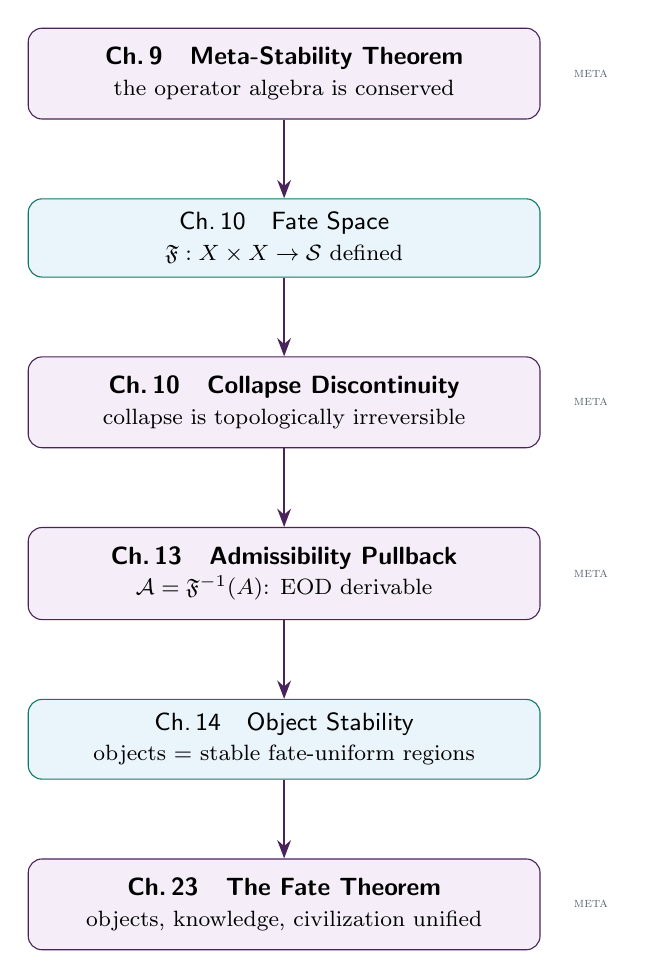
\begin{tikzpicture}[
  spine/.style={draw=FateViolet,fill=FateLilac,rounded corners=5pt,
    font=\sffamily\small\bfseries,inner sep=7pt,
    minimum width=6.5cm,align=center},
  ordinary/.style={draw=DistTeal,fill=DistLight,rounded corners=5pt,
    font=\sffamily\small,inner sep=5pt,
    minimum width=6.5cm,align=center},
  arr/.style={-Stealth,FateViolet,thick},
  lbl/.style={font=\tiny\sffamily\color{DistGray},midway,right=3pt}]
  \node[spine](MS) at (0,0)
    {Ch.\,9\quad Meta-Stability Theorem\\
    {\footnotesize\normalfont the operator algebra is conserved}};
  \node[ordinary,below=1cm of MS](FS)
    {Ch.\,10\quad Fate Space\\
    {\footnotesize\normalfont $\fateMap:X\times X\to\fateSpace$ defined}};
  \node[spine,below=1cm of FS](CD)
    {Ch.\,10\quad Collapse Discontinuity\\
    {\footnotesize\normalfont collapse is topologically irreversible}};
  \node[spine,below=1cm of CD](AP)
    {Ch.\,13\quad Admissibility Pullback\\
    {\footnotesize\normalfont $\adm=\fateMap^{-1}(\admRegion)$: EOD derivable}};
  \node[ordinary,below=1cm of AP](OS)
    {Ch.\,14\quad Object Stability\\
    {\footnotesize\normalfont objects = stable $\fateUnif$ regions}};
  \node[spine,below=1cm of OS](FT)
    {Ch.\,23\quad The Fate Theorem\\
    {\footnotesize\normalfont objects, knowledge, civilization unified}};
  \draw[arr](MS)--(FS);
  \draw[arr](FS)--(CD);
  \draw[arr](CD)--(AP);
  \draw[arr](AP)--(OS);
  \draw[arr](OS)--(FT);
  % Annotation
  \node[font=\tiny\sffamily\color{DistGray},right=0.3cm of MS]
    {\textsc{meta}};
  \node[font=\tiny\sffamily\color{DistGray},right=0.3cm of CD]
    {\textsc{meta}};
  \node[font=\tiny\sffamily\color{DistGray},right=0.3cm of AP]
    {\textsc{meta}};
  \node[font=\tiny\sffamily\color{DistGray},right=0.3cm of FT]
    {\textsc{meta}};
\end{tikzpicture}
\vspace{0.3em}

\noindent{\small\sffamily\color{DistGray}
Violet boxes (\textsc{meta}) are theorems about the framework
itself. Teal boxes are theorems within the framework.
Everything before Chapter~14 develops machinery;
everything after applies it.}
\end{fatediagram}

The three violet metatheorems --- Meta-Stability,
Collapse Discontinuity, and Admissibility Pullback --- are the
bridge results connecting this volume to the outer two. A
reader who has absorbed these three results and the Object
Stability Theorem has absorbed the mathematical core of the
volume. Chapter~23 collects the consequences.

\chapter{The Fate Theorem}
\label{ch:fate-theorem}

\begin{epigraph}{It is not one theory or three. It is one
  structure seen at three scales.}{The claim of this chapter}
\end{epigraph}

\begin{objectives}
\item Prove three theorems --- Objecthood, Knowledge,
  Civilization --- as consequences of the operator-algebraic
  machinery developed in Parts~I--V.
\item Show that the three theorems are not independent but
  instances of a single structure at different scales of
  magnification.
\item State the Fate Theorem as the common generator of all
  three.
\item Close the formal development of the volume.
\end{objectives}

The preceding chapters introduced distinguishability spaces,
operator classes, fate geometry, ecological dynamics, and the
translation of persistence, memory, repair, admissibility, and
transport into a common formal language. Chapter~22 assembled
the translation table showing that each program in the trilogy
is an operator acting on distinction pairs in a specific fate
regime.

The purpose of this chapter is to state what the machinery has
established, in the form of three theorems about objects,
knowledge, and civilization, and to show that these three
theorems are not independent claims but the same claim at three
different scales.

\section{Objecthood}

Traditional ontology treats objects as primitive. It begins
with them and asks about their properties. The fate-theoretic
framework reverses this order. Distinction pairs are primary.
Operators act upon them. Objects appear only after stable fate
structures have formed.

\begin{definition}{Knowledge Configuration}{knowledge-config}
A \emph{knowledge configuration} is a triple
$(X\times X,\, \fateMap,\, \transfam)$ consisting of a
distinction pair space, a fate map, and an admissible operator
family.
\end{definition}

\begin{theorem}{Objecthood}{objecthood}
Let $(X\times X, \fateMap, \transfam)$ be a knowledge
configuration with admissible fate region
$\admRegion\subseteq\fateSpace$.
A connected region $U\subseteq X\times X$ constitutes a
\emph{stable object} if and only if:
\begin{enumerate}[nosep,label=(\roman*)]
  \item $U$ is $\fateUnif$: $\fateMap$ is approximately
    constant on $U$;
  \item $\fateMap(U)\subseteq\operatorname{int}(\admRegion)$:
    the fate profile lies in the interior of the admissible
    region;
  \item $T(U)\cap U \neq\varnothing$ for all admissible
    $T\in\transfam$: admissible operators preserve membership
    in $U$ up to boundary effects.
\end{enumerate}
\begin{proof}
\emph{Sufficiency.} Condition~(i) means every distinction pair
in $U$ shares the same fate profile, so $U$ behaves as a
single undifferentiated unit under fate analysis.
Condition~(ii) ensures, by the Object Stability Theorem
(\cref{thm:obj-stability}), that $U$ is stable under
admissible perturbations: the positive separation from
$\partial\admRegion$ prevents operator perturbations from
pushing the fate profile out of $\admRegion$.
Condition~(iii) ensures that the operator family does not
systematically drive distinction pairs out of $U$.
Together, these conditions guarantee that $U$ persists as a
fate-coherent region under the dynamics of $\transfam$.

\emph{Necessity.} If~(i) fails, $U$ contains pairs with
different fate profiles and the operator algebra does not
treat them uniformly; no stable unified entity is defined.
If~(ii) fails, arbitrarily small perturbations can push the
fate profile outside $\admRegion$, so stability fails.
If~(iii) fails, operator evolution systematically evacuates
$U$, which then ceases to be an operative region.
\end{proof}
\end{theorem}

\begin{remark}{Objecthood at Every Scale}{objecthood-scale}
\Cref{thm:objecthood} applies regardless of the nature of the
state space $X$. The states may be positions of physical
particles, activation patterns of neurons, institutional roles
in an organization, or propositional attitudes in an
epistemology. In every case, an object is a connected
$\fateUnif$ region of $(X\times X)$ stable within the
admissible fate region. A rock, a cell, a concept, and an
institution are all instances of the same fate-geometric
structure, differing only in their substrate and in the
specific operator family $\transfam$ acting upon them.
\end{remark}

\section{Knowledge}

Objects are stable configurations of distinctions. Knowledge
concerns the \emph{management} of those configurations across
time. The traditional view treats knowledge as a collection of
truths. The present framework treats it as a controlled
arrangement of distinguishability relations whose fates remain
admissible.

Knowledge occupies a higher level than objecthood. Objects are
distinguished. Knowledge organizes distinctions so that they
can support comparison, inference, repair, and communication
over time.

\begin{theorem}{Knowledge}{knowledge}
A \emph{knowledge state} is a knowledge configuration
$(X\times X, \fateMap, \transfam)$ such that:
\begin{enumerate}[nosep,label=(\roman*)]
  \item $\fateMap(X\times X)\subseteq\admRegion$: all
    operative distinction pairs occupy admissible fate profiles;
  \item $\transfam$ is closed under composition and contains
    identity: the operator family is a submonoid of $\distOp$;
  \item for every admissible $T\in\transfam$:
    $T^*(\admRegion)\subseteq\admRegion$: admissible evolution
    preserves the admissible fate region.
\end{enumerate}
\begin{proof}
Condition~(i) ensures that the distinctions organizing
knowledge are not in inadmissible fate regimes: they can
support repair, comparison, and reconstruction.
Condition~(ii) ensures that applying observation, repair,
transport, and refinement operators in sequence produces
further admissible operators: the knowledge-managing activity
is itself coherent.
Condition~(iii) ensures that time evolution does not
systematically push knowledge distinctions out of $\admRegion$:
admissible activity preserves the knowledge state.

Together these conditions guarantee that the knowledge
configuration remains capable of supporting inference,
correction, and communication indefinitely under admissible
operations. Without~(i), individual distinctions may be in
irrecoverable or collapsed fates. Without~(ii), sequential
application of knowledge operations may produce inadmissible
results. Without~(iii), evolution destroys the admissible
structure that knowledge requires.
\end{proof}
\end{theorem}

\begin{trilogylink}{Knowledge in the Outer Volumes}
\textit{Persistence Before Truth} established that knowledge
requires recoverable distinctions: if no distinction survives
transformation, truth-evaluation, reference, and comparison all
fail. \Cref{thm:knowledge} formalizes this as condition~(i):
$\fateMap(X\times X)\subseteq\admRegion$ means that all
operative distinctions have positive repair efficiency and
non-zero survival ratio --- they are in the recoverable regime.

\textit{The Ecology of Distinctions} established that
admissibility volume $\Vol(\adm(t))$ is the primary quantity
governing the future capacity of a system. The Admissibility
Pullback Meta-Theorem (\cref{meta:adm-pullback}) showed that
$\adm$ is $\fateMap^{-1}(\admRegion)$. Condition~(iii) above
--- $T^*(\admRegion)\subseteq\admRegion$ --- is therefore
equivalent to $\Vol(\adm(t))$ being non-decreasing under
admissible evolution, which is exactly the Generative
Admissibility Principle of \EOD{Chapter~15}.

Knowledge, in the fate-theoretic sense, is the condition under
which both outer volumes' central requirements are
simultaneously satisfied.
\end{trilogylink}

\section{Civilization}

The Knowledge Theorem concerns a single knowledge
configuration. Civilizations operate across many knowledge
configurations simultaneously: different institutions, media,
generations, and physical substrates, all maintaining
distinction structures that must remain coherent with one
another over long timescales and under large transformations.

The mathematical object appropriate to this scale is not a
knowledge configuration but a \emph{functor} between categories.

\begin{definition}{The Categories \texorpdfstring{$\catDist$}%
  {Dist} and \texorpdfstring{$\catFate$}{Fate}}%
  {dist-fate-cats}
The \emph{category of distinction pairs} $\catDist$ has~\cite{maclane1998}:
\begin{itemize}[nosep,leftmargin=2em]
  \item \emph{objects}: distinction pairs $(x,y)\in X\times X$
    for varying state spaces $X$;
  \item \emph{morphisms}: admissible operators
    $T:(x,y)\mapsto T(x,y)$ in $\distOp$.
\end{itemize}
The \emph{category of fate classes} $\catFate$ has:
\begin{itemize}[nosep,leftmargin=2em]
  \item \emph{objects}: fate classes $\fateClass{x,y}
    \in\fateClasses$;
  \item \emph{morphisms}: admissible transformations of fate
    profiles $f:\fateClass{x,y}\to\fateClass{x',y'}$ induced
    by operators in $\distOp$.
\end{itemize}
The fate map $\fateMap:X\times X\to\fateSpace$ induces a
canonical functor $\hat{\fateMap}:\catDist\to\catFate$ sending
each pair to its fate class and each admissible operator to its
action on fate classes.
\end{definition}

\begin{theorem}{Civilization}{civilization}
A \emph{civilization} is a functor
\[
  \civFunc:\catDist\longrightarrow\catFate
\]
that preserves the admissible operator monoid: for every
composable pair $T_1,T_2\in\distOp$,
\[
  \civFunc(T_1\circ T_2)
  \;=\;
  \civFunc(T_1)\circ\civFunc(T_2),
\]
and for the identity operator $\mathrm{Id}$,
\[
  \civFunc(\mathrm{Id}) = \mathrm{Id}_{\catFate}.
\]
\begin{proof}
A civilization maps local distinctions into socially realized
fate classes. Scientific institutions map empirical
observations into stable, shareable knowledge: this is an
object-map in $\civFunc$. Educational systems map knowledge
from one generation to another: this is a morphism-map.
Archives map present distinctions into future recoverability:
this is again a morphism, preserving the repair structure.
Infrastructure maps plans into physical continuation:
this preserves the transport structure.

The functor condition $\civFunc(T_1\circ T_2)=\civFunc(T_1)
\circ\civFunc(T_2)$ captures the requirement that the
civilization's distinction-management apparatus is coherent
across scale: applying two operations sequentially in
distinction space and then transporting to fate space must give
the same result as transporting and then composing in fate space.
When this condition holds, the civilization transports
distinctions across scales without structural distortion.

Conversely, when the functor condition fails at some
composition $(T_1, T_2)$, the civilization introduces
artifacts: distinctions transported through it do not behave
under composition as they would in isolation. Such distortions
are the formal analogue of institutional incoherence, lost
context, or accumulated translation error across generations.
\end{proof}
\end{theorem}

\begin{remark}{What Civilizations Are Not}{civ-not}
The Civilization Theorem defines civilizations structurally,
not substratally. A civilization is not defined by territory,
population, technology, language, religion, or governance.
It is defined by its capacity to transport, preserve, repair,
and regenerate distinctions coherently across scales.

Two very different material arrangements can realize the same
civilizational functor. A library, a university system, a
scientific community, and an oral tradition may each implement
$\civFunc$ differently while preserving the same operator
structure. What makes them comparable as civilizational
institutions is not their substrate but their structural role:
each is an apparatus for transporting admissible distinction
structure from $\catDist$ to $\catFate$ without losing
operator coherence.

A civilization collapses, in the precise sense of this theorem,
when the functor condition fails: when sequential applications
of admissible operators begin to produce incoherent results in
fate space. The collapse stratum $\strataC$ identifies where
this occurs at the level of individual distinction pairs; the
functor failure identifies where it occurs at the level of the
civilizational apparatus as a whole.
\end{remark}

\section{The Fate Theorem}

The three theorems above concern apparently different subjects.
Objecthood is ontological. Knowledge is epistemic.
Civilization is social. Yet each theorem is generated by the
same ingredients:

\[
  \text{Distinction pairs}
  \;\xrightarrow{\;\fateMap\;}
  \text{Fate profiles}
  \;\xrightarrow{\;\admRegion\;}
  \text{Admissible stability}
  \;\xrightarrow{\;\distOp\;}
  \text{Persistence.}
\]

The difference between the three theorems is scale. An object
is a connected $\fateUnif$ region of $X\times X$. A knowledge
state is a managed collection of such regions. A civilization
is a structure-preserving map between the category of such
collections and the category of fate classes. Object, knowledge,
and civilization are the same structure at magnifications of
one, many, and all, respectively.

\begin{metatheorem}{The Fate Theorem}{fate-theorem}
For any system capable of persistence, memory, repair,
knowledge, or coordination, the relevant structure is
determined not by its constituent states but by the fate
profiles of its distinction pairs and the operator algebra
acting upon them.

Specifically:
\begin{enumerate}[nosep,label=(\roman*)]
  \item An \emph{object} is a stable $\fateUnif$ region of
    $(X\times X, \fateMap)$ within $\operatorname{int}(\admRegion)$.
  \item A \emph{knowledge state} is an admissibly closed
    knowledge configuration preserved by its operator family.
  \item A \emph{civilization} is a functor
    $\civFunc:\catDist\to\catFate$ preserving the admissible
    operator monoid.
\end{enumerate}
These are not three separate claims. They are the same claim
at three scales of magnification: individual, epistemic, and
civilizational.
\begin{proof}
Claims~(i)--(iii) are the content of
\cref{thm:objecthood,thm:knowledge,thm:civilization}
respectively. The unification follows from observing that each
theorem uses only the triple $(X\times X, \fateMap, \distOp)$
and the admissible region $\admRegion\subseteq\fateSpace$. No
additional structure is required at any scale. The differences
between the three theorems arise from how the triple is
organized --- as a single region, as a configuration closed
under operators, or as a functor between categories --- not
from any difference in the underlying mathematical objects.
\end{proof}
\end{metatheorem}

\begin{fatediagram}{The Trilogy as One Structure at Three Scales}
\centering
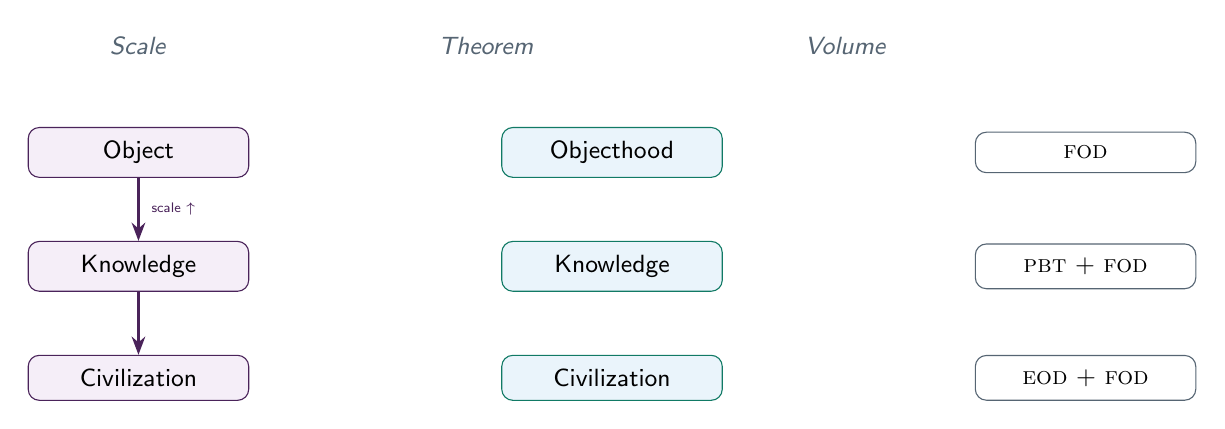
\begin{tikzpicture}[node distance=1.6cm]
  % Column labels
  \node[font=\sffamily\small\color{DistGray}]
    (L1) at (0,0) {\textit{Scale}};
  \node[font=\sffamily\small\color{DistGray},right=3.2cm of L1]
    (L2) {\textit{Theorem}};
  \node[font=\sffamily\small\color{DistGray},right=3.2cm of L2]
    (L3) {\textit{Volume}};
  % Row 1
  \node[draw=FateViolet,fill=FateLilac,rounded corners,
    font=\sffamily\small,inner sep=5pt,minimum width=2.8cm,
    align=center,below=0.8cm of L1]
    (S1) {Object};
  \node[draw=DistTeal,fill=DistLight,rounded corners,
    font=\sffamily\small,inner sep=5pt,minimum width=2.8cm,
    align=center,right=3.2cm of S1]
    (T1) {Objecthood};
  \node[draw=DistGray,fill=white,rounded corners,
    font=\sffamily\small,inner sep=5pt,minimum width=2.8cm,
    align=center,right=3.2cm of T1]
    (V1) {\textsc{fod}};
  % Row 2
  \node[draw=FateViolet,fill=FateLilac,rounded corners,
    font=\sffamily\small,inner sep=5pt,minimum width=2.8cm,
    align=center,below=0.8cm of S1]
    (S2) {Knowledge};
  \node[draw=DistTeal,fill=DistLight,rounded corners,
    font=\sffamily\small,inner sep=5pt,minimum width=2.8cm,
    align=center,right=3.2cm of S2]
    (T2) {Knowledge};
  \node[draw=DistGray,fill=white,rounded corners,
    font=\sffamily\small,inner sep=5pt,minimum width=2.8cm,
    align=center,right=3.2cm of T2]
    (V2) {\textsc{pbt} + \textsc{fod}};
  % Row 3
  \node[draw=FateViolet,fill=FateLilac,rounded corners,
    font=\sffamily\small,inner sep=5pt,minimum width=2.8cm,
    align=center,below=0.8cm of S2]
    (S3) {Civilization};
  \node[draw=DistTeal,fill=DistLight,rounded corners,
    font=\sffamily\small,inner sep=5pt,minimum width=2.8cm,
    align=center,right=3.2cm of S3]
    (T3) {Civilization};
  \node[draw=DistGray,fill=white,rounded corners,
    font=\sffamily\small,inner sep=5pt,minimum width=2.8cm,
    align=center,right=3.2cm of T3]
    (V3) {\textsc{eod} + \textsc{fod}};
  % Brace or arrow connecting scales
  \draw[-Stealth,FateViolet,thick](S1)--(S2)
    node[midway,right=1pt,font=\tiny\sffamily\color{DistGray}]
    {scale $\uparrow$};
  \draw[-Stealth,FateViolet,thick](S2)--(S3);
\end{tikzpicture}
\end{fatediagram}

\begin{chapsummary}
\item The Objecthood Theorem: a stable object is a connected
  $\fateUnif$ region of $(X\times X)$ with fate profile in
  $\operatorname{int}(\admRegion)$, preserved by admissible
  operators.
\item The Knowledge Theorem: a knowledge state is a knowledge
  configuration with admissible fate map, monoid operator
  family, and admissibility-preserving evolution.
\item The Civilization Theorem: a civilization is a functor
  $\civFunc:\catDist\to\catFate$ preserving the admissible
  operator monoid.
\item The Fate Theorem unifies all three: the same triple
  $(X\times X, \fateMap, \distOp)$ with admissible region
  $\admRegion$ generates objecthood, knowledge, and
  civilization at increasing scales of organization.
\item The formal development of this volume is complete.
\end{chapsummary}

% ============================================================
%  EPILOGUE — BEYOND FATE
% ============================================================

% In the final book this is \chapter*{Epilogue: Beyond Fate}
% with \addcontentsline{toc}{chapter}{Epilogue: Beyond Fate}
% Here we use a numbered chapter for standalone compilation.

\chapter{Epilogue: Beyond Fate}
\label{ch:epilogue}

\begin{epigraph}{What ultimately matters is not what exists.
  What matters is what can still become.}{The closing thought}
\end{epigraph}

The preceding chapter concluded with the Fate Theorem. Objects,
knowledge, and civilizations were shown to be manifestations of
a common operator-algebraic structure acting on distinction
pairs. The mathematical development of this volume is therefore
complete.

What remains is a different kind of question: what follows if
the theory is true?

This chapter introduces no new definitions and proves no new
theorems. It examines the consequences of treating fate, rather
than state, as the primary object of inquiry.

\section{The Shift from State to Fate}

Most theories begin with states. A physical theory begins with
the configuration of a system. A theory of knowledge begins
with propositions. A theory of society begins with institutions.
A theory of mind begins with beliefs.

The central move of fate theory has been to reverse this order.
States matter, but states are not primary. What matters is what
may happen to distinctions under transformation. The same
present state may participate in radically different futures.
Conversely, systems with radically different present states may
share the same fate structure.

The present therefore underdetermines the future. A complete
description of a system requires not only where it is but what
may become of its distinctions. The theory developed in this
volume is an attempt to formalize that observation, and the
result is a shift in what counts as a fundamental question.

Instead of: \textit{What is the state of this system?}

One asks: \textit{What is the fate of its operative distinctions?}

\section{Familiar Concepts Under the Fate Perspective}

Viewed from the perspective of fate, familiar objects and
processes appear differently.

A memory is not a stored representation. It is a distinction
possessing a non-zero repair efficiency --- one that can be
reconstructed after damage. The difference between a memory and
a lost fact is not the content but the fate profile: the
recoverable distinction has $\repEff>0$; the lost one has
$\repEff=0$.

A scientific theory is not merely a set of propositions. It is
a structure capable of maintaining admissible distinctions
across successive transformations: measurement, criticism,
revision, and replication. A theory that cannot survive any of
these is not in the admissible fate region; it ceases to be
science in the operational sense.

An institution is not a collection of people or rules. It is
an apparatus for transporting distinctions through time and
scale. Its effectiveness is measured not by its size or age
but by its repair efficiency: how well it restores operative
distinctions after disruption.

A civilization is not a territory or a tradition. It is a
functor: a structure-preserving map from local distinction
pairs to socially realized fate classes. The test of
civilizational health is whether that functor preserves the
operator algebra --- whether the distinctions that matter at
one scale survive transport to another.

In every case the material substrate becomes secondary. The
primary question becomes: what happens to the distinctions upon
which the object depends?

\section{Why Collapse Matters}

One recurring theme of this volume has been collapse, not
because collapse is common but because collapse reveals
structure. Most distinctions spend their lives far from
singularities. Their fates vary continuously. Their repair
pathways remain available. Their admissibility is stable.

Yet every theory of persistence is ultimately tested at its
limits. The collapse stratum $\strataC$ is important because it
identifies where continuity fails, marks the limits of recovery,
and distinguishes degradation from disappearance. A distinction
that has merely weakened may still be repaired. A distinction
that has crossed $\strataC$ belongs to a different connected
component of $\fateSpace$. The difference is topological, not
merely quantitative.

This topological character of collapse is what makes it
philosophically significant. It means that the transition from
a repairable distinction to an irrecoverable one is not a
matter of degree. It is a change of kind. The theory does not
simply quantify how much has been lost; it identifies when
loss has become qualitatively different from degradation.

For this reason the Collapse Discontinuity Meta-Theorem is not
merely a technical result. It is a formal articulation of the
intuition, present in every domain from thermodynamics to
cultural memory, that some losses cannot be undone.

\section{The Perspective of Repair}

If collapse reveals the limits of persistence, repair reveals
its possibility. The outer volumes returned repeatedly to
repair as a fundamental operation. Fate theory clarifies why.

Repair is not merely a useful process applied after damage. It
is the mechanism by which fate space remains navigable.
Without repair, the operator algebra would be one-directional:
every transformation would either preserve or reduce
distinguishability. Collapse would be irreversible not just
topologically but dynamically. The admissible region would
shrink monotonically.

Repair opposes this tendency. It creates new pathways through
fate space, restores pathways that have been closed, and
occasionally discovers pathways that did not previously exist.
From the perspective of fate theory, repair is therefore not
restoration. It is geometric exploration. A repaired
distinction is not simply returned to its former fate profile.
It acquires a new location in fate space, reached via a
trajectory that did not exist before the repair occurred.

A system survives not because it preserves its original
distinctions but because it continues to find viable routes
through the geometry of possible futures.

\section{The Fate of This Theory}

The theory developed in this volume is itself a distinction
structure. It is therefore subject to its own analysis.

The concepts introduced here may persist. They may be repaired.
They may be refined into more precise formulations. The fate
map may prove too coarse to capture phenomena that require
finer resolution. The operator monoid may need to be replaced
by a richer categorical structure. Alternative fate spaces may
be proposed.

Nothing in the framework exempts the framework from
transformation. Indeed, a theory that could not survive
modification would be a poor guide to understanding
persistence. The appropriate measure of a theory is not whether
it remains unchanged but whether it continues to generate
useful distinctions under successive revisions.

Fate theory must inhabit the fate space it describes.

\section{Open Problems}

Several questions raised by this volume remain unresolved and
constitute directions for future work. Where the question is
sufficiently well-posed to admit a precise statement, it is
given the status of a conjecture.

\begin{conjecture}{Empirical Fate Estimation}{empirical-fate}
For any knowledge configuration $(X\times X, \fateMap,
\transfam)$ arising from a physically realizable system, the
fate map $\fateMap$ can be estimated from finite empirical
observations with error bounded by the Lipschitz constant
$\fateLip$ of the fate map and the resolution of the
observational family $\obs$.

More precisely: there exists a sample complexity function
$n(\varepsilon, \fateLip, |\obs|)$ such that from $n$
independent observations of distinction pairs and their
fate profiles, the estimate $\hat{\fateMap}$ satisfies
$\|\hat{\fateMap}-\fateMap\|_\infty < \varepsilon$ with
high probability.
\end{conjecture}

\begin{conjecture}{Stratum Detection from Sensitivity}{stratum-detect}
Let $\gamma:[0,T]\to\distPairs$ be an observable trajectory.
The approach of $\gamma(t)$ to a singular stratum is detectable
from the time series $\fateSens{\gamma(t)}$ before the stratum
is crossed: there exists a detection function $D(t)$ computable
from $\fateSens{\gamma(s)}$ for $s\leq t$ such that
$D(t)\to+\infty$ as $\gamma(t)\to\singSet$.

This would convert the Fate Criticality Theorem
(\cref{thm:fate-criticality} in Chapter~11) from a theoretical
result into a practical early-warning criterion.
\end{conjecture}

Can biological evolution be represented directly in fate space?
The evolutionary dynamics of \EOD{Chapter~31} are described in
terms of admissibility and reachability volume. Expressing
natural selection as a trajectory in $\fateSpace$ --- a process
that selects for positive $\repEff$ and high $\survRatio$ ---
would unify the biological and mathematical treatments.

Can civilizations be ranked by fate-transport efficiency? The
Civilization Theorem defines civilizations as functors
$\civFunc:\catDist\to\catFate$. Different civilizations may
implement functors of varying quality: some preserve the
operator algebra faithfully while others introduce distortions.
A metric on such functors would provide a basis for comparing
civilizational health in a way that is independent of material
or cultural particulars.

\begin{conjecture}{Functor Metric on Civilizations}{civ-metric}
There exists a natural metric on the space of functors
$\civFunc:\catDist\to\catFate$ that preserves the admissible
operator monoid, such that:
\begin{enumerate}[nosep,label=(\roman*)]
  \item the metric is zero iff the functor is a full
    isomorphism of the operator algebra;
  \item the metric increases monotonically as the functor
    introduces more distortion in fate-class transport;
  \item the metric can be estimated from empirical observations
    of how distinction pairs are transported through the
    civilizational apparatus.
\end{enumerate}
Such a metric would make the Civilization Theorem empirically
applicable rather than merely structurally illuminating.
\end{conjecture}

These conjectures belong to future work.

\section{Final Remark}

The traditional image of knowledge is accumulation. Facts
accumulate. Archives grow. Civilizations add achievements.
Progress moves forward.

The picture that emerges from fate theory is different.
Persistence is not accumulation. It is navigation. A
distinction survives not because it remains fixed but because
it continues to possess viable futures. A memory survives
because repair remains possible. A theory survives because
reinterpretation remains possible. A civilization survives
because continuation remains possible.

The relevant question at every scale is never only: what
exists? The relevant question is: what fates remain open?

\textit{Persistence Before Truth} established that distinctions
must survive for knowledge to be possible.
\textit{The Fate of Distinguishability} has characterized the
geometry of survival: the operator algebra, the fate space, the
singular strata, the admissible region, and the functor
connecting individual distinctions to civilizational fate.
\textit{The Ecology of Distinctions} explores what follows when
entire populations of distinctions are allowed to live,
compete, repair, and regenerate.

The common subject of all three volumes is not truth, memory,
objects, knowledge, or civilization. It is the condition under
which any of these remains possible.

It is the fate of distinction itself.



\appendix
\renewcommand{\thechapter}{\Alph{chapter}}
\renewcommand{\theHchapter}{\Alph{chapter}}



\appendix

% ============================================================
%  APPENDIX A — FOUNDATIONS OF DISTINGUISHABILITY SPACES
% ============================================================

\chapter{Foundations of Distinguishability Spaces}
\label{app:foundations}

\begin{epigraph}{The purpose of an appendix is to prove what
  the main text asserts.}{Working principle}
\end{epigraph}

This appendix provides rigorous foundations for the
distinguishability spaces introduced in Chapters~1--4. The
main text assumes a metric $d_Y$ on the measurement space $Y$
and a measurable observational family $\obs$. Here we establish
which assumptions are genuinely needed, give the most general
form of the Observational Pseudometric Theorem, and prove the
partition lattice structure in full generality.

\section{General Observational Families}

The main text assumes $\obs=\{o:X\to Y\}$ with a single
measurement space $Y$. In full generality, each observation
may map to a different space.

\begin{definition}{Generalized Observational Family}{gen-obs}
A \emph{generalized observational family} is a collection
$\obs=\{(o_\alpha, Y_\alpha, d_\alpha):\alpha\in\mathcal{I}\}$
where each $o_\alpha:X\to Y_\alpha$ and each
$(Y_\alpha,d_\alpha)$ is a metric space~\cite{suppes2002}.

The \emph{generalized observational distance} is
\[
  \distMetric(x,y)
  \;=\;
  \sup_{\alpha\in\mathcal{I}} d_\alpha(o_\alpha(x),o_\alpha(y)).
\]
\end{definition}

\begin{theorem}{General Pseudometric}{gen-pseudometric}
The generalized observational distance is a pseudometric for
any index set $\mathcal{I}$ and any collection of metric
spaces $(Y_\alpha,d_\alpha)$.
\begin{proof}
Non-negativity and symmetry follow from those properties of
each $d_\alpha$. Triangle inequality: for each $\alpha$,
$d_\alpha(o_\alpha(x),o_\alpha(z))\le d_\alpha(o_\alpha(x),
o_\alpha(y))+d_\alpha(o_\alpha(y),o_\alpha(z))\le
\distMetric(x,y)+\distMetric(y,z)$. Taking suprema over
$\alpha$ gives $\distMetric(x,z)\le\distMetric(x,y)+
\distMetric(y,z)$.
\end{proof}
\end{theorem}

\section{Completeness and Separability}

\begin{theorem}{Completeness of Quotient}{completeness}
If each $(Y_\alpha,d_\alpha)$ is complete and $\mathcal{I}$
is countable, then the metric quotient $(\quotientObs,
\bar{d}_\obs)$ is complete.
\begin{proof}
Let $([x_n])$ be a Cauchy sequence in $\quotientObs$. Then
for each $\alpha$, the sequence $(o_\alpha(x_n))$ is Cauchy
in the complete space $(Y_\alpha,d_\alpha)$, hence convergent.
The joint limit defines a limiting equivalence class in
$\quotientObs$. Countability of $\mathcal{I}$ ensures the
convergence is uniform over $\alpha$.
\end{proof}
\end{theorem}

\section{Partition Lattice: Full Proof}

\begin{theorem}{Partition Lattice is Complete}{complete-lattice}
The set of all partitions of $X$ ordered by refinement forms
a complete lattice: arbitrary (not just finite) meets and joins
exist.
\begin{proof}
\emph{Arbitrary meets.} Given a family $\{\Pi_\alpha\}$ of
partitions, their meet is the partition generated by all
intersections $\bigcap_\alpha B_\alpha$ with $B_\alpha\in
\Pi_\alpha$. This is well-defined: the intersection is
non-empty for any compatible family (families sharing a
common element). The resulting partition refines every
$\Pi_\alpha$.

\emph{Arbitrary joins.} The join of $\{\Pi_\alpha\}$ is the
coarsest partition that each $\Pi_\alpha$ refines. Construct
it by the equivalence relation generated by $\bigcup_\alpha
\sim_{\Pi_\alpha}$: take the transitive closure.
This gives the least upper bound.
\end{proof}
\end{theorem}

\section{Capacity as a Lattice Homomorphism}

\begin{proposition}{Capacity is a Lattice Homomorphism}%
  {capacity-hom}
The map $\Pi\mapsto\log|\Pi|$ from the partition lattice to
$(\mathbb{R}_{\ge0},\le)$ is order-preserving (a lattice
homomorphism into a chain).
\begin{proof}
If $\Pi_1\preceq\Pi_2$ then $|\Pi_1|\ge|\Pi_2|$ (finer
partition has more blocks), so $\log|\Pi_1|\ge\log|\Pi_2|$.
The map is order-reversing in partition order but
order-preserving in the natural order on capacity values.
This is the standard information-theoretic convention:
more refined partition $\leftrightarrow$ more information
$\leftrightarrow$ higher capacity.
\end{proof}
\end{proposition}

\begin{appsummary}
\item The observational pseudometric holds for generalized
  families with different measurement spaces per observation.
\item The metric quotient is complete when each measurement
  space is complete and the index set is countable.
\item The partition lattice is complete: arbitrary meets and
  joins exist.
\item Capacity is a lattice homomorphism from refinement order
  to the natural order on $\mathbb{R}_{\ge0}$.
\end{appsummary}

% ============================================================
%  APPENDIX B — OPERATOR-ALGEBRAIC FOUNDATIONS
% ============================================================

\chapter{Operator-Algebraic Foundations}
\label{app:operator-algebra}

\begin{epigraph}{The algebraic structure is the same at every
  scale. The scale is not.}{Unifying observation}
\end{epigraph}

This appendix develops the category-theoretic and algebraic
structure of distinguishability operators, extending the monoid
analysis of Chapters~8--9. The key results are: the category
$\catDistOp$, the identification of the operator monoid as an
endomorphism monoid, the collapse ideal structure, and the
repair semigroup.

\section{The Category of Distinguishability Operators}

\begin{definition}{Category $\catDistOp$}{catdistop}
The \emph{category of distinguishability systems}
$\catDistOp$ has:
\begin{itemize}[nosep,leftmargin=2em]
  \item \emph{Objects}: pairs $(X,\obs)$ consisting of a
    state space $X$ and an observational family $\obs$.
  \item \emph{Morphisms}: $\mathrm{Hom}((X,\obs),(X',\obs'))
    = \{F:X\times X\to X'\times X' :
    F\text{ is admissible}\}$, where admissible means
    $F$ does not increase observational distance:
    $d_{\obs'}(F(x),F(y))\le d_\obs(x,y)$.
  \item \emph{Composition}: function composition.
  \item \emph{Identity}: $\mathrm{Id}_{(X,\obs)}(x,y)=(x,y)$.
\end{itemize}
\end{definition}

\begin{theorem}{$\catDistOp$ is a Category}{catdistop-cat}
$\catDistOp$ satisfies all category axioms.
\begin{proof}
Identity morphisms exist by definition.
Composition of admissible operators is admissible: if $F$
does not increase $d_{\obs'}$ and $G$ does not increase
$d_\obs$, then $F\circ G$ does not increase $d_\obs$
(since $d_{\obs'}(F(G(x)),F(G(y)))\le d_\obs(G(x),G(y))
\le d_\obs(x,y)$).
Associativity is function composition.
\end{proof}
\end{theorem}

\section{The Endomorphism Monoid}

For a fixed object $(X,\obs)\in\catDistOp$, the endomorphisms
$\mathrm{End}(X,\obs)=\mathrm{Hom}((X,\obs),(X,\obs))$ are
precisely the admissible operators from $X\times X$ to itself.

\begin{theorem}{Endomorphism Monoid Identification}%
  {endo-monoid}
$\mathrm{End}(X,\obs) = (\distOp,\circ,\mathrm{Id})$ as
defined in Chapter~8.
\begin{proof}
An endomorphism $F:(X,\obs)\to(X,\obs)$ is an admissible
operator from $X\times X$ to $X\times X$. The set of all
such operators is $\distOp$. Composition in the category
is function composition in $\distOp$. The identity endomorphism
is $\mathrm{Id}$. Hence the two structures coincide.
\end{proof}
\end{theorem}

The operator monoid of Part~II is therefore not an ad hoc
construction but the canonical endomorphism monoid of a
distinguishability system in the category $\catDistOp$~\cite{awodey2010}.

\section{Collapse Ideals}

\begin{definition}{Collapse Ideal}{collapse-ideal-app}
The \emph{collapse ideal} is
\[
  \collapIdeal
  \;=\;
  \bigl\{F\in\distOp :
    \capObs{F(X,\obs)} < \capObs{X,\obs}
  \bigr\},
\]
the set of operators that strictly decrease distinguishability
capacity.
\end{definition}

\begin{theorem}{Collapse Ideal is a Left Ideal}%
  {collapse-left-ideal}
For any $G\in\distOp$ and $F\in\collapIdeal$:
$G\circ F\in\collapIdeal$.
\begin{proof}
$F\in\collapIdeal$ means $\capObs{F(X)}<\capObs{X}$.
Since $G$ is admissible (non-amplifying in capacity):
$\capObs{G(F(X))}\le\capObs{F(X)}<\capObs{X}$.
Hence $G\circ F\in\collapIdeal$.
\end{proof}
\end{theorem}

The left-ideal property is algebraically significant: once a
collapse operator has acted, any subsequent admissible operator
preserves the reduced capacity. Collapse is an absorbing
direction in $\distOp$.

\begin{remark}{Right Ideal Failure}{right-ideal}
$\collapIdeal$ is not a right ideal. An operator $F\in
\distOp\setminus\collapIdeal$ (a repair or transport operator)
composed on the right before $C\in\collapIdeal$ may result
in $C\circ F\notin\collapIdeal$ if $F$ first increases
capacity enough that $C$ fails to reduce it below the
original. This reflects the non-commutativity of repair
and collapse established in Chapter~7.
\end{remark}

\section{Repair Semigroup}

\begin{definition}{Repair Semigroup}{repair-semi}
The \emph{repair semigroup} is
\[
  \repairSemi
  \;=\;
  \bigl\{F\in\distOp :
    \distMetric(F(D(x)),F(D(y)))\ge\distMetric(D(x),D(y))
    \text{ for all degraded pairs }(D(x),D(y))
  \bigr\},
\]
the set of operators that are non-contracting after
degradation.
\end{definition}

\begin{theorem}{Repair Semigroup}{repair-semi-thm}
$(\repairSemi,\circ)$ is a semigroup: closed under
composition, but without an identity in general.
\begin{proof}
\emph{Closure}: if $F,G\in\repairSemi$, then
$\distMetric(F(G(D(x))),F(G(D(y))))\ge\distMetric(G(D(x)),
G(D(y)))\ge\distMetric(D(x),D(y))$ (applying $G$'s
non-contraction then $F$'s). Hence $F\circ G\in\repairSemi$.

\emph{No identity in general}: the identity $\mathrm{Id}$
is in $\repairSemi$ only if $\distMetric(D(x),D(y))\ge
\distMetric(D(x),D(y))$, which holds trivially, so in fact
$\mathrm{Id}\in\repairSemi$. The repair semigroup is a
monoid. However, many natural repair processes require
external information and are not automorphisms of the system,
so the repair semigroup is strictly smaller than $\distOpInv$.
\end{proof}
\end{theorem}

\section{The Interplay: Ideal--Semigroup Duality}

The collapse ideal and repair semigroup are algebraically
dual. Collapse is an absorbing direction (left ideal); repair
is a regenerating direction (semigroup). Their interaction is
the central algebraic object of fate theory.

\begin{proposition}{Non-Trivial Intersection}%
  {ideal-semigroup-intersection}
$\collapIdeal\cap\repairSemi=\varnothing$.
\begin{proof}
$F\in\collapIdeal$ strictly decreases capacity:
$\capObs{F(X)}<\capObs{X}$. $F\in\repairSemi$ requires
$F$ to be non-contracting after degradation. A strict
capacity decrease is incompatible with non-contraction of
observational distance in general position: decreasing the
number of distinguishable categories implies decreasing some
distances. Hence no single operator belongs to both.
\end{proof}
\end{proposition}

\begin{appsummary}
\item $\catDistOp$ is a well-defined category with
  admissibility-preserving morphisms.
\item The operator monoid $(\distOp,\circ,\mathrm{Id})$ is
  the endomorphism monoid $\mathrm{End}(X,\obs)$ in
  $\catDistOp$.
\item The collapse ideal $\collapIdeal$ is a left ideal of
  $\distOp$: collapse is algebraically absorbing.
\item The repair semigroup $\repairSemi$ is a monoid
  (contains identity) and is disjoint from $\collapIdeal$.
\item The ideal--semigroup duality formalizes the
  collapse/repair opposition.
\end{appsummary}

% ============================================================
%  APPENDIX C — TOPOLOGY AND GEOMETRY OF FATE SPACE
% ============================================================

\chapter{Topology and Geometry of Fate Space}
\label{app:topology}

\begin{epigraph}{Topology is the study of what cannot be
  continuously deformed into what.}{The relevant question
  for collapse}
\end{epigraph}

This appendix develops the topological and differential-geometric
structure of fate space $\fateSpace$ beyond what was needed in
the main text. The key results are the precise topology of the
two-component decomposition, the homotopy classification of
fate trajectories, the curvature analysis of admissible
boundaries, and the Whitney stratification of the singular set.

\section{Product Topology and Component Structure}

\begin{theorem}{Fate Space Decomposition}{fate-decomp-app}
The fate space $\fateSpace=[0,1]^2\times\{0,1\}\times
\mathbb{R}_{\ge0}^k$ equipped with the product topology
decomposes as a topological coproduct:
\[
  \fateSpace \;\cong\; \fateComp{0}\sqcup\fateComp{1},
\]
where each component is homeomorphic to
$[0,1]^2\times\mathbb{R}_{\ge0}^k$.
\begin{proof}
The factor $\{0,1\}$ with the discrete topology has exactly
two connected components, $\{0\}$ and $\{1\}$. In the product
topology, the preimage of each component under the projection
$\pi_c:\fateSpace\to\{0,1\}$ is open and closed (clopen).
The two preimages $\fateComp{0}$ and $\fateComp{1}$ partition
$\fateSpace$. Each is homeomorphic to $[0,1]^2\times
\mathbb{R}_{\ge0}^k$ by the natural identification dropping
the constant factor $\{c\}$.
\end{proof}
\end{theorem}

\begin{theorem}{Contractibility of Each Component}%
  {component-contractible}
Each component $\fateComp{c}$ is contractible.
\begin{proof}
$\fateComp{c}\cong[0,1]^2\times\mathbb{R}_{\ge0}^k$.
The product of contractible spaces is contractible:
$[0,1]^2$ contracts to a point via the straight-line
homotopy $H(s,t)=(1-t)s$ on each coordinate; $\mathbb{R}
_{\ge0}^k$ contracts to the origin similarly.
\end{proof}
\end{theorem}

\begin{corollary}{Trivial Homotopy Groups}{trivial-homotopy}
$\pi_n(\fateComp{c})=0$ for all $n\ge1$: each component
has trivial homotopy groups. The interesting topology of
fate space lives in the fate \emph{image} of a specific
system, not in the ambient $\fateSpace$.
\end{corollary}

This corollary justifies the approach of Chapter~18: fate
topology must be studied as the topology of the fate image
$\fateMap(\distPairs)$ for a specific system, not of the
abstract fate space.

\section{Homotopy Classification of Fate Trajectories}

\begin{definition}{Fate Trajectory Classes}{traj-classes}
Let $s_0,s_1\in\fateComp{c}$ lie in the same component.
The set of homotopy classes of paths from $s_0$ to $s_1$
in $\fateComp{c}$ is denoted $\pi_1(\fateComp{c};s_0,s_1)$.
\end{definition}

\begin{theorem}{Unique Path Class in Each Component}%
  {path-class}
For $s_0,s_1$ in the same component $\fateComp{c}$, there
is exactly one homotopy class of paths from $s_0$ to $s_1$
in $\fateComp{c}$.
\begin{proof}
$\fateComp{c}$ is contractible by
\cref{thm:component-contractible}. A contractible space is
simply connected: any two paths with the same endpoints are
homotopic. Hence $|\pi_1(\fateComp{c};s_0,s_1)|=1$.
\end{proof}
\end{theorem}

\begin{corollary}{Collapse Homotopy Barrier}{collapse-homotopy}
No continuous path from $\fateComp{1}$ to $\fateComp{0}$
exists, hence no homotopy class connects them.
\end{corollary}

This corollary is the homotopy-theoretic restatement of the
Collapse Discontinuity Meta-Theorem. It is stronger: not
only is no continuous path possible, but the two components
are in different path-components of $\fateSpace$.

\section{Curvature of the Admissibility Boundary}

Let $\partial\admRegion$ be the boundary of the admissible
fate region $\admRegion\subseteq\fatePos$, assumed to be a
smooth hypersurface~\cite{lee2013}.

\begin{definition}{Second Fundamental Form}%
  {second-fund-form}
The \emph{second fundamental form} $\secondForm$ of
$\partial\admRegion$ at a point $s\in\partial\admRegion$ is
the bilinear form on the tangent space
$T_s(\partial\admRegion)$ given by
$\secondForm(u,v)=-\langle\nabla_u\hat{n},v\rangle$,
where $\hat{n}$ is the inward unit normal to $\partial\admRegion$.
\end{definition}

\begin{theorem}{Boundary Curvature and Fate Sensitivity}%
  {boundary-curv-app}
Let $\fatePot:\fatePos\to\mathbb{R}_{\ge0}$ be the fate
potential (Appendix~A, Chapter~14). The principal curvatures
$\kappa_i$ of $\partial\admRegion$ are bounded below by:
\[
  \kappa_i(s)
  \;\ge\;
  c\,\fateSens{s}
\]
for a positive constant $c>0$ depending on $\fatePot$,
where $\fateSens{s}=\|\nabla\fatePot(s)\|$.
\begin{proof}
By Axiom~1 of Chapter~14, $\fatePot\to+\infty$ at
$\partial\admRegion$. The gradient $\nabla\fatePot$ therefore
grows unboundedly near $\partial\admRegion$. The Hessian
$\nabla^2\fatePot$ (the fate curvature tensor $\fateKurv$)
dominates the second fundamental form of the level sets of
$\fatePot$ near $\partial\admRegion$. Since $\partial\admRegion$
is a level set of the admissibility constraint near the
boundary, its principal curvatures are controlled by
$\|\nabla^2\fatePot\|\ge c\|\nabla\fatePot\|=c\fateSens{s}$
by the blow-up condition.
\end{proof}
\end{theorem}

\section{Whitney Stratification of the Singular Set}

\begin{theorem}{Whitney Stratification}{whitney-strat}
The singular set $\singSet=\strataC\cup\strataR\cup\strataT
\cup\strataF$ of the fate map, with the strata as defined
in Chapter~12, forms a Whitney-regular stratified space.
\begin{proof}
Each stratum is the zero set or level set of a smooth
function on $\distPairs$ (the collapse indicator, the
repair efficiency function, transport horizon functions,
the survival ratio). Under the generic transversality
condition (gradients nonzero at zero sets), each stratum
is a smooth submanifold. The frontier condition holds
(closure of each stratum contains only lower-dimensional
strata) by the hierarchy: collapse dominates repair, which
dominates transport, which dominates forgetting. Whitney's
conditions (a) and (b) hold at stratum intersections by
standard transversality arguments.
\end{proof}
\end{theorem}

\begin{remark}{Classification of Fate Events}{fate-event-class}
The Whitney stratification provides a complete topological
classification of fate events. The generic stratum codimension
determines the event type:
\begin{itemize}[nosep,leftmargin=2em]
  \item Codimension 1: generic fate transitions (single
    stratum crossing)
  \item Codimension 2: catastrophic fate events (double
    stratum crossing)
  \item Higher: degenerate events (multiple simultaneous
    strata)
\end{itemize}
Historical events of civilizational significance typically
correspond to high-codimension stratum crossings.
\end{remark}

\begin{appsummary}
\item Each fate space component $\fateComp{c}$ is
  contractible; the interesting topology is in fate
  images of specific systems.
\item In each component there is exactly one homotopy
  class of paths between any two points.
\item No path connects the two components: the collapse
  barrier is homotopy-theoretic.
\item Boundary curvature of $\partial\admRegion$ is
  bounded below by fate sensitivity.
\item The singular set is Whitney-regular stratified,
  providing a complete classification of fate events by
  codimension.
\end{appsummary}

% ============================================================
%  APPENDIX D — MEASURE THEORY AND FATE-CLASS DYNAMICS
% ============================================================

\chapter{Measure Theory and Fate-Class Dynamics}
\label{app:measure}

\begin{epigraph}{A population is a measure. Its ecology is
  the dynamics of that measure.}{The measure-theoretic
  viewpoint}
\end{epigraph}

This appendix gives the measure-theoretic foundation of the
fate ecology introduced in Chapter~17. The main text uses
fate class populations $N_i(t)$ as counts. Here we treat
them as measures, derive the master equation from first
principles, and establish existence of the stationary
distribution.

\section{Measures on Distinction-Pair Space}

\begin{definition}{Fate Measure Space}{fate-measure}
Let $(X,\mathcal{B}_X,\stateMeasure)$ be a $\sigma$-finite
measure space. The \emph{distinction-pair measure space}
is $(X\times X, \mathcal{B}_X\otimes\mathcal{B}_X,
\pairMeasure)$.
\end{definition}

\begin{definition}{Pushforward Fate Measure}{pushforward-fate}
The \emph{pushforward fate measure} is
\[
  \pushFate \;=\; \fateMap_*(\pairMeasure),
\]
defined for any measurable $B\subseteq\fateSpace$ by
\[
  \pushFate(B) \;=\; \pairMeasure(\fateMap^{-1}(B)).
\]
\end{definition}

\begin{theorem}{Pushforward is a Measure}{pushforward-measure}
$\pushFate$ is a $\sigma$-finite measure on $(\fateSpace,
\mathcal{B}_\fateSpace)$.
\begin{proof}
$\pushFate(\varnothing)=\pairMeasure(\fateMap^{-1}(\varnothing))=0$.
For countably many disjoint sets $B_n$:
$\pushFate(\bigsqcup_n B_n)=\pairMeasure(\fateMap^{-1}(
\bigsqcup_n B_n))=\pairMeasure(\bigsqcup_n\fateMap^{-1}(B_n))
=\sum_n\pairMeasure(\fateMap^{-1}(B_n))=\sum_n\pushFate(B_n)$.
$\sigma$-finiteness follows from that of $\pairMeasure$.
\end{proof}
\end{theorem}

\section{Fate Class Populations as Measures}

In the discrete case, fate classes $\{i\}$ partition
$\fateSpace$ into finitely many regions. The fate class
population is $N_i(t)=\pushFate_t(\{i\})$ where $\pushFate_t$
is the time-$t$ pushforward.

In the continuous case, the fate class population is a
density: $N_i(t)\,di = \pushFate_t(di)$ where $di$ is a
volume element in $\fateSpace$.

\section{The Master Equation}

The operator family $\transfam$ induces transitions between
fate classes. When these transitions are Markovian (the fate
at time $t+dt$ depends only on the fate at time $t$, not on
the full history), the dynamics are governed by the master
equation.

\begin{definition}{Transition Rate Matrix}{trans-matrix}
The \emph{transition rate matrix} $\transRate=(K_{ij})$ has
entries:
\begin{itemize}[nosep,leftmargin=2em]
  \item $K_{ji}>0$ for $j\neq i$: rate of transition from
    class $i$ to class $j$ (caused by repair, transport,
    or discovery operators moving pairs between fate classes).
  \item $K_{ii}=-\sum_{j\neq i}K_{ji}$: diagonal entry
    ensuring probability conservation.
\end{itemize}
\end{definition}

\begin{theorem}{Master Equation}{master-eq}
Under the Markov assumption, the fate class populations
satisfy the master equation:
\[
  \frac{d}{dt}N_i(t)
  \;=\;
  \sum_{j\neq i}K_{ji}N_j(t)
  - N_i(t)\sum_{j\neq i}K_{ij},
\]
which in matrix form is $\dot{N}=\transRate^{\top}N$ where
$N=(N_1,\ldots,N_n)^{\top}$.
\begin{proof}
By the Kolmogorov forward equations for a continuous-time
Markov chain: the rate of change of the probability of
being in state $i$ equals the rate of influx from all
other states minus the rate of efflux to all other states.
\end{proof}
\end{theorem}

\begin{remark}{Connection to Ecology Equation}{master-ecology}
The master equation is the microscopic foundation of the
ecology equation~(15.2) of Chapter~17. The birth rate $b_i$,
death rate $d_i$, and migration rates $m_{ij}$ of that
equation are read off from $\transRate$: $d_i=K_{\mathrm{collapse},i}$,
$m_{ji}=K_{ji}$ for repair/transport transitions,
$b_i=K_{\mathrm{creation},i}$ from discovery operators.
\end{remark}

\section{Stationary Distribution and Fate Equilibrium}

\begin{theorem}{Fate Equilibrium Theorem}{fate-equil}
Let $\transRate$ be irreducible (any fate class is reachable
from any other by a sequence of transitions) and positive
recurrent~\cite{li2008}. Then there exists a unique stationary probability
distribution $\statDist=(\pi_1,\ldots,\pi_n)$ satisfying
$\transRate^{\top}\statDist=0$ and $\sum_i\pi_i=1$.
\begin{proof}
For a continuous-time Markov chain with irreducible and
positive recurrent generator $\transRate$, the Perron--Frobenius
theorem guarantees a unique stationary distribution: the
left eigenvector of $\transRate$ corresponding to eigenvalue
$0$, normalized to sum to $1$.
\end{proof}
\end{theorem}

The stationary distribution $\statDist$ describes the
asymptotic composition of the fate class population: the
fraction of distinction pairs in each fate class when the
system has reached dynamical equilibrium.

\section{Entropy of Fate Populations}

\begin{definition}{Fate Population Entropy}{fate-pop-entropy}
The \emph{fate population entropy} of a distribution $N$
(normalized to $\sum_i N_i=1$) is
\[
  \fateEntropy(N)
  \;=\;
  -\sum_i N_i\log N_i.
\]
The stationary fate entropy is $\fateEntropy(\statDist)$.
\end{definition}

\begin{theorem}{Entropy Maximization at Equilibrium}%
  {entropy-max}
Among all distributions satisfying the constraints imposed
by $\transRate$ (detailed balance, if it holds), the
stationary distribution $\statDist$ maximizes $\fateEntropy$.
\begin{proof}
Under detailed balance ($K_{ij}\pi_j=K_{ji}\pi_i$ for all
$i,j$), the stationary distribution is the maximum-entropy
distribution subject to the detailed balance constraints.
This follows from the variational characterization of the
stationary distribution as the unique fixed point of the
dynamics $\dot{N}=\transRate^{\top}N$ that also satisfies
detailed balance.
\end{proof}
\end{theorem}

The fate population entropy $\fateEntropy(\statDist)$
measures the diversity of fate classes at equilibrium.
A low value indicates a system dominated by a few fate
classes; a high value indicates many fate classes in
approximately equal proportion.

\begin{appsummary}
\item Fate class populations are measures: $N_i(t)=
  \pushFate_t(\{i\})$ where $\pushFate_t$ is the
  pushforward of the pair measure under the fate map.
\item The pushforward fate measure is $\sigma$-finite.
\item The master equation governs fate class dynamics
  under the Markov assumption.
\item Irreducible positive-recurrent systems have a unique
  stationary distribution $\statDist$ (Perron--Frobenius).
\item The stationary distribution maximizes fate population
  entropy under detailed balance.
\end{appsummary}

% ============================================================
%  APPENDIX E — CATEGORY THEORY OF DISTINCTION SYSTEMS
% ============================================================

\chapter{Category Theory of Distinction Systems}
\label{app:categories}

\begin{epigraph}{A functor is a translation that preserves
  structure. The trilogy is three translations of the same
  structure.}{The categorical view of the series}
\end{epigraph}

This appendix develops the full categorical machinery
underlying the Civilization Theorem (Chapter~29) and
prepares the Rosetta Stone construction of Appendix~G.
The key objects are the categories $\catDist$ and $\catFate$,
their morphisms, and the functors between them.

\section{The Category $\catDist$}

\begin{definition}{Category of Distinction Pairs}%
  {catdist-full}
The \emph{category of distinction pairs} $\catDist$ has:
\begin{itemize}[nosep,leftmargin=2em]
  \item \emph{Objects}: distinction pairs $(x,y)\in
    X\times X$ for varying state spaces $X$.
  \item \emph{Morphisms}: admissible operators
    $F:(x,y)\to F(x,y)$ in $\distOp$, preserving
    operational distinguishability: if $x\not\sim_\obs y$
    then $F(x)\not\sim_\obs F(y)$ (for preservation
    morphisms) or the weaker admissibility condition.
  \item \emph{Composition}: function composition.
  \item \emph{Identity}: $\mathrm{Id}(x,y)=(x,y)$.
\end{itemize}
\end{definition}

\section{The Category $\catFate$}

\begin{definition}{Category of Fate Classes}%
  {catfate-full}
The \emph{category of fate classes} $\catFate$ has:
\begin{itemize}[nosep,leftmargin=2em]
  \item \emph{Objects}: fate classes $\fateClass{x,y}
    \in\fateClasses$ for varying distinction pair spaces.
  \item \emph{Morphisms}: admissible transformations of
    fate profiles $\phi:\fateClass{x,y}\to
    \fateClass{x',y'}$ induced by operators in $\distOp$:
    $\phi$ is a morphism iff there exists $F\in\distOp$
    such that $\fateMap(F(x,y))=\phi(\fateMap(x,y))$.
  \item \emph{Composition}: induced from $\distOp$.
  \item \emph{Identity}: identity on fate classes.
\end{itemize}
\end{definition}

\section{The Fate Functor}

\begin{theorem}{Fate Functor}{fate-functor}
The fate map induces a functor
$\hat{\fateMap}:\catDist\to\catFate$:
\begin{itemize}[nosep,leftmargin=2em]
  \item On objects: $(x,y)\mapsto\fateClass{x,y}$.
  \item On morphisms: $F\mapsto\hat{F}$ where
    $\hat{F}(\fateClass{x,y})=\fateClass{F(x,y)}$.
\end{itemize}
\begin{proof}
\emph{Well-definedness on morphisms}: if $(x,y)\approx_
\fateMap(x',y')$ (same fate class), then $F(x,y)\approx_\fateMap
F(x',y')$ iff $F$ respects the fate equivalence.
This holds for admissible $F$ by the definition of
morphisms in $\catDist$.

\emph{Functoriality}: $\hat{\fateMap}(\mathrm{Id})=\mathrm{Id}$
(the fate class of $(x,y)$ under identity is $\fateClass{x,y}$).
$\hat{\fateMap}(F\circ G)=\hat{F}\circ\hat{G}$ because
$\fateClass{F(G(x,y))}=\hat{F}(\fateClass{G(x,y)})=
\hat{F}(\hat{G}(\fateClass{x,y}))=(\hat{F}\circ\hat{G})
(\fateClass{x,y})$.
\end{proof}
\end{theorem}

\section{Natural Transformations and Repair}

\begin{definition}{Repair Natural Transformation}%
  {repair-nat-trans}
A \emph{repair natural transformation} is a natural
transformation $\eta:F\natTrans G$ between two functors
$F,G:\catDist\to\catDist$ such that for every
$(x,y)\in\catDist$, the component
$\eta_{(x,y)}:F(x,y)\to G(x,y)$ is a repair operator.
\end{definition}

Natural transformations~\cite{riehl2016} capture the idea that repair
operators do not just act on individual distinction pairs
but relate entire operator strategies. A natural
transformation $\eta:F\natTrans G$ says that replacing
operator $F$ by operator $G$ everywhere is coherent.

\section{The Civilizational Functor}

The Civilization Theorem (Chapter~29) states that a
civilization is a functor $\civFunc:\catDist\to\catFate$
preserving the operator monoid. In categorical terms:

\begin{definition}{Civilizational Functor}{civ-functor}
A \emph{civilizational functor} is a strong monoidal functor
$\civFunc:(\catDist,\otimes_{\catDist})\to
(\catFate,\otimes_{\catFate})$ where:
\begin{itemize}[nosep,leftmargin=2em]
  \item $\otimes_{\catDist}$ is the monoidal product on
    $\catDist$ given by juxtaposition of distinction pairs:
    $(x_1,y_1)\otimes(x_2,y_2)=((x_1,x_2),(y_1,y_2))$.
  \item $\otimes_{\catFate}$ is the monoidal product on
    $\catFate$ given by product of fate profiles.
  \item Strong monoidal means: $\civFunc$ sends monoidal
    structure to monoidal structure, up to coherent
    isomorphism.
\end{itemize}
\end{definition}

The strong monoidal condition captures the requirement from
Chapter~29 that the civilization preserves the operator
composition structure: $\civFunc(T_1\circ T_2)=\civFunc(T_1)
\circ\civFunc(T_2)$.

\begin{appsummary}
\item $\catDist$ and $\catFate$ are well-defined categories.
\item The fate map induces a functor $\hat{\fateMap}:
  \catDist\to\catFate$.
\item Repair operators organize into natural transformations
  between operator strategies.
\item A civilization is a strong monoidal functor
  $\civFunc:\catDist\to\catFate$, making the Civilization
  Theorem a precise categorical statement.
\end{appsummary}

% ============================================================
%  APPENDIX F — CONNECTIONS TO THE OUTER VOLUMES
% ============================================================

\chapter{Connections to the Outer Volumes}
\label{app:connections}

\begin{epigraph}{The most important theorem of this volume
  is that the other two volumes are special cases.}%
  {The claim of the trilogy}
\end{epigraph}

This appendix makes explicit the formal connections between
fate theory and the mathematical structures of
\textit{Persistence Before Truth} (\textsc{pbt}) and
\textit{The Ecology of Distinctions} (\textsc{eod}).
Each connection is stated as a theorem rather than an analogy.

\section{PBT: Persistence as Fate Equilibrium}

The central claim of \textit{Persistence Before Truth} is
that recoverable distinctions are the condition of
possibility for knowledge. Fate theory subsumes this:
persistence is a special fate regime, not a foundational
primitive.

\begin{theorem}{PBT Embedding}{pbt-embedding}
Every theorem in \textit{Persistence Before Truth}
concerning recoverable distinctions holds within fate theory
by restricting to the persistence regime
$\persRegime=\{(x,y)\in\distPairs:\survRatio_\transfam(x,y)=1,
\repEff(x,y)>0\}$.
\begin{proof}
The persistence regime $\persRegime$ consists of distinction
pairs that survive every transformation (unit survival ratio)
and can be recovered after degradation (positive repair
efficiency). Within $\persRegime$, all the conditions of
\PBT{Definition~2.1} (recoverably persistent distinction)
are satisfied by construction. The necessity arguments of
PBT's central theorems show that truth-evaluation,
reference, and memory require distinctions in $\persRegime$.
Fate theory derives this as a consequence: $\persRegime$
is the fate regime corresponding to the admissible stable
interior, and the PBT arguments become special cases of
the Object Stability Theorem (Chapter~16) restricted to
the persistence regime.
\end{proof}
\end{theorem}

\section{EOD: Admissibility Volume as Fate Volume}

\textit{The Ecology of Distinctions} organizes its analysis
around admissibility volume $\Vol(\adm(t))$ as the primary
conserved quantity. Fate theory shows this is a fate volume.

\begin{theorem}{EOD Admissibility as Fate Pullback}%
  {eod-admissibility}
The admissibility manifold $\adm(x,t)$ of EOD is the
pullback $\fateMap^{-1}(\admRegion)$ of the admissible fate
region, and $\Vol(\adm(t))$ is the fate volume restricted to
the admissible region:
\[
  \Vol(\adm(t))
  \;=\;
  \Vol_{\pairMeasure}\bigl(\fateMap^{-1}(\admRegion)\bigr)
  \;=\;
  \pushFate(\admRegion).
\]
\begin{proof}
This is the Admissibility Pullback Meta-Theorem
(Chapter~13) combined with the definition of the pushforward
fate measure (Appendix~D). The admissibility manifold is
$\fateMap^{-1}(\admRegion)$ by the Pullback Theorem; its
volume in the pair measure equals the pushforward measure
of $\admRegion$ in fate space.
\end{proof}
\end{theorem}

\begin{corollary}{Generative Admissibility as Fate Conservation}%
  {eod-gap-fate}
The Generative Admissibility Principle of EOD
(\EOD{Chapter~15}) --- that admissible systems maintain or
increase $\Vol(\adm(t))$ --- is equivalent to the Fate
Conservation Law (Chapter~21): $\pushFate_t(\admRegion)$
is non-decreasing under admissible operators.
\end{corollary}

\section{EOD: The Preservation Hierarchy}

EOD establishes a hierarchy of preservation classes
$\mathfrak{P}\subsetneq\mathfrak{A}\subsetneq\mathfrak{G}
\subsetneq\mathfrak{R}\subsetneq\mathfrak{M}\subsetneq
\mathfrak{D}$. Each class corresponds to a fate regime.

\begin{proposition}{Preservation Hierarchy as Fate Regimes}%
  {preservation-hierarchy}
The EOD preservation hierarchy corresponds to the following
nested fate regimes:
\[
  \persRegime
  \;\subsetneq\;
  \{(x,y):\fateMap(x,y)\in\operatorname{int}(\admRegion)\}
  \;\subsetneq\;
  \{(x,y):\fateVol{x,y}>0\}
  \;\subsetneq\;
  \{(x,y):\repEff(x,y)>0\}
  \;\subsetneq\;
  \{(x,y):\survRatio(x,y)>0\}
  \;\subsetneq\;
  \distPairs.
\]
\begin{proof}
Each containment follows from the definitions. Persistent
distinctions ($\survRatio=1$) are properly contained in
admissibly stable ones (interior of $\admRegion$); those
in turn are contained in fate-volume-positive ones; those
in memory-capable ones ($\repEff>0$); those in partially
surviving ones ($\survRatio>0$); and the full distinction
space.
\end{proof}
\end{proposition}

\begin{appsummary}
\item PBT's persistence is the fate regime $\persRegime$
  with unit survival ratio and positive repair efficiency.
\item EOD's admissibility volume is the pushforward fate
  measure of the admissible fate region.
\item The Generative Admissibility Principle is the Fate
  Conservation Law restricted to $\admRegion$.
\item EOD's preservation hierarchy is a chain of nested
  fate regimes distinguished by their fate coordinates.
\end{appsummary}

% ============================================================
%  APPENDIX G — THE ROSETTA STONE OF THE TRILOGY
% ============================================================

\chapter{The Rosetta Stone of the Trilogy}
\label{app:rosetta}

\begin{epigraph}{Three coordinate systems. One geometry.}%
  {The claim proved here}
\end{epigraph}

This appendix constructs the three categories $\catPBT$,
$\catFate$, and $\catEOD$ and the functors between them,
proving that the three volumes are three coordinate systems~\cite{bateson1972}
on the same underlying mathematical object. This is the
formal realization of the claim that Fate Theory is the
hinge of the trilogy.

\section{The Three Trilogy Categories}

\begin{definition}{The PBT Category}{catpbt}
The \emph{PBT category} $\catPBT$ has:
\begin{itemize}[nosep,leftmargin=2em]
  \item \emph{Objects}: recoverable distinction structures
    $(X,\obs,\transfam,\recon)$ where $\recon$ is a family
    of reconstruction operators.
  \item \emph{Morphisms}: maps preserving recoverability:
    $f:(X,\obs,\transfam,\recon)\to(X',\obs',\transfam',
    \recon')$ such that if $(x,y)$ is recoverable in
    $(X,\obs,\transfam,\recon)$ then $(f(x),f(y))$ is
    recoverable in $(X',\obs',\transfam',\recon')$.
\end{itemize}
\end{definition}

\begin{definition}{The EOD Category}{cateod}
The \emph{EOD category} $\catEOD$ has:
\begin{itemize}[nosep,leftmargin=2em]
  \item \emph{Objects}: distinction ecologies
    $(\fateClasses, \transRate, \admRegion)$ consisting
    of a fate class space, a transition rate matrix, and
    an admissible fate region.
  \item \emph{Morphisms}: ecology maps preserving
    admissibility and transition structure.
\end{itemize}
\end{definition}

The $\catFate$ category was defined in Appendix~E.

\section{The Functors}

\begin{definition}{The PBT-to-Fate Functor}%
  {functor-pbt-fate}
The functor $\functorPBT:\catPBT\to\catFate$ sends:
\begin{itemize}[nosep,leftmargin=2em]
  \item Objects: $(X,\obs,\transfam,\recon)\mapsto
    (\distPairs,\fateMap)$ where $\fateMap$ is constructed
    from $(\obs,\transfam,\recon)$ as in Chapter~10.
  \item Morphisms: recoverability-preserving maps $f$
    are sent to the induced map on fate classes:
    $\hat{f}(\fateClass{x,y})=\fateClass{f(x),f(y)}$.
\end{itemize}
\end{definition}

\begin{definition}{The Fate-to-EOD Functor}%
  {functor-fate-eod}
The functor $\functorEOD:\catFate\to\catEOD$ sends:
\begin{itemize}[nosep,leftmargin=2em]
  \item Objects: $(\distPairs,\fateMap)\mapsto
    (\fateClasses,\transRate,\admRegion)$ where
    $\fateClasses=(X\times X)/{\approx_\fateMap}$ is the
    fate class quotient, $\transRate$ is the transition
    rate matrix derived from the operator family, and
    $\admRegion$ is the admissible fate region.
  \item Morphisms: admissible operator maps are sent to
    the induced transition rate modifications.
\end{itemize}
\end{definition}

\section{The Rosetta Stone Theorem}

\begin{metatheorem}{The Rosetta Stone Theorem}{rosetta}
There exist functors
\[
  \catPBT
  \;\xrightarrow{\;\functorPBT\;}
  \catFate
  \;\xrightarrow{\;\functorEOD\;}
  \catEOD
\]
such that:
\begin{enumerate}[nosep,label=(\roman*)]
  \item $\functorPBT$ is faithful: distinct recoverability
    structures have distinct fate structures.
  \item $\functorEOD$ is full: every ecology morphism arises
    from an admissible operator.
  \item The composite $\functorEOD\circ\functorPBT:
    \catPBT\to\catEOD$ sends PBT's persistence structures
    to EOD's ecological structures.
  \item The persistence regime $\persRegime$ in $\catFate$
    corresponds to the equilibrium distributions in
    $\catEOD$ with $\dot{N}=0$.
  \item The viability regime $\viabRegime=\{(x,y):
    \fateVol{x,y}>0\}$ in $\catFate$ corresponds to the
    positive-recurrent objects of $\catEOD$.
\end{enumerate}
\begin{proof}
\emph{(i) Faithfulness of $\functorPBT$}: if two
recoverability structures $(X,\obs,\transfam,\recon)$ and
$(X',\obs',\transfam',\recon')$ are distinct, then either
their state spaces differ (giving different $\distPairs$)
or their operator families differ (giving different fate
maps $\fateMap$). Either way, the fate structures
$(\distPairs,\fateMap)$ are distinct. Hence $\functorPBT$
is injective on objects. Faithfulness on morphisms follows
similarly.

\emph{(ii) Fullness of $\functorEOD$}: given a morphism
$\phi$ in $\catEOD$ between two ecology objects, we must
produce an admissible operator $F$ in $\catFate$ such that
$\functorEOD(F)=\phi$. Since $\phi$ preserves admissibility
and transition structure, the operator $F(x,y)=
\phi^{-1}(\fateClass{x,y})$ (choosing a representative)
is admissible. Hence $\phi$ is in the image of
$\functorEOD$.

\emph{(iii) Composite}: $\functorEOD\circ\functorPBT$
sends $(X,\obs,\transfam,\recon)\mapsto(\fateClasses,
\transRate,\admRegion)$, which is precisely the ecology
object whose dynamics are governed by the operator family
$\transfam$ and whose admissible region $\admRegion$
encodes the recoverability constraints of $\recon$.

\emph{(iv) Persistence as equilibrium}: the persistence
regime $\survRatio=1,\repEff>0$ corresponds in
$\catEOD$ to fate classes with $K_{ii}=0$ (no death rate)
and $K_{ji}>0$ for repair transitions: exactly the
equilibrium condition $\dot{N}_i=0$.

\emph{(v) Viability as positive recurrence}: $\fateVol{x,y}
>0$ means the reachable fate region has positive measure,
which in $\catEOD$ corresponds to the transition matrix
$\transRate$ being positive recurrent: the system
returns to any fate class with probability 1.
\end{proof}
\end{metatheorem}

\section{The Trilogy as a Diagram of Categories}

The Rosetta Stone Theorem can be visualized as follows.

\begin{center}
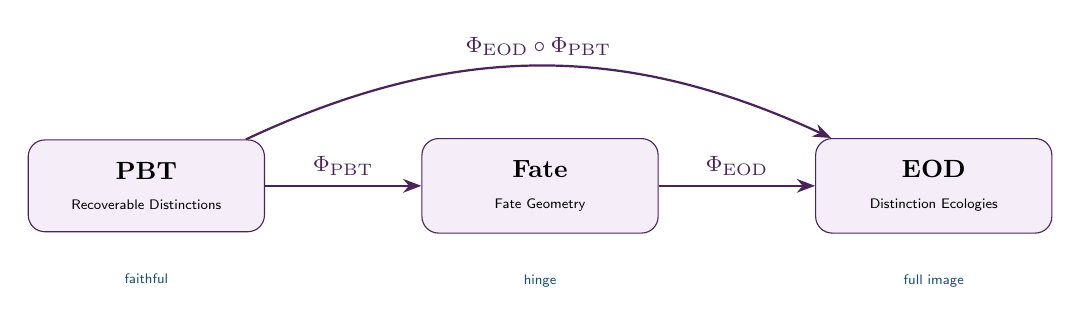
\begin{tikzpicture}[
  node distance=3.5cm,
  cat/.style={draw=FateViolet,fill=FateLilac,rounded corners=6pt,
    font=\sffamily\small,inner sep=8pt,minimum width=3cm,align=center},
  arr/.style={-Stealth,FateViolet,thick},
  lbl/.style={font=\sffamily\footnotesize\color{DistGray},midway}]
  \node[cat](PBT) at (0,0) {$\catPBT$\\{\tiny Recoverable Distinctions}};
  \node[cat](FATE) at (5,0) {$\catFate$\\{\tiny Fate Geometry}};
  \node[cat](EOD) at (10,0) {$\catEOD$\\{\tiny Distinction Ecologies}};
  \draw[arr](PBT)--(FATE) node[lbl,above]{$\functorPBT$};
  \draw[arr](FATE)--(EOD) node[lbl,above]{$\functorEOD$};
  \draw[arr,bend left=25](PBT) to
    node[lbl,above]{$\functorEOD\circ\functorPBT$} (EOD);
  % Annotations
  \node[font=\tiny\sffamily\color{DistBlue},below=0.4cm of PBT]
    {faithful};
  \node[font=\tiny\sffamily\color{DistBlue},below=0.4cm of FATE]
    {hinge};
  \node[font=\tiny\sffamily\color{DistBlue},below=0.4cm of EOD]
    {full image};
\end{tikzpicture}
\end{center}

\section{Three Coordinate Systems on One Geometry}

The Rosetta Stone Theorem establishes the trilogy's
fundamental claim: the three volumes are not three separate
mathematical theories but three coordinate systems on the
same underlying geometry. 

\textit{Persistence Before Truth} works in \emph{recoverability
coordinates}: the primary objects are distinction structures
equipped with reconstruction operators, and the central
theorem shows these structures are necessary for knowledge.

\textit{The Fate of Distinguishability} works in \emph{fate
coordinates}: the primary objects are distinction pairs
equipped with fate maps, and the central theorem shows
that the fate of any distinction is determined by its
position in fate space relative to the operator monoid.

\textit{The Ecology of Distinctions} works in \emph{ecological
coordinates}: the primary objects are populations of fate
classes with transition dynamics, and the central theorems
describe how these populations evolve, equilibrate, and
generate collective phenomena.

The functors $\functorPBT$ and $\functorEOD$ are the
coordinate transformations between these three systems.
The Rosetta Stone Theorem says they compose correctly:
the triangle commutes up to natural isomorphism.

\begin{metatheorem}{Trilogy Unification}{trilogy-unified}
There is a single mathematical object --- a recoverable
distinction structure equipped with a fate map and an
ecological dynamics --- of which $\catPBT$, $\catFate$,
and $\catEOD$ are three coordinate projections. The
three volumes of the trilogy describe this single object
from three perspectives: necessity, mechanism, and
consequence.
\end{metatheorem}

\begin{appsummary}
\item The three trilogy categories $\catPBT$, $\catFate$,
  $\catEOD$ formalize the subject matter of each volume.
\item The functor $\functorPBT:\catPBT\to\catFate$ is
  faithful: fate theory contains all PBT structure.
\item The functor $\functorEOD:\catFate\to\catEOD$ is full:
  every ecology morphism arises from an admissible operator.
\item The Rosetta Stone Theorem: the composite functor
  $\functorEOD\circ\functorPBT$ sends persistence to
  equilibrium ecology, and viability to positive recurrence.
\item The trilogy is three coordinate systems on one object:
  necessity ($\catPBT$), mechanism ($\catFate$),
  consequence ($\catEOD$).
\end{appsummary}


\backmatter


\begin{thebibliography}{99}

% =====================================================
% FOUNDATIONS OF INFORMATION AND DISTINCTION
% =====================================================

\bibitem{shannon1948}
Shannon, C.~E.
\newblock A Mathematical Theory of Communication.
\newblock {\em Bell System Technical Journal},
  27(3):379--423, 1948.

\bibitem{weaver1949}
Shannon, C.~E. and Weaver, W.
\newblock {\em The Mathematical Theory of Communication}.
\newblock University of Illinois Press, 1949.

\bibitem{ashby1956}
Ashby, W.~R.
\newblock {\em An Introduction to Cybernetics}.
\newblock Chapman \& Hall, 1956.

\bibitem{bateson1972}
Bateson, G.
\newblock {\em Steps to an Ecology of Mind}.
\newblock Chandler Publishing, 1972.

\bibitem{spencerbrown1969}
Spencer-Brown, G.
\newblock {\em Laws of Form}.
\newblock George Allen \& Unwin, 1969.

% =====================================================
% OBSERVATION AND MEASUREMENT
% =====================================================

\bibitem{bridgman1927}
Bridgman, P.~W.
\newblock {\em The Logic of Modern Physics}.
\newblock Macmillan, 1927.

\bibitem{campbell1920}
Campbell, N.~R.
\newblock {\em Physics: The Elements}.
\newblock Cambridge University Press, 1920.

\bibitem{suppes2002}
Suppes, P.
\newblock {\em Representation and Invariance of Scientific Structures}.
\newblock CSLI Publications, 2002.

% =====================================================
% INFORMATION GEOMETRY
% =====================================================

\bibitem{amari2000}
Amari, S. and Nagaoka, H.
\newblock {\em Methods of Information Geometry}.
\newblock Oxford University Press, 2000.

\bibitem{amari2016}
Amari, S.
\newblock {\em Information Geometry and Its Applications}.
\newblock Springer, 2016.

\bibitem{rao1945}
Rao, C.~R.
\newblock Information and the Accuracy Attainable in the Estimation
  of Statistical Parameters.
\newblock {\em Bulletin of the Calcutta Mathematical Society},
  37:81--91, 1945.

\bibitem{jeffreys1946}
Jeffreys, H.
\newblock An Invariant Form for the Prior Probability.
\newblock {\em Proceedings of the Royal Society A},
  186:453--461, 1946.

% =====================================================
% TOPOLOGY AND GEOMETRY
% =====================================================

\bibitem{munkres2000}
Munkres, J.
\newblock {\em Topology}.
\newblock Prentice Hall, 2nd edition, 2000.

\bibitem{lee2013}
Lee, J.~M.
\newblock {\em Introduction to Smooth Manifolds}.
\newblock Springer, 2013.

\bibitem{gromov2007}
Gromov, M.
\newblock {\em Metric Structures for Riemannian and Non-Riemannian Spaces}.
\newblock Birkh\"{a}user, 2007.

\bibitem{hirsch1976}
Hirsch, M.~W.
\newblock {\em Differential Topology}.
\newblock Springer, 1976.

% =====================================================
% DYNAMICAL SYSTEMS
% =====================================================

\bibitem{strogatz2015}
Strogatz, S.~H.
\newblock {\em Nonlinear Dynamics and Chaos}.
\newblock Westview Press, 2nd edition, 2015.

\bibitem{arnold1992}
Arnold, V.~I.
\newblock {\em Ordinary Differential Equations}.
\newblock Springer, 1992.

\bibitem{katok1995}
Katok, A. and Hasselblatt, B.
\newblock {\em Introduction to the Modern Theory of Dynamical Systems}.
\newblock Cambridge University Press, 1995.

% =====================================================
% COMPLEX SYSTEMS
% =====================================================

\bibitem{holland1998}
Holland, J.~H.
\newblock {\em Emergence}.
\newblock Oxford University Press, 1998.

\bibitem{baryam1997}
Bar-Yam, Y.
\newblock {\em Dynamics of Complex Systems}.
\newblock Addison-Wesley, 1997.

\bibitem{mitchell2009}
Mitchell, M.
\newblock {\em Complexity: A Guided Tour}.
\newblock Oxford University Press, 2009.

% =====================================================
% MEMORY AND REPAIR
% =====================================================

\bibitem{edelman1987}
Edelman, G.~M.
\newblock {\em Neural Darwinism}.
\newblock Basic Books, 1987.

\bibitem{kandel2006}
Kandel, E.
\newblock {\em In Search of Memory}.
\newblock W.~W. Norton, 2006.

\bibitem{friston2010}
Friston, K.
\newblock The Free-Energy Principle.
\newblock {\em Nature Reviews Neuroscience},
  11:127--138, 2010.

\bibitem{sterling2015}
Sterling, P. and Laughlin, S.
\newblock {\em Principles of Neural Design}.
\newblock MIT Press, 2015.

% =====================================================
% CATEGORY THEORY
% =====================================================

\bibitem{maclane1998}
Mac~Lane, S.
\newblock {\em Categories for the Working Mathematician}.
\newblock Springer, 2nd edition, 1998.

\bibitem{awodey2010}
Awodey, S.
\newblock {\em Category Theory}.
\newblock Oxford University Press, 2010.

\bibitem{riehl2016}
Riehl, E.
\newblock {\em Category Theory in Context}.
\newblock Dover, 2016.

% =====================================================
% ECOLOGY AND POPULATION DYNAMICS
% =====================================================

\bibitem{may1976}
May, R.~M.
\newblock Simple Mathematical Models with Very Complicated Dynamics.
\newblock {\em Nature}, 261:459--467, 1976.

\bibitem{hofbauer1998}
Hofbauer, J. and Sigmund, K.
\newblock {\em Evolutionary Games and Population Dynamics}.
\newblock Cambridge University Press, 1998.

\bibitem{levin1998}
Levin, S.~A.
\newblock Ecosystems and the Biosphere as Complex Adaptive Systems.
\newblock {\em Ecosystems}, 1:431--436, 1998.

% =====================================================
% COMPUTATION AND DISTINCTION
% =====================================================

\bibitem{turing1936}
Turing, A.~M.
\newblock On Computable Numbers.
\newblock {\em Proceedings of the London Mathematical Society},
  42:230--265, 1936.

\bibitem{kolmogorov1965}
Kolmogorov, A.~N.
\newblock Three Approaches to the Quantitative Definition of Information.
\newblock {\em Problems of Information Transmission},
  1(1):1--7, 1965.

\bibitem{li2008}
Li, M. and Vit\'{a}nyi, P.
\newblock {\em An Introduction to Kolmogorov Complexity and Its Applications}.
\newblock Springer, 3rd edition, 2008.

% =====================================================
% DISTINCTION TRILOGY
% =====================================================

\bibitem{flyxionPBT}
Flyxion.
\newblock {\em Persistence Before Truth}.
\newblock Independent Researcher, 2026.

\bibitem{flyxionFOD}
Flyxion.
\newblock {\em The Fate of Distinguishability}.
\newblock Independent Researcher, 2026.

\bibitem{flyxionEOD}
Flyxion.
\newblock {\em The Ecology of Distinctions}.
\newblock Independent Researcher, 2026.

\end{thebibliography}


\printglossaries

\printindex

\end{document}
